% !Mode:: "TeX:UTF-8"
% !TEX encoding = UTF-8 Unicode

%----------------------------------------------------------------------------------------
% Natural Language Processing: Neural Networks and Large Language Models
%
% Copyright 2021-2026
% Tong Xiao (xiaotong@mail.neu.edu.cn) and Jingbo Zhu (zhujingbo@mail.neu.edu.cn)
%----------------------------------------------------------------------------------------

%----------------------------------------------------------------------------------------
%    CONFIGURATIONS
%----------------------------------------------------------------------------------------

%\setcounter{chapter}{10}

%----------------------------------------------------------------------------------------
%	CHAPTER 11
%----------------------------------------------------------------------------------------

\chapter{Inference}

\thispagestyle{chapterurl} % add urls to the header

Once we have pre-trained and fine-tuned an LLM, we can apply it to make predictions on new data. This process is called inference, in which the LLM computes the probabilities of possible outputs given an input, and selects the output that maximizes the probability. The inference problem is generally expressed in the following form:
\begin{eqnarray}
\hat{\mathbf{y}} & = & \argmax_{\mathbf{y}} \Pr(\mathbf{y}|\mathbf{x}), \label{eq:llm-argmax-base}
\end{eqnarray}

\noindent where $\mathbf{x}$ is the input sequence, $\mathbf{y}$ is a possible output sequence, and $\hat{\mathbf{y}}$ is the best output sequence.

This is perhaps one of the most widely used formulas in NLP, and dates back to the early days of speech recognition and machine translation systems based on probabilistic models. Although for some applications, such as predicting a single token using a very small language model, solving this optimization problem seems trivial, for most situations the computational challenges arise from both calculating $\Pr(\mathbf{y}|\mathbf{x})$ and performing the $\argmax$ operation. The problems we therefore wish to address in this chapter are: 1) computing the prediction probability efficiently given a trained LLM, and 2) devising an efficient approximate search for $\hat{\mathbf{y}}$.

At a high level, these are fundamental issues in artificial intelligence, which have been extensively studied. Thus, many well-established techniques can be directly applied, for example, one can use greedy search algorithms to implement an efficient inference system. On the other hand, model-specific optimizations, such as efficient attention models for Transformers, can be considered to further improve efficiency. But in many practical applications, we still need to make a trade-off between accuracy and efficiency, by carefully combining various techniques.

The importance of the inference problem in LLMs also lies in the fact that many application scenarios require processing extremely long sequences. Recent studies have found that incorporating additional prompts and contextual information, such as long chain-of-thought prompts, during inference can significantly improve the performance of LLMs. This provides a new approach to scaling LLMs: better results can be achieved by increasing the compute at inference time. For instance, through inference-time scaling, \citet{openai:2024learning}'s o1 and \citet{deepseek:2025r1}'s R1 systems have demonstrated impressive performance on complex reasoning and programming tasks. This, in turn, has encouraged the NLP field to focus more on the issue of efficient inference.

In this chapter, we will introduce the basic concepts and algorithms of LLM inference, including the prefill-decode framework, search (decoding) algorithms, and evaluation metrics of inference performance. We will then present methods for improving the efficiency of LLM inference, covering a range of techniques for speeding up the system and compressing the model. Finally, we will discuss inference-time scaling, which is considered an important application of inference optimization.

%----------------------------------------------------------------------------------------
% NEW SECTION
%----------------------------------------------------------------------------------------

\section{Prefilling and Decoding}

In this section, we present the prefill-decode framework, the most common approach for describing and implementing LLM inference processes. We first introduce the notation and background knowledge, and then describe the details of the framework, such as the decoding algorithms for LLM inference.

\subsection{Preliminaries}

Although we have described LLMs many times in this book, we begin by briefly defining the notation to facilitate the subsequent discussion, and to make this chapter self-contained.

\vspace{0.5em}
\begingroup
\setlength{\tabcolsep}{5pt}
\begin{tabular}{r l l}
$\mathbf{x}$: & \multicolumn{2}{p{0.75\textwidth}}{
The input token sequence. It can be viewed as the ``prompt'', which includes instructions, user inputs, and any additional context intended as input to the LLM. $\mathbf{x}$ comprises $m+1$ tokens, denoted by $x_0\cdots x_m$, where $x_0$ is the start symbol $\langle \mathrm{SOS} \rangle$.
\vspace{0.5em}
} \\
$\mathbf{y}$: & \multicolumn{2}{p{0.75\textwidth}}{
The output token sequence, also called the response to the input. $\mathbf{y}$ comprises $n$ tokens, denoted by $y_1\cdots y_n$.
\vspace{0.5em}
} \\
$\mathbf{y}_{<i}$: & \multicolumn{2}{p{0.75\textwidth}}{
The output tokens that precede position $i$, that is, $\mathbf{y}_{<i} = y_1\cdots y_{i-1}$.
\vspace{0.5em}
} \\
$\Pr(\mathbf{y}|\mathbf{x})$: & \multicolumn{2}{p{0.75\textwidth}}{
The probability of generating $\mathbf{y}$ given $\mathbf{x}$ using the LLM. If the LLM is parameterized by $\theta$, we can write it as $\Pr_{\theta}(\mathbf{y}|\mathbf{x})$.
\vspace{0.5em}
} \\
$[\mathbf{x},\mathbf{y}]$: & \multicolumn{2}{p{0.75\textwidth}}{
The concatenated token sequence of $\mathbf{x}$ and $\mathbf{y}$. That is, $[\mathbf{x},\mathbf{y}] = x_0 \cdots x_m y_1 \cdots y_n$. Occasionally, we use the notation $\mathrm{seq}_{\mathbf{x},\mathbf{y}}$ to represent $[\mathbf{x},\mathbf{y}]$.
\vspace{0.5em}
} \\
$\Pr([\mathbf{x},\mathbf{y}])$: & \multicolumn{2}{p{0.75\textwidth}}{
The probability of generating the token sequence $[\mathbf{x},\mathbf{y}]$ using the LLM.
\vspace{0.5em}
}
\end{tabular}
\endgroup
\vspace{0.5em}

As described in Eq. (\ref{eq:llm-argmax-base}), the goal of LLM inference is to maximize $\Pr(\mathbf{y}|\mathbf{x})$. Modeling this conditional probability is common in NLP. At first glance, it may appear to be a sequence-to-sequence modeling problem, where we transform a sequence into another using encoder-decoder models. However, we are not discussing sequence-to-sequence problems or encoder-decoder architectures. Instead, as discussed in earlier chapters, this modeling problem can be addressed using decoder-only models. To do this, we can interpret the log-scale probability $\log \Pr(\mathbf{y}|\mathbf{x})$ as the difference between $\log \Pr([\mathbf{x},\mathbf{y}])$ and $\log \Pr(\mathbf{x})$:
\begin{eqnarray}
\log \Pr(\mathbf{y}|\mathbf{x}) & = & \log \Pr([\mathbf{x},\mathbf{y}]) - \log \Pr(\mathbf{x}),
\end{eqnarray}

\noindent where $\log \Pr([\mathbf{x},\mathbf{y}])$ and $\log \Pr(\mathbf{x})$ can be obtained by running the LLM on the sequences $[\mathbf{x},\mathbf{y}]$ and $\mathbf{x}$, respectively. For example, we can calculate the probability of generating $\mathbf{x}$ using the chain rule:
\begin{eqnarray}
\log \Pr(\mathbf{x}) & = & \log \Pr(x_0\cdots x_m) \nonumber \\
                     & = & \log \big[ \Pr(x_0) \Pr(x_1|x_0) \cdots \Pr(x_m|x_0\cdots x_{m-1}) \big] \nonumber \\
                     & = & \underbrace{\log \Pr(x_0)}_{=0} + \sum_{j=1}^{m} \log \Pr(x_j|\mathbf{x}_{<j}) \nonumber \\
                     & = & \sum_{j=1}^{m} \log \Pr(x_j|\mathbf{x}_{<j}).
\end{eqnarray}

\noindent In other words, we calculate the token prediction log-probability at each position of $\mathbf{x}$, and sum all these log-probabilities. Note that since $x_0$ is the predefined start symbol, we omit its contribution here.

In common implementations of LLMs, however, we do not need to compute the log-probability of the input sequence, but use the LLM to directly compute the log-probability of the output sequence in the following form:
\begin{eqnarray}
\log \Pr(\mathbf{y}|\mathbf{x}) & = & \sum_{i=1}^{n} \log \Pr(y_i|\mathbf{x},\mathbf{y}_{<i}), \label{eq:llm-log-prob-y-x-sum}
\end{eqnarray}

\noindent where $\mathbf{x}$ and $\mathbf{y}_{<i}$ together form the context for predicting $y_i$. Following common notation in the literature, we write $\Pr(y_i|\mathbf{x},\mathbf{y}_{<i})$ as shorthand for $\Pr(y_i|[\mathbf{x},\mathbf{y}_{<i}])$.

\vspace{0.3em}
Now, we have two sub-problems in addressing the inference issue described in Eq. (\ref{eq:llm-argmax-base}):

\begin{itemize}
\item \vspace{0.3em} \textbf{Model Computation}: we model $\Pr(y_i|\mathbf{x},\mathbf{y}_{<i})$ and compute it in an efficient manner.
\item \vspace{0.3em} \textbf{Search}: we find the optimal (or sub-optimal) output sequence in terms of $\log \Pr(\mathbf{y}|\mathbf{x})$.
\end{itemize}
\vspace{0.3em}

The second sub-problem is a classic issue in NLP. We will show in Section~\ref{sec:llm-decoding-algorithms} that there are several well-studied algorithms that can be applied to efficiently search the space of possible output sequences. The first sub-problem requires a language model to produce a distribution over a vocabulary $V$ given a sequence of context tokens. We can do this by training a Transformer decoder, which outputs the distribution:
\begin{eqnarray}
\Pr(\cdot|\mathbf{x},\mathbf{y}_{<i}) & = & \mathrm{Softmax}(\mathbf{H} \mathbf{W}^{o})_{m+i} \label{eq:llm-token-predic-prob-softmax} \\
\mathbf{H} & = & \mathrm{Dec}([\mathbf{x},\mathbf{y}_{<i}]).
\end{eqnarray}

\noindent Here $\mathrm{Dec}(\cdot)$ produces a sequence of representations, each corresponding to a position of the input sequence. So, if we input $[\mathbf{x},\mathbf{y}_{<i}]$ to the LLM, $\mathbf{H}$ is an $i' \times d$ matrix, where $d$ is the dimensionality of each representation, and $i' = m+i$ is the number of context tokens. We can then use a Softmax layer to transform these representations into distributions of tokens. $\mathbf{W}^{o} \in \mathbb{R}^{d \times |V|}$ is the linear mapping matrix of the Softmax layer, and $\mathbf{H} \mathbf{W}^{o}$ transforms the $d$-dimensional representations in $\mathbf{H}$ into the $|V|$-dimensional representations. The use of the subscript $m+i$ indicates that the Softmax operation is applied only to the representation at position $m+i$. See Figure~\ref{fig:llm-transformer-decoder-achitecture} for an illustration of this architecture.

\begin{figure}[!t]
\centering
% !Mode:: "TeX:UTF-8"
% !TEX encoding = UTF-8 Unicode

\begin{center}
\begin{tikzpicture}
	
\def\ssep{0.8cm}
\def\nodew{10cm}

\tikzstyle{lnode} = [minimum width=3cm,minimum height=1.0cm,inner sep=2pt,draw,thick,fill=white,rounded corners=1pt];
\tikzstyle{snode} = [circle,minimum size=0.2cm,inner sep=0,draw=white,line width=0.02cm,fill=black];

\begin{scope}

\node [anchor=west] (x0) at (0,0) {\footnotesize{$x_0$}};
\node [anchor=west] (x1) at ([xshift=\ssep]x0.east) {\footnotesize{$x_1$}};
\node [anchor=west] (x2) at ([xshift=\ssep]x1.east) {\footnotesize{$\cdots$}};
\node [anchor=west] (x3) at ([xshift=\ssep]x2.east) {\footnotesize{$x_m$}};
\node [anchor=west] (y1) at ([xshift=\ssep]x3.east) {\footnotesize{$y_1$}};
\node [anchor=west] (y2) at ([xshift=\ssep]y1.east) {\footnotesize{$\cdots$}};
\node [anchor=west] (y3) at ([xshift=\ssep]y2.east) {\footnotesize{$y_{i-1}$}};

\node [anchor=south west,draw,minimum width=\nodew,minimum height=0.7cm] (embeddinglayer) at ([xshift=-0.3cm,yshift=0.4cm]x0.north west) {\small{Embedding Layer}};

\draw [->] ([yshift=0.2cm]x0.center) -- ([yshift=0.5cm]x0.center);
\draw [->] ([yshift=0.2cm]x1.center) -- ([yshift=0.5cm]x1.center);
%\draw [->] ([yshift=0.2cm]x2.center) -- ([yshift=0.5cm]x2.center);
\draw [->] ([yshift=0.2cm]x3.center) -- ([yshift=0.5cm]x3.center);
\draw [->] ([yshift=0.2cm]y1.center) -- ([yshift=0.5cm]y1.center);
%\draw [->] ([yshift=0.2cm]y2.center) -- ([yshift=0.5cm]y2.center);
\draw [->] ([yshift=0.2cm]y3.center) -- ([yshift=0.5cm]y3.center);

\node [anchor=south west,draw,minimum width=\nodew,minimum height=3.8cm] (transformer) at ([xshift=-0.3cm,yshift=1.6cm]x0.north west) {};
\node [anchor=south east] (decoderlable) at (transformer.north west) {\footnotesize{decoder output}};

\draw [->] ([yshift=1.42cm]x0.center) -- ([yshift=1.72cm]x0.center);
\draw [->] ([yshift=1.42cm]x1.center) -- ([yshift=1.72cm]x1.center);
%\draw [->] ([yshift=1.42cm]x2.center) -- ([yshift=1.72cm]x2.center);
\draw [->] ([yshift=1.42cm]x3.center) -- ([yshift=1.72cm]x3.center);
\draw [->] ([yshift=1.42cm]y1.center) -- ([yshift=1.72cm]y1.center);
%\draw [->] ([yshift=1.42cm]y2.center) -- ([yshift=1.72cm]y2.center);
\draw [->] ([yshift=1.42cm]y3.center) -- ([yshift=1.72cm]y3.center);

\node [anchor=south] (embeddingoutputx2) at ([yshift=1.15cm]x2.north) {\footnotesize{$\cdots$}};
\node [anchor=south] (embeddingoutputy2) at ([yshift=1.15cm]y2.north) {\footnotesize{$\cdots$}};

\node [anchor=south] (linearmap) at ([yshift=1.7cm]x3.north) {\footnotesize{Linear Mapping}};
\draw [->,dotted] (linearmap.north) -- ([yshift=0.3cm]linearmap.north);

\node [anchor=center,snode] (inx0) at ([yshift=3.2cm]x0.center) {};
\node [anchor=center,snode] (inx1) at ([yshift=3.2cm]x1.center) {};
\node [anchor=center] (inx2) at ([yshift=3.2cm]x2.center) {\footnotesize{$\cdots$}};
\node [anchor=center,snode] (inx3) at ([yshift=3.2cm]x3.center) {};
\node [anchor=center,snode] (iny1) at ([yshift=3.2cm]y1.center) {};
\node [anchor=center] (iny2) at ([yshift=3.2cm]y2.center) {\footnotesize{$\cdots$}};
\node [anchor=center,snode] (iny3) at ([yshift=3.2cm]y3.center) {};

\node [anchor=center,snode,fill=gray!30] (outx0) at ([yshift=4.3cm]x0.center) {};
\node [anchor=center,snode,fill=gray!30] (outx1) at ([yshift=4.3cm]x1.center) {};
\node [anchor=center] (outx2) at ([yshift=4.3cm]x2.center) {\color{gray!30} \footnotesize{$\cdots$}};
\node [anchor=center,snode,fill=gray!30] (outx3) at ([yshift=4.3cm]x3.center) {};
\node [anchor=center,snode,fill=gray!30] (outy1) at ([yshift=4.3cm]y1.center) {};
\node [anchor=center] (outy2) at ([yshift=4.3cm]y2.center) {\color{gray!30} \footnotesize{$\cdots$}};
\node [anchor=center,snode,fill=blue] (outy3) at ([yshift=4.3cm]y3.center) {};

\node [anchor=south] (FFN) at ([yshift=4.8cm]x3.north) {\small{FFN}};
\draw [<-,dotted] (FFN.south) -- ([yshift=-0.3cm]FFN.south);

\draw [-{Stealth[length=1.3mm]},gray!30] (inx0.90) -- (outx0.-90);

\draw [-{Stealth[length=1.3mm]},gray!30] (inx0.70) -- (outx1.-120);
\draw [-{Stealth[length=1.3mm]},gray!30] (inx1.90) -- (outx1.-90);

\draw [-{Stealth[length=1.3mm]},gray!30] (inx0.50) -- (outx3.-150);
\draw [-{Stealth[length=1.3mm]},gray!30] (inx1.70) -- (outx3.-120);
\draw [-{Stealth[length=1.3mm]},gray!30] (inx3.90) -- (outx3.-90);

\draw [-{Stealth[length=1.3mm]},gray!30] (inx0.30) -- (outy1.-180);
\draw [-{Stealth[length=1.3mm]},gray!30] (inx1.50) -- (outy1.-150);
\draw [-{Stealth[length=1.3mm]},gray!30] (inx3.70) -- (outy1.-120);
\draw [-{Stealth[length=1.3mm]},gray!30] (iny1.90) -- (outy1.-90);

\draw [-{Stealth[length=1.3mm]}] (inx0.0) -- (outy3.160);
\draw [-{Stealth[length=1.3mm]}] (inx1.20) -- (outy3.190);
\draw [-{Stealth[length=1.3mm]}] (inx3.40) -- (outy3.220);
\draw [-{Stealth[length=1.3mm]}] (iny1.60) -- (outy3.250);
\draw [-{Stealth[length=1.3mm]}] (iny3.90) -- (outy3.270);

\node [anchor=south west,minimum width=0.94*\nodew,minimum height=1.65cm,draw,dotted] (selfatttenionbox) at ([xshift=-0.25cm,yshift=-0.25cm]inx0.south west) {};
\node [anchor=east] (selfattentionlabel) at ([xshift=-0.4cm]selfatttenionbox.west) {\footnotesize{Self-attention}};
\draw [->] (selfattentionlabel.east) -- ([xshift=-0.1cm]selfatttenionbox.west);

\draw [decoration={brace,amplitude=4pt},decorate] ([xshift=0.2cm]transformer.north east) -- ([xshift=0.2cm]transformer.south east) node [pos=0.5,right,xshift=0.1cm] {\footnotesize{$L$ layers}};

\node [anchor=south west,draw,minimum width=\nodew,minimum height=0.7cm] (softmaxlayer) at ([yshift=0.55cm]transformer.north west) {\small{Softmax Layer}};

\draw [->,gray!30] ([yshift=1.45cm]outx0.center) -- ([yshift=1.75cm]outx0.center);
\draw [->,gray!30] ([yshift=1.45cm]outx1.center) -- ([yshift=1.75cm]outx1.center);
\draw [->,gray!30] ([yshift=1.45cm]outx3.center) -- ([yshift=1.75cm]outx3.center);
\draw [->,gray!30] ([yshift=1.45cm]outy1.center) -- ([yshift=1.75cm]outy1.center);
\draw [->,thick,blue] ([yshift=1.45cm]outy3.center) -- ([yshift=1.75cm]outy3.center);

\node [anchor=south] (decoderoutputx2) at ([yshift=1.2cm]outx2.north) {\color{gray!30} \footnotesize{$\cdots$}};
\node [anchor=south] (decoderoutputy2) at ([yshift=1.2cm]outy2.north) {\color{gray!30} \footnotesize{$\cdots$}};

\node [anchor=center] (outputx3) at ([yshift=3.2cm]outx3.north) {\color{gray!30} \scriptsize{$\Pr(\cdot|\mathbf{x})$}};
\node [anchor=center] (outputy1) at ([yshift=3.2cm]outy1.north) {\color{gray!30} \scriptsize{$\Pr(\cdot|\mathbf{x},y_1)$}};
\node [anchor=center] (outputy2) at ([yshift=3.1cm]outy2.north) {\color{gray!30} \footnotesize{$\cdots$}};
\node [anchor=center] (outputy3) at ([yshift=3.2cm]outy3.north) {\scriptsize{$\Pr(\cdot|\mathbf{x},\mathbf{y}_{<i})$}};
\draw [<-,gray!30] (outputx3.south) -- ([yshift=-0.3cm]outputx3.south);
\draw [<-,gray!30] (outputy1.south) -- ([yshift=-0.3cm]outputy1.south);
\draw [<-,thick,blue] (outputy3.south) -- ([yshift=-0.3cm]outputy3.south);

\end{scope}

\end{tikzpicture}
\end{center}

\caption{The decoder-only architecture for LLMs. The decoder consists of an embedding layer and a stack of Transformer layers. In each Transformer layer, the input passes through a self-attention module followed by an FFN. The output of the decoder is a sequence of representations that are taken as input to a Softmax layer, which generates a distribution of tokens for each position.}
\label{fig:llm-transformer-decoder-achitecture}
\end{figure}

$\mathrm{Dec}(\cdot)$ is a Transformer decoding network that consists of an embedding network and a number of stacked self-attention and FFN networks. We will not discuss Transformers in detail here, as readers can easily learn about these models from the literature. However, it is worth pointing out that the difficulty of inference is in part from the use of the self-attention mechanism in Transformers. Recall that a general form of single-head self-attention is given by:
\begin{eqnarray}
\mathrm{Att}_{\mathrm{qkv}}(\mathbf{q}_{i'},\mathbf{K},\mathbf{V}) & = & \mathrm{Softmax}(\frac{\mathbf{q}_{i'} \mathbf{K}^{\top}}{\sqrt{d}}) \mathbf{V}, \label{eq:llm-single-head-qkv-attention}
\end{eqnarray}

\noindent where $\mathbf{q}_{i'} \in \mathbb{R}^{d}$ is the query at the position $i'$ (i.e., position of $y_i$ ), and $\mathbf{K}$ and $\mathbf{V} \in \mathbb{R}^{i' \times d}$ are the keys and values up to $i'$, respectively.

At each step during inference, we call the self-attention function $\mathrm{Att}_{\mathrm{qkv}}(\cdot)$, followed by an FFN, to generate a $d$-dimensional representation that integrates information from both the current token and its left context. This process is repeated through $L$ layers of self-attention and FFN, forming a stack of Transformer layers. The output of the $L$-th layer in this stack is the final representation.

Each time, the model attends position $i'$ to all previous positions, which results in $2 i'$ vector products ($i'$ times for $\mathbf{q}_{i'} \mathbf{K}^{\top}$ and $i'$ times for the product of $\mathrm{Softmax}(\frac{\mathbf{q}_{i'} \mathbf{K}^{\top}}{\sqrt{d}})$ and $\mathbf{V}$). Hence, generating a sequence of length $\mathrm{len}$ has a time complexity of $O(L \times d \times \mathrm{len}^2)$ for the self-attention network. Clearly, the inference of this model is slow for long sequences due to its quadratic time complexity with respect to sequence length. Therefore, many improvements to Transformers and alternative models have focused on efficient methods that are faster than this quadratic time complexity, such as sparse attention mechanisms and linear-time models. A detailed discussion of efficient Transformers can be found in the previous chapters, and this section will focus on the standard Transformer architecture.

Note that in self-attention, the queries, keys, and values of a layer are linear mappings from the same input (i.e., the output of the previous layer). Once a new key-value pair is generated, it is repeatedly used in subsequent inference steps. Rather than regenerating these key-value pairs during inference, a more desirable way is to store them in a structure, called the \mindex{key-value cache}, or the \mindex{KV cache}. Thus, $(\mathbf{K},\mathbf{V})$ can naturally be viewed as a KV cache. This cache is updated as follows:
\begin{eqnarray}
\mathbf{K} & = & \mathrm{Append}(\mathbf{K}, \mathbf{k}_{i'}), \label{eq:kv-cache-update-k} \\
\mathbf{V} & = & \mathrm{Append}(\mathbf{V}, \mathbf{v}_{i'}), \label{eq:kv-cache-update-v}
\end{eqnarray}

\noindent where $(\mathbf{k}_{i'}, \mathbf{v}_{i'})$ is the newly generated key-value pair at position $i'$, and $\mathrm{Append}(\mathbf{a},\mathbf{b})$ denotes a function that appends a row vector $\mathbf{b}$ to a matrix $\mathbf{a}$. Figure~\ref{fig:kv-cache-llm} shows how a Transformer decoder works with a KV cache.

\begin{figure}[!t]
\centering
% !Mode:: "TeX:UTF-8"
% !TEX encoding = UTF-8 Unicode

\begin{center}
\begin{tikzpicture}
	
\def\ssep{0.2cm}

\tikzstyle{lnode} = [minimum width=0.9cm,minimum height=0.9cm,inner sep=2pt,draw,fill=white,rounded corners=0pt];

\begin{scope}

\node [lnode,anchor=west,fill=gray!30] (base) at (0,0) {\scriptsize{$\mathbf{k}_{i'}$}};
\node [lnode,anchor=north,fill=gray!30] (basev) at ([yshift=-\ssep]base.south) {\scriptsize{$\mathbf{v}_{i'}$}};

\node [lnode,anchor=west,fill=gray!30] (query) at ([xshift=3cm]base.east) {\footnotesize{$\mathbf{q}_{i'}$}};
\node [anchor=west] (querylabel) at (query.east) {\scriptsize{query}};

\node [lnode,anchor=north west,fill=gray!30] (value) at ([xshift=0.5cm,yshift=-2.2cm]base.south east) {\footnotesize{$\mathbf{v}_{i'}$}};
\node [lnode,anchor=west,fill=gray!30] (key) at ([xshift=2*\ssep]value.east) {\footnotesize{$\mathbf{k}_{i'}$}};
\node [anchor=south] (keylabel) at ([yshift=-0.05cm]key.north east) {\scriptsize{key}};
\node [anchor=south] (valuelabel) at (value.north west) {\scriptsize{value}};

\node [lnode,anchor=north] (input) at ([yshift=-1cm]key.south) {\footnotesize{Input}};
\node [anchor=north] (inputlabel) at (input.south) {\scriptsize{Input at position $i'$}};

\draw [->,dotted] ([yshift=2pt]input.north) -- ([yshift=-2pt]key.south);
\draw [->,dotted] ([yshift=0.5cm]input.north) -| ([yshift=-2pt]value.south);
\draw [->,dotted] ([yshift=0.5cm]input.north) -| ([yshift=-2pt]query.south);
%\draw [->] ([yshift=2pt,xshift=-0.2cm]input.north) .. controls +(north:0.5cm) and +(south:0.7cm) .. ([yshift=-2pt]value.south);
%\draw [->] ([yshift=2pt,xshift=0.2cm]input.north) .. controls +(north:0.5cm) and +(south:4.0cm) .. ([yshift=-2pt]query.south);
\node [anchor=south west] (linearmaplabel) at (input.north east) {\scriptsize{Linear maps}};

\draw [->,dotted] ([yshift=2pt]value.north) .. controls +(north:1cm) and +(east:0.5cm) .. ([xshift=2pt]basev.east);
\draw [->,dotted] ([yshift=2pt]key.north) .. controls +(north:2cm) and +(east:0.8cm) .. ([xshift=2pt]base.east);

\node [lnode,anchor=east,fill=orange!30] (base2) at ([xshift=-2*\ssep]base.west) {\scriptsize{$\mathbf{k}_{i'-1}$}};
\node [lnode,anchor=east,fill=orange!30] (basev2) at ([xshift=-2*\ssep]basev.west) {\scriptsize{$\mathbf{v}_{i'-1}$}};
\node [lnode,anchor=east,draw=white] (base3) at ([xshift=-2*\ssep]base2.west) {\footnotesize{$\cdots$}};
\node [lnode,anchor=east,draw=white] (basev3) at ([xshift=-2*\ssep]basev2.west) {\footnotesize{$\cdots$}};
\node [lnode,anchor=east,fill=orange!30] (base4) at ([xshift=-2*\ssep]base3.west) {\footnotesize{$\mathbf{k}_{2}$}};
\node [lnode,anchor=east,fill=orange!30] (basev4) at ([xshift=-2*\ssep]basev3.west) {\footnotesize{$\mathbf{v}_{2}$}};
\node [lnode,anchor=east,fill=orange!30] (base5) at ([xshift=-2*\ssep]base4.west) {\footnotesize{$\mathbf{k}_{1}$}};
\node [lnode,anchor=east,fill=orange!30] (basev5) at ([xshift=-2*\ssep]basev4.west) {\footnotesize{$\mathbf{v}_{1}$}};

\draw [->,red] ([xshift=-0.2cm,yshift=2pt]query.north) .. controls +(north:0.5cm) and +(north:0.5cm) .. ([yshift=2pt]base.north);
\draw [->,red] ([xshift=-0.1cm,yshift=2pt]query.north) .. controls +(north:0.8cm) and +(north:0.8cm) .. ([yshift=2pt]base2.north);
\draw [->,red] ([xshift=0.0cm,yshift=2pt]query.north) .. controls +(north:1.1cm) and +(north:1.1cm) .. ([yshift=2pt]base4.north);
\draw [->,red] ([xshift=0.1cm,yshift=2pt]query.north) .. controls +(north:1.4cm) and +(north:1.4cm) .. ([yshift=2pt]base5.north) node [pos=0.5,above] (attentionlabel) {\color{red} \scriptsize{attention}};

\begin{pgfonlayer}{background}
\node [draw,dotted,thick,inner sep=0.6em] [fit=(base) (basev5)] (kvcachebox) {};
\end{pgfonlayer}
\node [anchor=north] (kvcachelabel) at ([yshift=-0.1cm]kvcachebox.south) {\footnotesize{KV Cache (positions $1$ to $i'-1$)}};


\node [anchor=north] (caption) at ([yshift=-4.5cm]basev.south west) {\small{(a) Updating the KV Cache at Position $i'$}};

\end{scope}

\begin{scope}[yshift=-9.5cm]

\node [lnode,anchor=west,fill=orange!30] (base) at (0,0) {\scriptsize{$\mathbf{k}_{i'}$}};
\node [lnode,anchor=north,fill=orange!30] (basev) at ([yshift=-\ssep]base.south) {\scriptsize{$\mathbf{v}_{i'}$}};
\node [lnode,anchor=west,fill=gray!30] (base10) at ([xshift=2*\ssep]base.east) {\scriptsize{$\mathbf{k}_{i'+1}$}};
\node [lnode,anchor=west,fill=gray!30] (basev10) at ([xshift=2*\ssep]basev.east) {\scriptsize{$\mathbf{v}_{i'+1}$}};

\node [lnode,anchor=west,fill=gray!30] (query) at ([xshift=3cm]base10.east) {\footnotesize{$\mathbf{q}_{i'+1}$}};
\node [anchor=west] (querylabel) at (query.east) {\scriptsize{query}};

\node [lnode,anchor=north west,fill=gray!30] (value) at ([xshift=0.5cm,yshift=-2.2cm]base10.south east) {\footnotesize{$\mathbf{v}_{i'+1}$}};
\node [lnode,anchor=west,fill=gray!30] (key) at ([xshift=2*\ssep]value.east) {\footnotesize{$\mathbf{k}_{i'+1}$}};
\node [anchor=south] (keylabel) at ([yshift=-0.05cm]key.north east) {\scriptsize{key}};
\node [anchor=south] (valuelabel) at (value.north west) {\scriptsize{value}};

\node [lnode,anchor=north] (input) at ([yshift=-1cm]key.south) {\footnotesize{Input}};
\node [anchor=north] (inputlabel) at (input.south) {\scriptsize{Input at position $i'+1$}};

\draw [->,dotted] ([yshift=2pt]input.north) -- ([yshift=-2pt]key.south);
\draw [->,dotted] ([yshift=0.5cm]input.north) -| ([yshift=-2pt]value.south);
\draw [->,dotted] ([yshift=0.5cm]input.north) -| ([yshift=-2pt]query.south);
%\draw [->] ([yshift=2pt,xshift=-0.2cm]input.north) .. controls +(north:0.5cm) and +(south:0.7cm) .. ([yshift=-2pt]value.south);
%\draw [->] ([yshift=2pt,xshift=0.2cm]input.north) .. controls +(north:0.5cm) and +(south:4.0cm) .. ([yshift=-2pt]query.south);
\node [anchor=south west] (linearmaplabel) at (input.north east) {\scriptsize{Linear maps}};

\draw [->,dotted] ([yshift=2pt]value.north) .. controls +(north:1cm) and +(east:0.5cm) .. ([xshift=2pt]basev10.east);
\draw [->,dotted] ([yshift=2pt]key.north) .. controls +(north:2cm) and +(east:0.8cm) .. ([xshift=2pt]base10.east);


\node [lnode,anchor=east,fill=orange!30] (base2) at ([xshift=-2*\ssep]base.west) {\scriptsize{$\mathbf{k}_{i'-1}$}};
\node [lnode,anchor=east,fill=orange!30] (basev2) at ([xshift=-2*\ssep]basev.west) {\scriptsize{$\mathbf{v}_{i'-1}$}};
\node [lnode,anchor=east,draw=white] (base3) at ([xshift=-2*\ssep]base2.west) {\footnotesize{$\cdots$}};
\node [lnode,anchor=east,draw=white] (basev3) at ([xshift=-2*\ssep]basev2.west) {\footnotesize{$\cdots$}};
\node [lnode,anchor=east,fill=orange!30] (base4) at ([xshift=-2*\ssep]base3.west) {\footnotesize{$\mathbf{k}_{2}$}};
\node [lnode,anchor=east,fill=orange!30] (basev4) at ([xshift=-2*\ssep]basev3.west) {\footnotesize{$\mathbf{v}_{2}$}};
\node [lnode,anchor=east,fill=orange!30] (base5) at ([xshift=-2*\ssep]base4.west) {\footnotesize{$\mathbf{k}_{1}$}};
\node [lnode,anchor=east,fill=orange!30] (basev5) at ([xshift=-2*\ssep]basev4.west) {\footnotesize{$\mathbf{v}_{1}$}};

\draw [->,red] ([xshift=-0.3cm,yshift=2pt]query.north) .. controls +(north:0.3cm) and +(north:0.3cm) .. ([yshift=2pt]base10.north);
\draw [->,red] ([xshift=-0.2cm,yshift=2pt]query.north) .. controls +(north:0.5cm) and +(north:0.5cm) .. ([yshift=2pt]base.north);
\draw [->,red] ([xshift=-0.1cm,yshift=2pt]query.north) .. controls +(north:0.8cm) and +(north:0.8cm) .. ([yshift=2pt]base2.north);
\draw [->,red] ([xshift=0.0cm,yshift=2pt]query.north) .. controls +(north:1.1cm) and +(north:1.1cm) .. ([yshift=2pt]base4.north);
\draw [->,red] ([xshift=0.1cm,yshift=2pt]query.north) .. controls +(north:1.4cm) and +(north:1.4cm) .. ([yshift=2pt]base5.north) node [pos=0.5,above] (attentionlabel) {\color{red} \scriptsize{attention}};

\begin{pgfonlayer}{background}
\node [draw,dotted,thick,inner sep=0.6em] [fit=(base10) (basev5)] (kvcachebox) {};
\end{pgfonlayer}
\node [anchor=north] (kvcachelabel) at ([yshift=-0.1cm]kvcachebox.south) {\footnotesize{KV Cache (positions $1$ to $i'$)}};


\node [anchor=north] (caption) at ([yshift=-4.5cm]basev.south west) {\small{(b) Updating the KV Cache at Position $i'+1$}};

\end{scope}

\end{tikzpicture}
\end{center}

\caption{Illustration of the KV cache. We update the KV cache at a position, perform the attention operation, and then move to the next position to repeat the process.}
\label{fig:kv-cache-llm}
\end{figure}

Finally, the process of computing $\log \Pr(\mathbf{y}|\mathbf{x})$ is summarized as follows:

\begin{enumerate}
\item \vspace{0.5em} We concatenate $\mathbf{x}$ and $\mathbf{y}$ into a sequence $[\mathbf{x},\mathbf{y}]$. For each position $i'$ of this sequence, we perform the following steps.
\begin{enumerate}
\item \vspace{0.3em} We compute the embedding of the token at position $i'$, and feed the resulting embedding as an initial representation into the stack of Transformer layers.
\item \vspace{0.3em} In each Transformer layer, we pass the input representation through the self-attention network first and then through an FFN. In the self-attention network, the input representation is transformed into  $\mathbf{q}_{i'}$, $\mathbf{k}_{i'}$, and $\mathbf{v}_{i'}$. Then, we update the KV cache $(\mathbf{K},\mathbf{V})$ using $\mathbf{k}_{i'}$ and $\mathbf{v}_{i'}$ (see Eqs. (\ref{eq:kv-cache-update-k}-\ref{eq:kv-cache-update-v})). Then, we compute the output of the attention model by attending $\mathbf{q}_{i'}$ to $(\mathbf{K},\mathbf{V})$ (see Eq. (\ref{eq:llm-single-head-qkv-attention})).
\item If $i' > m$ (i.e., $i = i' - m \ge 1$), we take the output of the Transformer stack and compute the token prediction probability $\Pr(y_i|\mathbf{x},\mathbf{y}_{<i})$ via the Softmax layer (see Eq. (\ref{eq:llm-token-predic-prob-softmax})).
\end{enumerate}
\item When reaching the end of the sequence, we obtain $\log \Pr(\mathbf{y}|\mathbf{x})$ by summing $\log \Pr(y_i|\mathbf{x},\mathbf{y}_{<i})$ over $i \in [1,n]$ (see Eq. (\ref{eq:llm-log-prob-y-x-sum})).
\end{enumerate}
\vspace{0.5em}

\subsection{A Two-phase Framework}
\label{sec:llm-inference-prefilling-and-decoding}

As we have seen, language modeling is a standard autoregressive process, where each token is generated one at a time, conditioned on the previous tokens. For Transformers, this requires the model to maintain a KV cache that stores past representations, and allows the newly generated representation to attend to this KV cache. When viewed from the perspective of KV-cache computation, LLM inference naturally divides into two phases:

\begin{itemize}
\item \vspace{0.5em} \mindex{Prefilling}. The prefilling phase initializes the KV cache for the input sequence $\mathbf{x}$.  It is called prefilling because the model prepares and stores the key-value pairs for each token in the input before the actual token generation begins. The process of prefilling in an LLM can be expressed as:
    \begin{eqnarray}
    \mathrm{cache} & = & \mathrm{Dec}_{\mathrm{kv}}(\mathbf{x}), \label{eq:prefilling-kv-cache}
    \end{eqnarray}

    \noindent where $\mathrm{Dec}_{\mathrm{kv}}(\cdot)$ is the decoding network (i.e., the same as $\mathrm{Dec}(\cdot)$), but it returns the KV cache in self-attention instead of the output representations. $\mathrm{cache}$ is a list, given by:
    \begin{eqnarray}
    \mathrm{cache} & = & \{\mathrm{cache}^1,\cdots,\mathrm{cache}^L\},
    \end{eqnarray}

    \noindent where $\mathrm{cache}^l$ represents the key-value pairs for the $l$-th layer.

\item \vspace{0.3em} \mindex{Decoding}. The decoding phase continues generating tokens based on the KV cache, as illustrated in Figure~\ref{fig:kv-cache-llm}. When a new token is input into the decoder, we update the KV cache in each layer by adding the new key-value pair. The updated cache is then used for self-attention computation.  The token generation stops when some stopping criterion is met, such as when the generated token is the end symbol. The goal of decoding is to find the best predicted sequence, which is given by:
    \begin{eqnarray}
    \hat{\mathbf{y}} & = & \argmax_{\mathbf{y}} \Pr(\mathbf{y}|\mathrm{cache}). \label{eq:llm-argmax-kv-cache}
    \end{eqnarray}

    \noindent Although the probabilistic model is still conditioned on $\mathbf{x}$, the decoding process operates on the KV cache computed from $\mathbf{x}$. Thus we use $\Pr(\mathbf{y}|\mathrm{cache})$ instead of $\Pr(\mathbf{y}|\mathbf{x})$ to emphasize reliance on the KV cache.
\end{itemize}
\vspace{0.5em}

The prefilling and decoding processes are illustrated in Figure~\ref{fig:prefilling-and-decoding}. Note that both processes share the same underlying autoregressive model. However, as shown in Table~\ref{tab:prefilling-vs-decoding}, they differ in several aspects, which lead to very different implementations in practice.

In essence, although prefilling is still based on autoregressive token prediction, it can be considered an encoding process. This is because our goal is not to generate tokens, but to build a context representation (i.e., the KV cache) for the subsequent steps in the decoding phase. In this sense, it shares some similarities with encoder-based models such as BERT, where we encode the input sequence into a sequence of contextualized token representations. On the other hand, unlike BERT which generates bidirectional sequence representations, prefilling is based on standard language modeling tasks, and is thus unidirectional. Note that, since the entire sequence $\mathbf{x}$ is input into the model all at once, all queries can be packed together and the self-attention operation is performed on $\mathbf{x}$ in parallel. Let $\mathbf{Q}$ be the queries that are packed into one matrix. The self-attention model in prefilling can be defined as:
\begin{eqnarray}
\mathrm{Att}_{\mathrm{qkv}}(\mathbf{Q},\mathbf{K},\mathbf{V}) & = & \mathrm{Softmax}(\frac{\mathbf{Q} \mathbf{K}^{\top}}{\sqrt{d}} + \mathbf{Mask}) \mathbf{V}, \label{eq:llm-prefilling-qkv-attention}
\end{eqnarray}

\begin{figure}[!t]
\centering
% !Mode:: "TeX:UTF-8"
% !TEX encoding = UTF-8 Unicode

\begin{center}
\begin{tikzpicture}
	
\def\ssep{0.6cm}

\tikzstyle{lnode} = [minimum width=1.2cm,minimum height=0.3cm,inner sep=0pt,draw,fill=white,rounded corners=0pt];
\tikzstyle{snode} = [circle,minimum size=0.17cm,inner sep=0,draw=white,line width=0.02cm,fill=black];

%%% prefilling
\begin{scope}

\node [lnode,anchor=west,draw=blue] (key0) at (0,0) {\tiny{$\mathbf{k}_0$}};
\node [lnode,anchor=north,draw=blue] (value0) at ([yshift=-1pt]key0.south) {\tiny{$\mathbf{v}_0$}};
\node [lnode,anchor=west,draw=blue] (key1) at ([xshift=1pt]key0.east) {\tiny{$\mathbf{k}_1$}};
\node [lnode,anchor=north,draw=blue] (value1) at ([yshift=-1pt]key1.south) {\tiny{$\mathbf{v}_1$}};
\node [lnode,anchor=west,draw=blue] (key2) at ([xshift=1pt]key1.east) {\tiny{$\cdots$}};
\node [lnode,anchor=north,draw=blue] (value2) at ([yshift=-1pt]key2.south) {\tiny{$\cdots$}};
\node [lnode,anchor=west,draw=blue] (key3) at ([xshift=1pt]key2.east) {\tiny{$\mathbf{k}_{m-1}$}};
\node [lnode,anchor=north,draw=blue] (value3) at ([yshift=-1pt]key3.south) {\tiny{$\mathbf{v}_{m-1}$}};
%\node [lnode,anchor=west,draw=blue] (keyy1) at ([xshift=1pt]key3.east) {\tiny{$\mathbf{k}_{m}$}};
%\node [lnode,anchor=north,draw=blue] (valuey1) at ([yshift=-1pt]keyy1.south) {\tiny{$\mathbf{v}_{m}$}};
%\node [lnode,anchor=west,draw=blue] (keyy2) at ([xshift=1pt]keyy1.east) {\tiny{$\mathbf{k}_{m+1}$}};
%\node [lnode,anchor=north,draw=blue] (valuey2) at ([yshift=-1pt]keyy2.south) {\tiny{$\mathbf{v}_{m+1}$}};
%\node [lnode,anchor=west,draw=blue] (keyy3) at ([xshift=1pt]keyy2.east) {\tiny{$\cdots$}};
%\node [lnode,anchor=north,draw=blue] (valuey3) at ([yshift=-1pt]keyy3.south) {\tiny{$\cdots$}};
%\node [lnode,anchor=west,draw=blue] (keyy4) at ([xshift=1pt]keyy3.east) {\tiny{$\mathbf{k}_{m+n}$}};
%\node [lnode,anchor=north,draw=blue] (valuey4) at ([yshift=-1pt]keyy4.south) {\tiny{$\mathbf{v}_{m+n}$}};

\node [lnode,anchor=south] (query0) at ([yshift=1.3*\ssep]key0.north) {\tiny{$\mathbf{q}_0$}};
\node [lnode,anchor=south] (query1) at ([yshift=1.3*\ssep]key1.north) {\tiny{$\mathbf{q}_1$}};
\node [lnode,anchor=south] (query2) at ([yshift=1.3*\ssep]key2.north) {\tiny{$\cdots$}};
\node [lnode,anchor=south] (query3) at ([yshift=1.3*\ssep]key3.north) {\tiny{$\mathbf{q}_{m-1}$}};

\node [snode,anchor=center] (layerin0) at ([yshift=-1.0*\ssep]value0.south) {};
\node [snode,anchor=center] (layerin1) at ([yshift=-1.0*\ssep]value1.south) {};
\node [anchor=center] (layerin2) at ([yshift=-1.0*\ssep]value2.south) {\tiny{$\cdots$}};
\node [snode,anchor=center] (layerin3) at ([yshift=-1.0*\ssep]value3.south) {};

\node [snode,anchor=center] (layerout0) at ([yshift=1.0*\ssep]query0.north) {};
\node [snode,anchor=center] (layerout1) at ([yshift=1.0*\ssep]query1.north) {};
\node [anchor=center] (layerout2) at ([yshift=1.0*\ssep]query2.north) {\tiny{$\cdots$}};
\node [snode,anchor=center] (layerout3) at ([yshift=1.0*\ssep]query3.north) {};

\node [anchor=east] (querylabel) at ([xshift=-0.1cm]query0.west) {\scriptsize{queries}};
\node [anchor=east] (keylabel) at ([xshift=-0.1cm]key0.west) {\scriptsize{keys}};
\node [anchor=east] (valuelabel) at ([xshift=-0.1cm]value0.west) {\scriptsize{values}};

\begin{pgfonlayer}{background}
\node [anchor=south west,draw,thick,dotted,minimum height=3.6cm,minimum width=11.8cm] (selfattentionbox) at ([yshift=-0.9cm,xshift=-1.4cm]value0.south west) {};
\node [anchor=south west,draw,thick,minimum height=5.5cm,minimum width=13cm] (decoderbox) at ([yshift=-0.8cm,xshift=-0.6cm]selfattentionbox.south west) {};
\end{pgfonlayer}

\node [anchor=west,rotate=90] (layerlabel) at ([xshift=-0.2cm,yshift=-1.5cm]selfattentionbox.west) {\scriptsize{Self-attention in a Layer}};

\node [anchor=north] (inputdots) at ([yshift=-0.6*\ssep]selfattentionbox.south) {\footnotesize{$\cdots$}};
\draw [->] (inputdots.north) -- ([yshift=0.6*\ssep-2pt]inputdots.north);
\node [anchor=south] (outputdots) at ([yshift=0.6*\ssep]selfattentionbox.north) {\footnotesize{$\cdots$}};
\draw [<-] (outputdots.south) -- ([yshift=-0.6*\ssep+2pt]outputdots.south);

\node [anchor=north west,draw,minimum height=0.5cm,minimum width=5cm] (embeddinglayer) at ([yshift=-2.2cm]value0.south west) {\footnotesize{Embedding Layer}};

\node [anchor=center] (x0) at ([yshift=-3.3cm]value0.south) {\footnotesize{$x_0$}};
\node [anchor=center] (x1) at ([yshift=-3.3cm]value1.south) {\footnotesize{$x_1$}};
\node [anchor=center] (x2) at ([yshift=-3.3cm]value2.south) {\footnotesize{$\cdots$}};
\node [anchor=center] (x3) at ([yshift=-3.3cm]value3.south) {\footnotesize{$x_{m-1}$}};

\draw [->] (x0.north) -- ([yshift=0.25cm]x0.north);
\draw [->] (x1.north) -- ([yshift=0.25cm]x1.north);
\draw [->] (x3.north) -- ([yshift=0.25cm]x3.north);

\draw [->] ([yshift=0.95cm]x0.north) -- ([yshift=1.25cm]x0.north);
\draw [->] ([yshift=0.95cm]x1.north) -- ([yshift=1.25cm]x1.north);
\draw [->] ([yshift=0.95cm]x3.north) -- ([yshift=1.25cm]x3.north);
\node [anchor=center] (x2dots) at ([yshift=1.35cm]x2.center) {\footnotesize{$\cdots$}};

\draw [->] ([yshift=2pt]query0.north) -- ([yshift=-2pt]layerout0.south);
\draw [->] ([yshift=2pt]query1.north) -- ([yshift=-2pt]layerout1.south);
\draw [->] ([yshift=2pt]query3.north) -- ([yshift=-2pt]layerout3.south);

\draw [-{Stealth[length=4pt]}] ([yshift=1pt]key3.north) -- ([yshift=-1pt]query3.south);
\draw [-{Stealth[length=4pt]}] ([yshift=1pt]key1.north) -- ([yshift=-2pt,xshift=-0.05cm]query3.south);
\draw [-{Stealth[length=4pt]}] ([yshift=1pt]key0.north) -- ([yshift=-2pt,xshift=-0.25cm]query3.south);

\draw [-{Stealth[length=4pt]}] ([yshift=1pt]key1.north) -- ([yshift=-1pt]query1.south);
\draw [-{Stealth[length=4pt]}] ([yshift=1pt]key0.north) -- ([yshift=-2pt,xshift=-0.05cm]query1.south);

\draw [-{Stealth[length=4pt]}] ([yshift=1pt]key0.north) -- ([yshift=-1pt]query0.south);

\node [anchor=north west] (decoderlabel) at ([xshift=0.1cm,yshift=-0.1cm]decoderbox.north west) {\small{Transformer Decoder}};

\draw [-{Stealth[length=4pt]},dashed,thin] (layerin0.60) .. controls +(35:0.5cm) and +(-35:0.5cm) .. ([yshift=-0.1cm,xshift=2pt]query0.center);
\draw [-{Stealth[length=4pt]},dashed,thin] (layerin0.90) -- ([yshift=0.1cm]value0.south);
\draw [-{Stealth[length=4pt]},dashed,thin] (layerin0.120) .. controls +(135:0.5cm) and +(-90:0.5cm) .. ([xshift=-0.4cm,yshift=0.1cm]key0.south);

\draw [-{Stealth[length=4pt]},dashed,thin] (layerin1.60) .. controls +(35:0.5cm) and +(-35:0.5cm) .. ([yshift=-0.1cm,xshift=2pt]query1.center);
\draw [-{Stealth[length=4pt]},dashed,thin] (layerin1.90) -- ([yshift=0.1cm]value1.south);
\draw [-{Stealth[length=4pt]},dashed,thin] (layerin1.120) .. controls +(135:0.5cm) and +(-90:0.5cm) .. ([xshift=-0.4cm,yshift=0.1cm]key1.south);

\draw [-{Stealth[length=4pt]},dashed,thin] (layerin3.60) .. controls +(35:0.5cm) and +(-35:0.5cm) .. ([yshift=-0.1cm,xshift=2pt]query3.center);
\draw [-{Stealth[length=4pt]},dashed,thin] (layerin3.90) -- ([yshift=0.1cm]value3.south);
\draw [-{Stealth[length=4pt]},dashed,thin] (layerin3.120) .. controls +(135:0.5cm) and +(-90:0.5cm) .. ([xshift=-0.4cm,yshift=0.1cm]key3.south);

\draw [decoration={brace,amplitude=4pt},decorate] ([yshift=-0.0cm,xshift=0.1cm]x3.south east) -- ([yshift=-0.0cm,xshift=-0.2cm]x0.south west) node [pos=0.5,below,yshift=-0.1cm] {\footnotesize{Processed all at once}};

\node [anchor=north] (caption) at ([yshift=-2.5cm]decoderbox.south) {\small{(a) Prefilling}};

\end{scope}

%%% decoding
\begin{scope}[yshift=-11cm]

\node [lnode,anchor=west,draw=blue] (key0) at (0,0) {\tiny{$\mathbf{k}_0$}};
\node [lnode,anchor=north,draw=blue] (value0) at ([yshift=-1pt]key0.south) {\tiny{$\mathbf{v}_0$}};
\node [lnode,anchor=west,draw=blue] (key1) at ([xshift=1pt]key0.east) {\tiny{$\mathbf{k}_1$}};
\node [lnode,anchor=north,draw=blue] (value1) at ([yshift=-1pt]key1.south) {\tiny{$\mathbf{v}_1$}};
\node [lnode,anchor=west,draw=blue] (key2) at ([xshift=1pt]key1.east) {\tiny{$\cdots$}};
\node [lnode,anchor=north,draw=blue] (value2) at ([yshift=-1pt]key2.south) {\tiny{$\cdots$}};
\node [lnode,anchor=west,draw=blue] (key3) at ([xshift=1pt]key2.east) {\tiny{$\mathbf{k}_{m-1}$}};
\node [lnode,anchor=north,draw=blue] (value3) at ([yshift=-1pt]key3.south) {\tiny{$\mathbf{v}_{m-1}$}};
\node [lnode,anchor=west,draw=blue] (keyy1) at ([xshift=1pt]key3.east) {\tiny{$\mathbf{k}_{m}$}};
\node [lnode,anchor=north,draw=blue] (valuey1) at ([yshift=-1pt]keyy1.south) {\tiny{$\mathbf{v}_{m}$}};
\node [lnode,anchor=west,draw=blue] (keyy2) at ([xshift=1pt]keyy1.east) {\tiny{$\mathbf{k}_{m+1}$}};
\node [lnode,anchor=north,draw=blue] (valuey2) at ([yshift=-1pt]keyy2.south) {\tiny{$\mathbf{v}_{m+1}$}};
\node [lnode,anchor=west,draw=blue] (keyy3) at ([xshift=1pt]keyy2.east) {\tiny{$\cdots$}};
\node [lnode,anchor=north,draw=blue] (valuey3) at ([yshift=-1pt]keyy3.south) {\tiny{$\cdots$}};
\node [lnode,anchor=west,draw=blue] (keyy4) at ([xshift=1pt]keyy3.east) {\tiny{$\mathbf{k}_{m+n}$}};
\node [lnode,anchor=north,draw=blue] (valuey4) at ([yshift=-1pt]keyy4.south) {\tiny{$\mathbf{v}_{m+n}$}};


%\node [lnode,anchor=south] (query0) at ([yshift=1.3*\ssep]key0.north) {\tiny{$\mathbf{q}_0$}};
%\node [lnode,anchor=south] (query1) at ([yshift=1.3*\ssep]key1.north) {\tiny{$\mathbf{q}_1$}};
%\node [lnode,anchor=south] (query2) at ([yshift=1.3*\ssep]key2.north) {\tiny{$\cdots$}};
%\node [lnode,anchor=south] (query3) at ([yshift=1.3*\ssep]key3.north) {\tiny{$\mathbf{q}_{m-1}$}};
\node [lnode,anchor=south,draw=gray!30] (queryy1) at ([yshift=1.3*\ssep]keyy1.north) {\color{gray!30} \tiny{$\mathbf{q}_{m}$}};
\node [lnode,anchor=south,draw=gray!30] (queryy2) at ([yshift=1.3*\ssep]keyy2.north) {\color{gray!30} \tiny{$\mathbf{q}_{m+1}$}};
\node [lnode,anchor=south,draw=gray!30] (queryy3) at ([yshift=1.3*\ssep]keyy3.north) {\color{gray!30} \tiny{$\cdots$}};
\node [lnode,anchor=south] (queryy4) at ([yshift=1.3*\ssep]keyy4.north) {\tiny{$\mathbf{q}_{m+n}$}};

%\node [snode,anchor=center] (layerin0) at ([yshift=-1.0*\ssep]value0.south) {};
%\node [snode,anchor=center] (layerin1) at ([yshift=-1.0*\ssep]value1.south) {};
%\node [anchor=center] (layerin2) at ([yshift=-1.0*\ssep]value2.south) {\tiny{$\cdots$}};
%\node [snode,anchor=center] (layerin3) at ([yshift=-1.0*\ssep]value3.south) {};
\node [snode,anchor=center,fill=gray!30] (layeriny1) at ([yshift=-1.0*\ssep]valuey1.south) {};
\node [snode,anchor=center,fill=gray!30] (layeriny2) at ([yshift=-1.0*\ssep]valuey2.south) {};
\node [anchor=center] (layeriny3) at ([yshift=-1.0*\ssep]valuey3.south) {\color{gray!30} \tiny{$\cdots$}};
\node [snode,anchor=center] (layeriny4) at ([yshift=-1.0*\ssep]valuey4.south) {};

%\node [snode,anchor=center] (layerout0) at ([yshift=1.0*\ssep]query0.north) {};
%\node [snode,anchor=center] (layerout1) at ([yshift=1.0*\ssep]query1.north) {};
%\node [anchor=center] (layerout2) at ([yshift=1.0*\ssep]query2.north) {\tiny{$\cdots$}};
%\node [snode,anchor=center] (layerout3) at ([yshift=1.0*\ssep]query3.north) {};
\node [snode,anchor=center,fill=gray!30] (layerouty1) at ([yshift=1.0*\ssep]queryy1.north) {};
\node [snode,anchor=center,fill=gray!30] (layerouty2) at ([yshift=1.0*\ssep]queryy2.north) {};
\node [anchor=center] (layerouty3) at ([yshift=1.0*\ssep]queryy3.north) {\color{gray!30} \tiny{$\cdots$}};
\node [snode,anchor=center] (layerouty4) at ([yshift=1.0*\ssep]queryy4.north) {};

\node [anchor=east] (querylabel) at ([xshift=-0.1cm]queryy1.west) {\scriptsize{queries}};
\node [anchor=east] (keylabel) at ([xshift=-0.1cm]key0.west) {\scriptsize{keys}};
\node [anchor=east] (valuelabel) at ([xshift=-0.1cm]value0.west) {\scriptsize{values}};

\begin{pgfonlayer}{background}
\node [anchor=south west,draw,thick,dotted,minimum height=3.6cm,minimum width=11.8cm] (selfattentionbox) at ([yshift=-0.9cm,xshift=-1.4cm]value0.south west) {};
\node [anchor=south west,draw,thick,minimum height=5.5cm,minimum width=13cm] (decoderbox) at ([yshift=-0.8cm,xshift=-0.6cm]selfattentionbox.south west) {};
\end{pgfonlayer}

\node [anchor=west,rotate=90] (layerlabel) at ([xshift=-0.2cm,yshift=-1.5cm]selfattentionbox.west) {\scriptsize{Self-attention in a Layer}};

\node [anchor=north] (inputdots) at ([yshift=-0.6*\ssep]selfattentionbox.south) {\footnotesize{$\cdots$}};
\draw [->] (inputdots.north) -- ([yshift=0.6*\ssep-2pt]inputdots.north);
\node [anchor=south] (outputdots) at ([yshift=0.6*\ssep]selfattentionbox.north) {\footnotesize{$\cdots$}};
\draw [<-] (outputdots.south) -- ([yshift=-0.6*\ssep+2pt]outputdots.south);

%\node [anchor=north west,draw,minimum height=0.5cm,minimum width=5cm] (embeddinglayer) at ([yshift=-2.2cm]value0.south west) {\footnotesize{Embedding Layer}};
\node [anchor=north west,draw,minimum height=0.5cm,minimum width=5cm] (embeddinglayer) at ([yshift=-2.2cm]valuey1.south west) {\footnotesize{Embedding Layer}};

%\node [anchor=center] (x0) at ([yshift=-3.3cm]value0.south) {\footnotesize{$x_0$}};
%\node [anchor=center] (x1) at ([yshift=-3.3cm]value1.south) {\footnotesize{$x_1$}};
%\node [anchor=center] (x2) at ([yshift=-3.3cm]value2.south) {\footnotesize{$\cdots$}};
%\node [anchor=center] (x3) at ([yshift=-3.3cm]value3.south) {\footnotesize{$x_{m-1}$}};
\node [anchor=center] (y1) at ([yshift=-3.3cm]valuey1.south) {\footnotesize{$x_m$}};
\node [anchor=center] (y2) at ([yshift=-3.3cm]valuey2.south) {\footnotesize{$y_1$}};
\node [anchor=center] (y3) at ([yshift=-3.3cm]valuey3.south) {\footnotesize{$\cdots$}};
\node [anchor=center] (y4) at ([yshift=-3.3cm]valuey4.south) {\footnotesize{$y_{n-1}$}};

%\draw [->] (x0.north) -- ([yshift=0.25cm]x0.north);
%\draw [->] (x1.north) -- ([yshift=0.25cm]x1.north);
%\draw [->] (x3.north) -- ([yshift=0.25cm]x3.north);
\draw [->] (y1.north) -- ([yshift=0.25cm]y1.north);
\draw [->] (y2.north) -- ([yshift=0.25cm]y2.north);
\draw [->] (y4.north) -- ([yshift=0.25cm]y4.north);

%\draw [->] ([yshift=0.95cm]x0.north) -- ([yshift=1.25cm]x0.north);
%\draw [->] ([yshift=0.95cm]x1.north) -- ([yshift=1.25cm]x1.north);
%\draw [->] ([yshift=0.95cm]x3.north) -- ([yshift=1.25cm]x3.north);
%\node [anchor=center] (x2dots) at ([yshift=1.35cm]x2.center) {\footnotesize{$\cdots$}};
\draw [->] ([yshift=0.95cm]y1.north) -- ([yshift=1.25cm]y1.north);
\draw [->] ([yshift=0.95cm]y2.north) -- ([yshift=1.25cm]y2.north);
\draw [->] ([yshift=0.95cm]y4.north) -- ([yshift=1.25cm]y4.north);
\node [anchor=center] (y3dots) at ([yshift=1.35cm]y3.center) {\footnotesize{$\cdots$}};

%\draw [->] ([yshift=2pt]query0.north) -- ([yshift=-2pt]layerout0.south);
%\draw [->] ([yshift=2pt]query1.north) -- ([yshift=-2pt]layerout1.south);
%\draw [->] ([yshift=2pt]query3.north) -- ([yshift=-2pt]layerout3.south);
\draw [->,gray!30] ([yshift=2pt]queryy1.north) -- ([yshift=-2pt]layerouty1.south);
\draw [->,gray!30] ([yshift=2pt]queryy2.north) -- ([yshift=-2pt]layerouty2.south);
\draw [->] ([yshift=2pt]queryy4.north) -- ([yshift=-2pt]layerouty4.south);

\node [anchor=south west,draw,minimum height=0.5cm,minimum width=5cm] (softmaxlayer) at ([yshift=2.6cm]queryy1.north west) {\footnotesize{Softmax Layer}};

\node [anchor=center] (outy1) at ([yshift=3.8cm]queryy1.north) {\color{gray!30} \scriptsize{$\Pr(y_1|\mathbf{x})$}};
\node [anchor=center] (outy2) at ([yshift=3.8cm]queryy2.north) {\color{gray!30} \scriptsize{\ \ \ $\Pr(y_2|\mathbf{x},y_1)$}};
\node [anchor=center] (outy3) at ([yshift=3.8cm]queryy3.north) {\color{gray!30} \scriptsize{$\cdots$}};
\node [anchor=center] (outy4) at ([yshift=3.8cm]queryy4.north) {\scriptsize{$\Pr(y_n|\mathbf{x},\mathbf{y}_{<n})$}};

\draw [<-,gray!30] ([yshift=0.05cm]outy1.south) -- ([yshift=-0.25cm]outy1.south);
\draw [<-,gray!30] ([yshift=0.05cm]outy2.south) -- ([yshift=-0.25cm]outy2.south);
\draw [<-] ([yshift=0.05cm]outy4.south) -- ([yshift=-0.25cm]outy4.south);

\draw [<-,gray!30] ([yshift=-1.05cm]outy1.south) -- ([yshift=-1.35cm]outy1.south);
\draw [<-,gray!30] ([yshift=-1.05cm]outy2.south) -- ([yshift=-1.35cm]outy2.south);
\draw [<-] ([yshift=-1.05cm]outy4.south) -- ([yshift=-1.35cm]outy4.south);

\draw [-{Stealth[length=4pt]},dashed,thin,gray!30] (layeriny1.60) .. controls +(35:0.5cm) and +(-35:0.5cm) .. ([yshift=-0.1cm,xshift=2pt]queryy1.center);
\draw [-{Stealth[length=4pt]},dashed,thin,gray!30] (layeriny1.90) -- ([yshift=0.1cm]valuey1.south);
\draw [-{Stealth[length=4pt]},dashed,thin,gray!30] (layeriny1.120) .. controls +(135:0.5cm) and +(-90:0.5cm) .. ([xshift=-0.4cm,yshift=0.1cm]keyy1.south);

\draw [-{Stealth[length=4pt]},dashed,thin,gray!30] (layeriny2.60) .. controls +(35:0.5cm) and +(-35:0.5cm) .. ([yshift=-0.1cm,xshift=2pt]queryy2.center);
\draw [-{Stealth[length=4pt]},dashed,thin,gray!30] (layeriny2.90) -- ([yshift=0.1cm]valuey2.south);
\draw [-{Stealth[length=4pt]},dashed,thin,gray!30] (layeriny2.120) .. controls +(135:0.5cm) and +(-90:0.5cm) .. ([xshift=-0.4cm,yshift=0.1cm]keyy2.south);

\draw [-{Stealth[length=4pt]},dashed,thin] (layeriny4.60) .. controls +(35:0.5cm) and +(-35:0.5cm) .. ([yshift=-0.1cm,xshift=2pt]queryy4.center);
\draw [-{Stealth[length=4pt]},dashed,thin] (layeriny4.90) -- ([yshift=0.1cm]valuey4.south);
\draw [-{Stealth[length=4pt]},dashed,thin] (layeriny4.120) .. controls +(135:0.5cm) and +(-90:0.5cm) .. ([xshift=-0.4cm,yshift=0.1cm]keyy4.south);


\draw [-{Stealth[length=3pt]},color=gray!30] ([yshift=1pt,xshift=0.05cm]keyy2.north) -- ([yshift=-1pt,xshift=0.05cm]queryy2.south);
\draw [-{Stealth[length=3pt]},color=gray!30] ([yshift=1pt,xshift=0.1cm]keyy1.north) .. controls +(north:0.35cm) and +(south:0.7cm) ..  ([yshift=-1pt,xshift=0.00cm]queryy2.south);
\draw [-{Stealth[length=3pt]},color=gray!30] ([yshift=1pt,xshift=0.1cm]key3.north) .. controls +(north:0.45cm) and +(south:0.6cm) ..  ([yshift=-1pt,xshift=-0.05cm]queryy2.south);
\draw [-{Stealth[length=3pt]},color=gray!30] ([yshift=1pt,xshift=0.1cm]key1.north) .. controls +(north:0.55cm) and +(south:0.5cm) ..  ([yshift=-1pt,xshift=-0.10cm]queryy2.south);
\draw [-{Stealth[length=3pt]},color=gray!30] ([yshift=1pt,xshift=0.1cm]key0.north) .. controls +(north:0.65cm) and +(south:0.4cm) ..  ([yshift=-1pt,xshift=-0.20cm]queryy2.south);

\draw [-{Stealth[length=3pt]},color=gray!30] ([yshift=1pt,xshift=0.05cm]keyy1.north) -- ([yshift=-1pt,xshift=0.05cm]queryy1.south);
\draw [-{Stealth[length=3pt]},color=gray!30] ([yshift=1pt,xshift=-0.1cm]key3.north) .. controls +(north:0.4cm) and +(south:0.6cm) ..  ([yshift=-1pt,xshift=0.00cm]queryy1.south);
\draw [-{Stealth[length=3pt]},color=gray!30] ([yshift=1pt,xshift=-0.1cm]key1.north) .. controls +(north:0.5cm) and +(south:0.5cm) ..  ([yshift=-1pt,xshift=-0.05cm]queryy1.south);
\draw [-{Stealth[length=3pt]},color=gray!30] ([yshift=1pt,xshift=-0.1cm]key0.north) .. controls +(north:0.6cm) and +(south:0.4cm) ..  ([yshift=-1pt,xshift=-0.10cm]queryy1.south);

\draw [-{Stealth[length=3pt]}] ([yshift=1pt,xshift=0.05cm]keyy4.north) -- ([yshift=-1pt,xshift=0.05cm]queryy4.south);
\draw [-{Stealth[length=3pt]}] ([yshift=1pt,xshift=0.3cm]keyy2.north) .. controls +(north:0.3cm) and +(south:0.7cm) ..  ([yshift=-1pt,xshift=0.00cm]queryy4.south);
\draw [-{Stealth[length=3pt]}] ([yshift=1pt,xshift=0.3cm]keyy1.north) .. controls +(north:0.4cm) and +(south:0.6cm) ..  ([yshift=-1pt,xshift=-0.05cm]queryy4.south);
\draw [-{Stealth[length=3pt]}] ([yshift=1pt,xshift=0.3cm]key3.north) .. controls +(north:0.5cm) and +(south:0.5cm) ..  ([yshift=-1pt,xshift=-0.10cm]queryy4.south);
\draw [-{Stealth[length=3pt]}] ([yshift=1pt,xshift=0.3cm]key1.north) .. controls +(north:0.6cm) and +(south:0.4cm) ..   ([yshift=-1pt,xshift=-0.20cm]queryy4.south);
\draw [-{Stealth[length=3pt]}] ([yshift=1pt,xshift=0.3cm]key0.north) .. controls +(north:0.7cm) and +(south:0.3cm) ..   ([yshift=-1pt,xshift=-0.30cm]queryy4.south);

\node [anchor=north west] (decoderlabel) at ([xshift=0.1cm,yshift=-0.1cm]decoderbox.north west) {\small{Transformer Decoder}};

\draw [decoration={brace,amplitude=4pt},decorate] ([yshift=-0.0cm,xshift=0.1cm]y4.south east) -- ([yshift=-0.0cm,xshift=-0.2cm]y1.south west) node [pos=0.5,below,yshift=-0.1cm] {\footnotesize{Processed step by step ($n$ steps)}};

\node [anchor=north] (caption) at ([yshift=-2.5cm]decoderbox.south) {\small{(b) Decoding (at the $n$-th step)}};

\end{scope}

\end{tikzpicture}
\end{center}

\vspace{-0.5cm} \caption{Illustration of the prefilling and decoding processes. In prefilling, the entire input sequence is processed together and the KV cache is filled. In decoding, the LLM generates the output sequence step by step based on the prefilled KV cache.}
\label{fig:prefilling-and-decoding}
\end{figure}

\noindent where $\mathbf{Q}, \mathbf{K}, \mathbf{V} \in \mathbb{R}^{(m+1) \times d}$. $\mathbf{Mask} \in \mathbb{R}^{(m+1) \times (m+1)}$ is a mask that ensures that each token only attends to itself and the tokens that precede it in the sequence. It is represented by setting the values in the mask corresponding to future tokens to a large negative number, for example, for the query $\mathbf{q}_{i}$ and the key $\mathbf{k}_{j}$, we set the value of the entry $(i,j)$ to $-\infty$ if $i < j$. One advantage of processing the sequence with a single self-attention computation is that we can make better use of the parallel computing capabilities of modern GPUs, and so speed up prefilling. In general, the prefilling process is considered compute-bound. This is because merging multiple computational operations into one operation reduces the number of data transfers and the performance bottleneck usually comes from the computational capacity rather than memory bandwidth.

Decoding is a standard left-to-right text generation process. The token sequence is generated autoregressively by predicting one token at a time based on the KV cache. Each newly generated token needs to attend to all previous tokens, following Eq. (\ref{eq:llm-single-head-qkv-attention}). Therefore, the decoding process is memory-bound due to its frequent access to the KV cache. The cost of decoding grows significantly as more tokens are generated. In most cases, decoding is computationally more expensive than prefilling. Note that this is not just because, in decoding, the LLM generates tokens one by one and repeatedly updates the KV cache. As we will see in the following subsection, we may need to explore multiple different token sequences during decoding, which makes the problem more complex and increases its cost further.

\begin{table}[!t]
\centering
\begingroup
\renewcommand{\arraystretch}{1.2}
\begin{tabular}{r | L{0.30\textwidth} | L{0.30\textwidth}}
& Prefilling & Decoding  \\  \hline
Goal & Set up initial context $\mathbf{x}$. & Continue generating tokens $\mathbf{y}$ after the initial input. \\ \hline
Token Visibility & Tokens in $\mathbf{x}$ are presented all at once. & Tokens in $\mathbf{y}$ are generated sequentially, that is, predicting a token depends on previously generated tokens. \\ \hline
Context Use & Build the context or encoded representation of the input. & Use the cached key-value pairs (from prefilling) to generate further tokens. \\ \hline
Resource Limitation & Compute-bound & Memory-bound \\ \hline
Computational Cost & High & Very High
\end{tabular}
\endgroup
\caption{Prefilling vs Decoding.}
\label{tab:prefilling-vs-decoding}
\end{table}

\subsection{Decoding Algorithms}
\label{sec:llm-decoding-algorithms}

So far our discussion of LLM inference has primarily focused on the model computation problem, that is, how to compute $\Pr(\mathbf{y}|\mathbf{x})$. Now we turn to the discussion of the search problem. The problem can be stated as: given an LLM $\Pr(\mathbf{y}|\mathbf{x})$, how do we efficiently generate a high-quality output sequence $\hat{\mathbf{y}}$ given the input sequence $\mathbf{x}$? Naively, we can consider all of the output sequences, compute the prediction probability for each, and then select the output sequence having the highest probability. This method can guarantee the globally optimal solution, but direct exhaustive search is impractical for LLMs as the number of possible output sequences grows exponentially with the length of $\mathbf{y}$.

In practice, various heuristic search algorithms, such as greedy search and sampling-based search, are commonly employed to approximate the solution. Each of these methods offers trade-offs between search quality and computational efficiency. The search problem, therefore, becomes a balancing act between exploration and exploitation, where the goal is to find an efficient strategy that produces high-quality outputs without exploring the entire space.

Before giving a more detailed discussion of these methods, let us first informally define what a search space is and how it is represented. In LLM inference, we define a hypothesis as a tuple of input and output sequences. Since $\mathbf{x}$ is fixed during inference, we can simply consider each hypothesis as an output sequence. The search space, denoted by $\mathcal{Y}$, is then the set of all possible hypotheses (i.e., output sequences) that the model can generate. The search problem for LLM inference can be re-expressed as:
\begin{eqnarray}
\hat{\mathbf{y}} & = & \argmax_{\mathbf{y} \in {\color{red} \mathcal{Y}}} \Pr(\mathbf{y}|\mathbf{x}). \label{eq:llm-general-decoding-objective}
\end{eqnarray}

In NLP, $\mathcal{Y}$ is commonly represented in a tree data structure to facilitate search. Figure~\ref{fig:llm-decoding-search-tree} shows an example of the search tree resulting from a small vocabulary. In this example, a node represents a prefix sequence that can be shared by many sequences. The search begins at the root of the tree, which can be regarded as the beginning of all sequences that can be generated\footnote{Here, since the predictions in LLMs are based on $\mathbf{x}$, we can think of the root as a representation of $\mathbf{x}$.}. Each child node extends the prefix of its parent node by adding one token from the vocabulary to the sequence, along with the probability of predicting the token given the prefix. This process continues as each node further branches out into additional child nodes, each representing a new possible extension of the sequence with another token. The search tree thus grows deeper and wider, representing an exponentially growing number of potential sequences as more tokens are appended. This structure allows us to efficiently traverse through possible sequences, evaluating each in terms of the log-probability accumulated over the path from the root to that node. For example, in Figure~\ref{fig:llm-decoding-search-tree}, the path from the root to the node 17 corresponds to the output sequence ``\textit{Cats are playful.}''. The prediction log-probability $\log \Pr(\mathbf{y}|\mathbf{x})$  is the sum of the log-probabilities of all the nodes on this path.

\begin{figure}[!t]
\centering
% !Mode:: "TeX:UTF-8"
% !TEX encoding = UTF-8 Unicode

\begin{center}
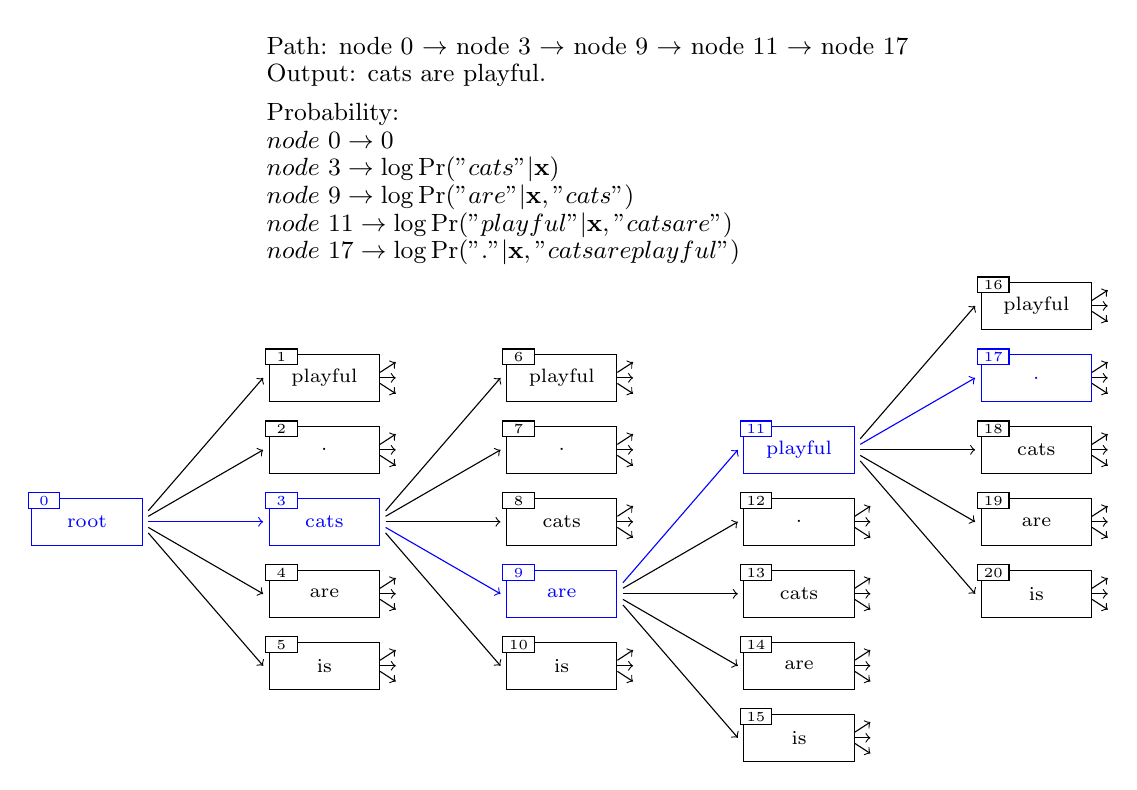
\begin{tikzpicture}
	
\def\ssep{1.6cm}

\tikzstyle{lnode} = [minimum width=1.4cm,minimum height=0.6cm,inner sep=0pt,draw,fill=white,rounded corners=0pt];
\tikzstyle{snode} = [minimum width=0.4cm,minimum height=0.2cm,inner sep=0pt,draw,fill=white];

\begin{scope}

% layer 0
\node [lnode,anchor=west,draw=blue] (node0) at (0,0) {\color{blue} \scriptsize{root}};

\node [snode,anchor=center,draw=blue] (label0) at ([xshift=0.16cm,yshift=-0.04cm]node0.north west) {\color{blue} \tiny{$0$}};

% layer 1
\node [lnode,anchor=west,draw=blue] (node13) at ([xshift=\ssep]node0.east) {\color{blue} \scriptsize{cats}};
\node [lnode,anchor=south west] (node12) at ([yshift=0.3cm]node13.north west) {\scriptsize{.}};
\node [lnode,anchor=south west] (node11) at ([yshift=0.3cm]node12.north west) {\scriptsize{playful}};
\node [lnode,anchor=north west] (node14) at ([yshift=-0.3cm]node13.south west) {\scriptsize{are}};
\node [lnode,anchor=north west] (node15) at ([yshift=-0.3cm]node14.south west) {\scriptsize{is}};

\node [snode,anchor=center] (label11) at ([xshift=0.16cm,yshift=-0.04cm]node11.north west) {\tiny{$1$}};
\node [snode,anchor=center] (label12) at ([xshift=0.16cm,yshift=-0.04cm]node12.north west) {\tiny{$2$}};
\node [snode,anchor=center,draw=blue] (label13) at ([xshift=0.16cm,yshift=-0.04cm]node13.north west) {\color{blue} \tiny{$3$}};
\node [snode,anchor=center] (label14) at ([xshift=0.16cm,yshift=-0.04cm]node14.north west) {\tiny{$4$}};
\node [snode,anchor=center] (label15) at ([xshift=0.16cm,yshift=-0.04cm]node15.north west) {\tiny{$5$}};

\draw [->] ([xshift=2pt,yshift=4pt]node0.east) -- ([xshift=-2pt]node11.west);
\draw [->] ([xshift=2pt,yshift=2pt]node0.east) -- ([xshift=-2pt]node12.west);
\draw [->,blue] ([xshift=2pt,yshift=0pt]node0.east) -- ([xshift=-2pt]node13.west);
\draw [->] ([xshift=2pt,yshift=-2pt]node0.east) -- ([xshift=-2pt]node14.west);
\draw [->] ([xshift=2pt,yshift=-4pt]node0.east) -- ([xshift=-2pt]node15.west);

% layer 2
\node [lnode,anchor=west] (node23) at ([xshift=\ssep]node13.east) {\scriptsize{cats}};
\node [lnode,anchor=south west] (node22) at ([yshift=0.3cm]node23.north west) {\scriptsize{.}};
\node [lnode,anchor=south west] (node21) at ([yshift=0.3cm]node22.north west) {\scriptsize{playful}};
\node [lnode,anchor=north west,draw=blue] (node24) at ([yshift=-0.3cm]node23.south west) {\color{blue} \scriptsize{are}};
\node [lnode,anchor=north west] (node25) at ([yshift=-0.3cm]node24.south west) {\scriptsize{is}};

\node [snode,anchor=center] (label21) at ([xshift=0.16cm,yshift=-0.04cm]node21.north west) {\tiny{$6$}};
\node [snode,anchor=center] (label22) at ([xshift=0.16cm,yshift=-0.04cm]node22.north west) {\tiny{$7$}};
\node [snode,anchor=center] (label23) at ([xshift=0.16cm,yshift=-0.04cm]node23.north west) {\tiny{$8$}};
\node [snode,anchor=center,draw=blue] (label24) at ([xshift=0.16cm,yshift=-0.04cm]node24.north west) {\color{blue} \tiny{$9$}};
\node [snode,anchor=center] (label25) at ([xshift=0.16cm,yshift=-0.04cm]node25.north west) {\tiny{$10$}};

\draw [->] ([xshift=2pt,yshift=4pt]node13.east) -- ([xshift=-2pt]node21.west);
\draw [->] ([xshift=2pt,yshift=2pt]node13.east) -- ([xshift=-2pt]node22.west);
\draw [->] ([xshift=2pt,yshift=0pt]node13.east) -- ([xshift=-2pt]node23.west);
\draw [->,blue] ([xshift=2pt,yshift=-2pt]node13.east) -- ([xshift=-2pt]node24.west);
\draw [->] ([xshift=2pt,yshift=-4pt]node13.east) -- ([xshift=-2pt]node25.west);

\draw [->] ([yshift=2pt]node11.east) -- ([yshift=0.2cm,xshift=0.2cm]node11.east);
\draw [->] ([yshift=0pt]node11.east) -- ([yshift=0.0cm,xshift=0.2cm]node11.east);
\draw [->] ([yshift=-2pt]node11.east) -- ([yshift=-0.2cm,xshift=0.2cm]node11.east);

\draw [->] ([yshift=2pt]node12.east) -- ([yshift=0.2cm,xshift=0.2cm]node12.east);
\draw [->] ([yshift=0pt]node12.east) -- ([yshift=0.0cm,xshift=0.2cm]node12.east);
\draw [->] ([yshift=-2pt]node12.east) -- ([yshift=-0.2cm,xshift=0.2cm]node12.east);

\draw [->] ([yshift=2pt]node14.east) -- ([yshift=0.2cm,xshift=0.2cm]node14.east);
\draw [->] ([yshift=0pt]node14.east) -- ([yshift=0.0cm,xshift=0.2cm]node14.east);
\draw [->] ([yshift=-2pt]node14.east) -- ([yshift=-0.2cm,xshift=0.2cm]node14.east);

\draw [->] ([yshift=2pt]node15.east) -- ([yshift=0.2cm,xshift=0.2cm]node15.east);
\draw [->] ([yshift=0pt]node15.east) -- ([yshift=0.0cm,xshift=0.2cm]node15.east);
\draw [->] ([yshift=-2pt]node15.east) -- ([yshift=-0.2cm,xshift=0.2cm]node15.east);

% layer 3
\node [lnode,anchor=west] (node33) at ([xshift=\ssep]node24.east) {\scriptsize{cats}};
\node [lnode,anchor=south west] (node32) at ([yshift=0.3cm]node33.north west) {\scriptsize{.}};
\node [lnode,anchor=south west,draw=blue] (node31) at ([yshift=0.3cm]node32.north west) {\color{blue} \scriptsize{playful}};
\node [lnode,anchor=north west] (node34) at ([yshift=-0.3cm]node33.south west) {\scriptsize{are}};
\node [lnode,anchor=north west] (node35) at ([yshift=-0.3cm]node34.south west) {\scriptsize{is}};

\node [snode,anchor=center,draw=blue] (label31) at ([xshift=0.16cm,yshift=-0.04cm]node31.north west) {\color{blue} \tiny{$11$}};
\node [snode,anchor=center] (label32) at ([xshift=0.16cm,yshift=-0.04cm]node32.north west) {\tiny{$12$}};
\node [snode,anchor=center] (label33) at ([xshift=0.16cm,yshift=-0.04cm]node33.north west) {\tiny{$13$}};
\node [snode,anchor=center] (label34) at ([xshift=0.16cm,yshift=-0.04cm]node34.north west) {\tiny{$14$}};
\node [snode,anchor=center] (label35) at ([xshift=0.16cm,yshift=-0.04cm]node35.north west) {\tiny{$15$}};

\draw [->,blue] ([xshift=2pt,yshift=4pt]node24.east) -- ([xshift=-2pt]node31.west);
\draw [->] ([xshift=2pt,yshift=2pt]node24.east) -- ([xshift=-2pt]node32.west);
\draw [->] ([xshift=2pt,yshift=0pt]node24.east) -- ([xshift=-2pt]node33.west);
\draw [->] ([xshift=2pt,yshift=-2pt]node24.east) -- ([xshift=-2pt]node34.west);
\draw [->] ([xshift=2pt,yshift=-4pt]node24.east) -- ([xshift=-2pt]node35.west);

\draw [->] ([yshift=2pt]node21.east) -- ([yshift=0.2cm,xshift=0.2cm]node21.east);
\draw [->] ([yshift=0pt]node21.east) -- ([yshift=0.0cm,xshift=0.2cm]node21.east);
\draw [->] ([yshift=-2pt]node21.east) -- ([yshift=-0.2cm,xshift=0.2cm]node21.east);

\draw [->] ([yshift=2pt]node22.east) -- ([yshift=0.2cm,xshift=0.2cm]node22.east);
\draw [->] ([yshift=0pt]node22.east) -- ([yshift=0.0cm,xshift=0.2cm]node22.east);
\draw [->] ([yshift=-2pt]node22.east) -- ([yshift=-0.2cm,xshift=0.2cm]node22.east);

\draw [->] ([yshift=2pt]node23.east) -- ([yshift=0.2cm,xshift=0.2cm]node23.east);
\draw [->] ([yshift=0pt]node23.east) -- ([yshift=0.0cm,xshift=0.2cm]node23.east);
\draw [->] ([yshift=-2pt]node23.east) -- ([yshift=-0.2cm,xshift=0.2cm]node23.east);

\draw [->] ([yshift=2pt]node25.east) -- ([yshift=0.2cm,xshift=0.2cm]node25.east);
\draw [->] ([yshift=0pt]node25.east) -- ([yshift=0.0cm,xshift=0.2cm]node25.east);
\draw [->] ([yshift=-2pt]node25.east) -- ([yshift=-0.2cm,xshift=0.2cm]node25.east);

% layer 4
\node [lnode,anchor=west] (node43) at ([xshift=\ssep]node31.east) {\scriptsize{cats}};
\node [lnode,anchor=south west,draw=blue] (node42) at ([yshift=0.3cm]node43.north west) {\color{blue} \scriptsize{.}};
\node [lnode,anchor=south west] (node41) at ([yshift=0.3cm]node42.north west) {\scriptsize{playful}};
\node [lnode,anchor=north west] (node44) at ([yshift=-0.3cm]node43.south west) {\scriptsize{are}};
\node [lnode,anchor=north west] (node45) at ([yshift=-0.3cm]node44.south west) {\scriptsize{is}};

\node [snode,anchor=center] (label41) at ([xshift=0.16cm,yshift=-0.04cm]node41.north west) {\tiny{$16$}};
\node [snode,anchor=center,draw=blue] (label42) at ([xshift=0.16cm,yshift=-0.04cm]node42.north west) {\color{blue} \tiny{$17$}};
\node [snode,anchor=center] (label43) at ([xshift=0.16cm,yshift=-0.04cm]node43.north west) {\tiny{$18$}};
\node [snode,anchor=center] (label44) at ([xshift=0.16cm,yshift=-0.04cm]node44.north west) {\tiny{$19$}};
\node [snode,anchor=center] (label45) at ([xshift=0.16cm,yshift=-0.04cm]node45.north west) {\tiny{$20$}};

\draw [->] ([xshift=2pt,yshift=4pt]node31.east) -- ([xshift=-2pt]node41.west);
\draw [->,blue] ([xshift=2pt,yshift=2pt]node31.east) -- ([xshift=-2pt]node42.west);
\draw [->] ([xshift=2pt,yshift=0pt]node31.east) -- ([xshift=-2pt]node43.west);
\draw [->] ([xshift=2pt,yshift=-2pt]node31.east) -- ([xshift=-2pt]node44.west);
\draw [->] ([xshift=2pt,yshift=-4pt]node31.east) -- ([xshift=-2pt]node45.west);

\draw [->] ([yshift=2pt]node32.east) -- ([yshift=0.2cm,xshift=0.2cm]node32.east);
\draw [->] ([yshift=0pt]node32.east) -- ([yshift=0.0cm,xshift=0.2cm]node32.east);
\draw [->] ([yshift=-2pt]node32.east) -- ([yshift=-0.2cm,xshift=0.2cm]node32.east);

\draw [->] ([yshift=2pt]node33.east) -- ([yshift=0.2cm,xshift=0.2cm]node33.east);
\draw [->] ([yshift=0pt]node33.east) -- ([yshift=0.0cm,xshift=0.2cm]node33.east);
\draw [->] ([yshift=-2pt]node33.east) -- ([yshift=-0.2cm,xshift=0.2cm]node33.east);

\draw [->] ([yshift=2pt]node34.east) -- ([yshift=0.2cm,xshift=0.2cm]node34.east);
\draw [->] ([yshift=0pt]node34.east) -- ([yshift=0.0cm,xshift=0.2cm]node34.east);
\draw [->] ([yshift=-2pt]node34.east) -- ([yshift=-0.2cm,xshift=0.2cm]node34.east);

\draw [->] ([yshift=2pt]node35.east) -- ([yshift=0.2cm,xshift=0.2cm]node35.east);
\draw [->] ([yshift=0pt]node35.east) -- ([yshift=0.0cm,xshift=0.2cm]node35.east);
\draw [->] ([yshift=-2pt]node35.east) -- ([yshift=-0.2cm,xshift=0.2cm]node35.east);

\draw [->] ([yshift=2pt]node41.east) -- ([yshift=0.2cm,xshift=0.2cm]node41.east);
\draw [->] ([yshift=0pt]node41.east) -- ([yshift=0.0cm,xshift=0.2cm]node41.east);
\draw [->] ([yshift=-2pt]node41.east) -- ([yshift=-0.2cm,xshift=0.2cm]node41.east);

\draw [->] ([yshift=2pt]node42.east) -- ([yshift=0.2cm,xshift=0.2cm]node42.east);
\draw [->] ([yshift=0pt]node42.east) -- ([yshift=0.0cm,xshift=0.2cm]node42.east);
\draw [->] ([yshift=-2pt]node42.east) -- ([yshift=-0.2cm,xshift=0.2cm]node42.east);

\draw [->] ([yshift=2pt]node43.east) -- ([yshift=0.2cm,xshift=0.2cm]node43.east);
\draw [->] ([yshift=0pt]node43.east) -- ([yshift=0.0cm,xshift=0.2cm]node43.east);
\draw [->] ([yshift=-2pt]node43.east) -- ([yshift=-0.2cm,xshift=0.2cm]node43.east);

\draw [->] ([yshift=2pt]node44.east) -- ([yshift=0.2cm,xshift=0.2cm]node44.east);
\draw [->] ([yshift=0pt]node44.east) -- ([yshift=0.0cm,xshift=0.2cm]node44.east);
\draw [->] ([yshift=-2pt]node44.east) -- ([yshift=-0.2cm,xshift=0.2cm]node44.east);

\draw [->] ([yshift=2pt]node45.east) -- ([yshift=0.2cm,xshift=0.2cm]node45.east);
\draw [->] ([yshift=0pt]node45.east) -- ([yshift=0.0cm,xshift=0.2cm]node45.east);
\draw [->] ([yshift=-2pt]node45.east) -- ([yshift=-0.2cm,xshift=0.2cm]node45.east);

\node [anchor=south west,align=left] (pathdescription) at ([yshift=1cm,xshift=-0.15cm]node11.north west) {\small{Path: node $0$ $\to$ node $3$ $\to$ node $9$ $\to$ node $11$ $\to$ node $17$}\\[-2pt] \small{Output: cats are playful.}\\[2pt] \small{Probability:}\\[-2pt] \small{$\text{node}\ 0 \to 0$} \\[-2pt] \small{$\text{node}\ 3 \to \log \Pr(\text{"cats"}|\mathbf{x})$}\\[-2pt] \small{$\text{node}\ 9 \to \log \Pr(\text{"are"}|\mathbf{x},\text{"cats"})$}\\[-2pt] \small{$\text{node}\ 11 \to \log \Pr(\text{"playful"}|\mathbf{x},\text{"cats are"})$}\\[-2pt] \small{$\text{node}\ 17 \to \log \Pr(\text{"."}|\mathbf{x},\text{"cats are playful"})$}};

\end{scope}

\end{tikzpicture}
\end{center}

\vspace{-0.5cm} \caption{A search tree for decoding. At each node, we expand the tree by considering all possible tokens, each leading to a new node representing a potential continuation of the text. Here we highlight a path through nodes 0, 3, 9, 11, and 17. The path represents the output sequence ``\textit{cats are playful.}'', whose log-probability can be computed by accumulating the log-probabilities of these nodes.}
\label{fig:llm-decoding-search-tree}
\end{figure}

In general, the search tree is organized into levels, where each level consists of all nodes at the same depth. Thus, the tree can be viewed as being expanded level by level, where each level corresponds to one decoding step. As the search progresses, new tokens are appended to these sequences, expanding them incrementally.

Let $Y_i$ be the set of the sequences that the LLM generates at step $i$. $Y_i$ can be obtained by expanding each sequence in $Y_{i-1}$ with all possible next tokens in the vocabulary $V$, given in the following recursive form:
\begin{eqnarray}
Y_i & = & Y_{i-1} \times V,
\end{eqnarray}

\noindent where $Y_{i-1} \times V$ denotes the Cartesian product of $Y_{i-1}$ and $V$ (i.e., each sequence in $Y_{i-1}$ is concatenated with each token in $V$). Note that if a sequence in $Y_{i-1}$ is complete (e.g., ending with the $\langle \mathrm{EOS} \rangle$ token), it will not be expanded any further. Let $\Psi(Y_i)$ be the set of all complete sequences in $Y_i$. Then, the search space can be expressed as:
\begin{eqnarray}
\mathcal{Y} & = & \Psi(Y_1) \bigcup \Psi(Y_2) \bigcup \cdots \bigcup \Psi(Y_{n_{\mathrm{max}}}),
\end{eqnarray}

\noindent where $n_{\mathrm{max}}$ is the maximum length of a sequence.

Most decoding algorithms follow this level-by-level search process. However, $\mathcal{Y}$ consists of an exponentially large number of sequences, and a direct search
in such a vast space is computationally infeasible. Therefore, practical decoding algorithms often rely on strategies to prune the search space and avoid exploring low-quality sequences. For example, at each decoding step, $Y_i$ can be obtained in the following way:
\begin{eqnarray}
Y_i & = & \mathrm{Prune}(Y_{i-1} \times V),
\end{eqnarray}

\noindent where $\mathrm{Prune}(\cdot)$ is a function that selectively removes sequences less likely to result in high-quality outcomes. In general, we expect that $|Y_i| \ll |Y_{i-1}| \cdot |V|$. Thus we can drastically reduce the number of sequences under consideration at each step, ensuring that the computational load does not grow exponentially with the sequence length.

Next, we will introduce these decoding algorithms. Some of them have already been discussed in sequence-to-sequence models, while others are more commonly used in LLMs.

\subsubsection{Greedy Decoding}

Greedy search (or greedy decoding) is one of the most widely used decoding methods in NLP, particularly in text generation tasks like machine translation. The idea behind greedy search is straightforward: at each step in generation, it selects the next token that has the highest prediction probability. For each sequence $\mathbf{y} = y_1\cdots y_i \in Y_{i-1} \times V$, we can evaluate it using
$\log \Pr(\mathbf{y}|\mathbf{x})$. This log-probability can be easily computed by noting that:
\begin{eqnarray}
\log \Pr(\mathbf{y}|\mathbf{x}) & = & \log \Pr(y_1\cdots y_i|\mathbf{x}) \nonumber \\
& = & \underbrace{\log \Pr(\mathbf{y}_{<i}|\mathbf{x})}_{\text{accumulated up to the parent node}} + \underbrace{\log \Pr(y_i|\mathbf{x},\mathbf{y}_{<i})}_{\text{newly computed for the current node}},
\end{eqnarray}

\noindent Here the first term is the sum of the log-probabilities of the path from the root to the parent node, which has been computed in the previous decoding steps. At step $i$, we only need to compute the second term which is the standard token prediction log-probability produced by the LLM.

The ``best'' token at step $i$ is then chosen as:
\begin{eqnarray}
y_i^{\mathrm{top}1} & = & \argmax_{y_i \in V} \log \Pr(y_1\cdots y_i|\mathbf{x}) \nonumber \\
                    & = & \argmax_{y_i \in V} \big[ \underbrace{\log \Pr(\mathbf{y}_{<i}|\mathbf{x})}_{\text{fixed wrt. $y_i$}} + \log \Pr(y_i|\mathbf{x},\mathbf{y}_{<i}) \big] \nonumber \\
                    & = & \argmax_{y_i \in V} \log \Pr(y_i|\mathbf{x},\mathbf{y}_{<i}).
\end{eqnarray}

Thus, the ``best'' sequence generated up to step $i$ is given by:
\begin{eqnarray}
\mathbf{y}^{\mathrm{top}1} & = & y_1\cdots y_{i-1} y_i^{\mathrm{top}1}.
\end{eqnarray}

Finally, $Y_i$ contains only this sequence:
\begin{eqnarray}
Y_i & = & \{\mathbf{y}^{\mathrm{top}1}\}.
\end{eqnarray}

The greedy choice in one decoding step is illustrated in Figure~\ref{fig:llm-decoding-methods} (a). Greedy search offers computational efficiency and is simple to implement. Its primary disadvantage, however, lies in its suboptimal nature --- high-quality sequences are likely pruned at early stages of decoding. Therefore, greedy search is appealing for tasks that demand speed and simplicity. For tasks that require better search results, alternative strategies such as beam search, which explores multiple potential paths simultaneously, are preferable.

\begin{figure}[!t]
\centering
% !Mode:: "TeX:UTF-8"
% !TEX encoding = UTF-8 Unicode

\begin{center}
\begin{tikzpicture}
	
\def\ssep{1.2cm}

\tikzstyle{lnode} = [minimum width=1.0cm,minimum height=0.4cm,inner sep=0pt,draw,fill=white,rounded corners=0pt];
\tikzstyle{snode} = [minimum width=0.27cm,minimum height=0.18cm,inner sep=0pt,draw,fill=white];

% greedy search
\begin{scope}

\node [lnode,anchor=west] (node0) at (0,0) {\scriptsize{is}};

\node [snode,anchor=center] (label0) at ([xshift=0.10cm,yshift=-0.03cm]node0.north west) {\tiny{$4$}};

\node [lnode,anchor=west] (node13) at ([xshift=\ssep]node0.east) {\scriptsize{on}};
\node [lnode,anchor=south west] (node12) at ([yshift=0.3cm]node13.north west) {\scriptsize{cute}};
\node [lnode,anchor=south west] (node11) at ([yshift=0.3cm]node12.north west) {\scriptsize{.}};
\node [lnode,anchor=north west] (node14) at ([yshift=-0.3cm]node13.south west) {\scriptsize{are}};
\node [lnode,anchor=north west] (node15) at ([yshift=-0.3cm]node14.south west) {\scriptsize{sick}};

\node [snode,anchor=center,fill=red!30] (label11) at ([xshift=0.10cm,yshift=-0.03cm]node11.north west) {\tiny{$5$}};
\node [snode,anchor=center,fill=ugreen!30] (label12) at ([xshift=0.10cm,yshift=-0.03cm]node12.north west) {\tiny{$6$}};
\node [snode,anchor=center,fill=blue!30] (label13) at ([xshift=0.10cm,yshift=-0.03cm]node13.north west) {\tiny{$7$}};
\node [snode,anchor=center,fill=orange!30] (label14) at ([xshift=0.10cm,yshift=-0.03cm]node14.north west) {\tiny{$8$}};
\node [snode,anchor=center,fill=purple!30] (label15) at ([xshift=0.10cm,yshift=-0.03cm]node15.north west) {\tiny{$9$}};

\draw [->] ([xshift=2pt,yshift=4pt]node0.east) -- ([xshift=-2pt]node11.west);
\draw [->] ([xshift=2pt,yshift=2pt]node0.east) -- ([xshift=-2pt]node12.west);
\draw [->] ([xshift=2pt,yshift=0pt]node0.east) -- ([xshift=-2pt]node13.west);
\draw [->] ([xshift=2pt,yshift=-2pt]node0.east) -- ([xshift=-2pt]node14.west);
\draw [->] ([xshift=2pt,yshift=-4pt]node0.east) -- ([xshift=-2pt]node15.west);

\node [anchor=north] (step1label) at ([yshift=0.7cm,xshift=-0.5cm]node11.north west) {\footnotesize{\ding{172} Expansion}};

\node [lnode,anchor=west] (node21) at ([xshift=1.3*\ssep]node11.east) {\scriptsize{cute}};
\node [lnode,anchor=west] (node22) at ([xshift=1.3*\ssep]node12.east) {\scriptsize{on}};
\node [lnode,anchor=west] (node23) at ([xshift=1.3*\ssep]node13.east) {\scriptsize{sick}};
\node [lnode,anchor=west] (node24) at ([xshift=1.3*\ssep]node14.east) {\scriptsize{are}};
\node [lnode,anchor=west] (node25) at ([xshift=1.3*\ssep]node15.east) {\scriptsize{.}};

\node [snode,anchor=center,fill=ugreen!30] (label21) at ([xshift=0.10cm,yshift=-0.03cm]node21.north west) {\tiny{$6$}};
\node [snode,anchor=center,fill=blue!30] (label22) at ([xshift=0.10cm,yshift=-0.03cm]node22.north west) {\tiny{$7$}};
\node [snode,anchor=center,fill=purple!30] (label23) at ([xshift=0.10cm,yshift=-0.03cm]node23.north west) {\tiny{$9$}};
\node [snode,anchor=center,fill=orange!30] (label24) at ([xshift=0.10cm,yshift=-0.03cm]node24.north west) {\tiny{$8$}};
\node [snode,anchor=center,fill=red!30] (label25) at ([xshift=0.10cm,yshift=-0.03cm]node25.north west) {\tiny{$5$}};

\node [anchor=west] (p21) at (node21.east) {\tiny{$\Pr=.34$}};
\node [anchor=west] (p22) at (node22.east) {\tiny{$\Pr=.32$}};
\node [anchor=west] (p23) at (node23.east) {\tiny{$\Pr=.21$}};
\node [anchor=west] (p24) at (node24.east) {\tiny{$\Pr=.12$}};
\node [anchor=west] (p25) at (node25.east) {\tiny{$\Pr=.01$}};

\node [anchor=west,fill=gray!30,inner sep=3pt] (p21label) at ([xshift=-0.05cm]p21.east) {\tiny{\underline{ok}}};
\node [anchor=west,inner sep=3pt] (p22label) at ([xshift=-0.05cm]p22.east) {\tiny{\underline{pruned}}};
\node [anchor=west,inner sep=3pt] (p23label) at ([xshift=-0.05cm]p23.east) {\tiny{\underline{pruned}}};
\node [anchor=west,inner sep=3pt] (p24label) at ([xshift=-0.05cm]p24.east) {\tiny{\underline{pruned}}};
\node [anchor=west,inner sep=3pt] (p25label) at ([xshift=-0.05cm]p25.east) {\tiny{\underline{pruned}}};

\node [anchor=north west] (step2label) at ([yshift=0.7cm,xshift=-0.2cm]node21.north west) {\footnotesize{\ding{173} Ranking}};

\node [lnode,anchor=west] (node31) at ([xshift=2*\ssep]node21.east) {\scriptsize{cute}};
%\node [lnode,anchor=west] (node32) at ([xshift=2*\ssep]node22.east) {\scriptsize{on}};
%\node [lnode,anchor=west] (node33) at ([xshift=2*\ssep]node23.east) {\scriptsize{sick}};
%\node [lnode,anchor=west] (node34) at ([xshift=2*\ssep]node24.east) {\scriptsize{are}};
%\node [lnode,anchor=west] (node35) at ([xshift=2*\ssep]node25.east) {\scriptsize{.}};

\node [snode,anchor=center,fill=ugreen!30] (label31) at ([xshift=0.10cm,yshift=-0.03cm]node31.north west) {\tiny{$6$}};
%\node [snode,anchor=center,fill=blue!30] (label32) at ([xshift=0.10cm,yshift=-0.03cm]node32.north west) {\tiny{$7$}};
%\node [snode,anchor=center,fill=purple!30] (label33) at ([xshift=0.10cm,yshift=-0.03cm]node33.north west) {\tiny{$9$}};
%\node [snode,anchor=center,fill=orange!30] (label34) at ([xshift=0.10cm,yshift=-0.03cm]node34.north west) {\tiny{$8$}};
%\node [snode,anchor=center,fill=red!30] (label35) at ([xshift=0.10cm,yshift=-0.03cm]node35.north west) {\tiny{$5$}};

\node [anchor=east] (selectionarrow) at (node31.west) {\small{$\Longrightarrow$}};

%\node [anchor=west] (p31) at (node31.east) {\tiny{$\Pr=.34$}};
%\node [anchor=west] (p32) at (node32.east) {\tiny{$\Pr=.32$}};
%\node [anchor=west] (p33) at (node33.east) {\tiny{$\Pr=.21$}};
%\node [anchor=west] (p34) at (node34.east) {\tiny{$\Pr=.12$}};
%\node [anchor=west] (p35) at (node35.east) {\tiny{$\Pr=.01$}};

\node [anchor=north west,align=left] (step3label) at ([yshift=0.7cm,xshift=-0.2cm]node31.north west) {\footnotesize{\ding{174} Output (1-best)}};

%\node [lnode,anchor=west] (node41) at ([xshift=2*\ssep]node31.east) {\scriptsize{cute}};
%\node [lnode,anchor=west] (node42) at ([xshift=2*\ssep]node32.east) {\scriptsize{on}};
%\node [lnode,anchor=west] (node43) at ([xshift=2*\ssep]node33.east) {\scriptsize{sick}};
%\node [lnode,anchor=west] (node44) at ([xshift=2*\ssep]node34.east) {\scriptsize{are}};
%\node [lnode,anchor=west] (node45) at ([xshift=2*\ssep]node35.east) {\scriptsize{.}};

%\node [snode,anchor=center,fill=ugreen!30] (label41) at ([xshift=0.10cm,yshift=-0.03cm]node41.north west) {\tiny{$6$}};
%\node [snode,anchor=center,fill=blue!30] (label42) at ([xshift=0.10cm,yshift=-0.03cm]node42.north west) {\tiny{$7$}};
%\node [snode,anchor=center,fill=purple!30] (label43) at ([xshift=0.10cm,yshift=-0.03cm]node43.north west) {\tiny{$9$}};
%\node [snode,anchor=center,fill=orange!30] (label44) at ([xshift=0.10cm,yshift=-0.03cm]node44.north west) {\tiny{$8$}};
%\node [snode,anchor=center,fill=red!30] (label45) at ([xshift=0.10cm,yshift=-0.03cm]node45.north west) {\tiny{$5$}};

%\node [anchor=north west] (step4label) at ([yshift=0.9cm,xshift=-0.2cm]node41.north west) {\footnotesize{\ding{175} Output}};

\node [anchor=north] (caption) at ([yshift=-0.2cm,xshift=1cm]node25.south east) {\small{(a) Greedy search}};

\end{scope}

% beam search
\begin{scope}[yshift=-5.0cm]

\node [lnode,anchor=west] (node0) at (0,0) {\scriptsize{is}};

\node [snode,anchor=center] (label0) at ([xshift=0.10cm,yshift=-0.03cm]node0.north west) {\tiny{$4$}};

\node [lnode,anchor=west] (node13) at ([xshift=\ssep]node0.east) {\scriptsize{on}};
\node [lnode,anchor=south west] (node12) at ([yshift=0.3cm]node13.north west) {\scriptsize{cute}};
\node [lnode,anchor=south west] (node11) at ([yshift=0.3cm]node12.north west) {\scriptsize{.}};
\node [lnode,anchor=north west] (node14) at ([yshift=-0.3cm]node13.south west) {\scriptsize{are}};
\node [lnode,anchor=north west] (node15) at ([yshift=-0.3cm]node14.south west) {\scriptsize{sick}};

\node [snode,anchor=center,fill=red!30] (label11) at ([xshift=0.10cm,yshift=-0.03cm]node11.north west) {\tiny{$5$}};
\node [snode,anchor=center,fill=ugreen!30] (label12) at ([xshift=0.10cm,yshift=-0.03cm]node12.north west) {\tiny{$6$}};
\node [snode,anchor=center,fill=blue!30] (label13) at ([xshift=0.10cm,yshift=-0.03cm]node13.north west) {\tiny{$7$}};
\node [snode,anchor=center,fill=orange!30] (label14) at ([xshift=0.10cm,yshift=-0.03cm]node14.north west) {\tiny{$8$}};
\node [snode,anchor=center,fill=purple!30] (label15) at ([xshift=0.10cm,yshift=-0.03cm]node15.north west) {\tiny{$9$}};

\draw [->] ([xshift=2pt,yshift=4pt]node0.east) -- ([xshift=-2pt]node11.west);
\draw [->] ([xshift=2pt,yshift=2pt]node0.east) -- ([xshift=-2pt]node12.west);
\draw [->] ([xshift=2pt,yshift=0pt]node0.east) -- ([xshift=-2pt]node13.west);
\draw [->] ([xshift=2pt,yshift=-2pt]node0.east) -- ([xshift=-2pt]node14.west);
\draw [->] ([xshift=2pt,yshift=-4pt]node0.east) -- ([xshift=-2pt]node15.west);

\node [anchor=north] (step1label) at ([yshift=0.7cm,xshift=-0.5cm]node11.north west) {\footnotesize{\ding{172} Expansion}};

\node [lnode,anchor=west] (node21) at ([xshift=1.3*\ssep]node11.east) {\scriptsize{cute}};
\node [lnode,anchor=west] (node22) at ([xshift=1.3*\ssep]node12.east) {\scriptsize{on}};
\node [lnode,anchor=west] (node23) at ([xshift=1.3*\ssep]node13.east) {\scriptsize{sick}};
\node [lnode,anchor=west] (node24) at ([xshift=1.3*\ssep]node14.east) {\scriptsize{are}};
\node [lnode,anchor=west] (node25) at ([xshift=1.3*\ssep]node15.east) {\scriptsize{.}};

\node [snode,anchor=center,fill=ugreen!30] (label21) at ([xshift=0.10cm,yshift=-0.03cm]node21.north west) {\tiny{$6$}};
\node [snode,anchor=center,fill=blue!30] (label22) at ([xshift=0.10cm,yshift=-0.03cm]node22.north west) {\tiny{$7$}};
\node [snode,anchor=center,fill=purple!30] (label23) at ([xshift=0.10cm,yshift=-0.03cm]node23.north west) {\tiny{$9$}};
\node [snode,anchor=center,fill=orange!30] (label24) at ([xshift=0.10cm,yshift=-0.03cm]node24.north west) {\tiny{$8$}};
\node [snode,anchor=center,fill=red!30] (label25) at ([xshift=0.10cm,yshift=-0.03cm]node25.north west) {\tiny{$5$}};

\node [anchor=west] (p21) at (node21.east) {\tiny{$\Pr=.34$}};
\node [anchor=west] (p22) at (node22.east) {\tiny{$\Pr=.32$}};
\node [anchor=west] (p23) at (node23.east) {\tiny{$\Pr=.21$}};
\node [anchor=west] (p24) at (node24.east) {\tiny{$\Pr=.12$}};
\node [anchor=west] (p25) at (node25.east) {\tiny{$\Pr=.01$}};

\node [anchor=west,fill=gray!30,inner sep=3pt] (p21label) at ([xshift=-0.05cm]p21.east) {\tiny{\underline{ok}}};
\node [anchor=west,fill=gray!30,inner sep=3pt] (p22label) at ([xshift=-0.05cm]p22.east) {\tiny{\underline{ok}}};
\node [anchor=west,fill=gray!30,inner sep=3pt] (p23label) at ([xshift=-0.05cm]p23.east) {\tiny{\underline{ok}}};
\node [anchor=west,inner sep=3pt] (p24label) at ([xshift=-0.05cm]p24.east) {\tiny{\underline{pruned}}};
\node [anchor=west,inner sep=3pt] (p25label) at ([xshift=-0.05cm]p25.east) {\tiny{\underline{pruned}}};

\node [anchor=north west] (step2label) at ([yshift=0.7cm,xshift=-0.2cm]node21.north west) {\footnotesize{\ding{173} Ranking}};

\node [lnode,anchor=west] (node31) at ([xshift=2*\ssep]node21.east) {\scriptsize{cute}};
\node [lnode,anchor=west] (node32) at ([xshift=2*\ssep]node22.east) {\scriptsize{on}};
\node [lnode,anchor=west] (node33) at ([xshift=2*\ssep]node23.east) {\scriptsize{sick}};
%\node [lnode,anchor=west] (node34) at ([xshift=2*\ssep]node24.east) {\scriptsize{are}};
%\node [lnode,anchor=west] (node35) at ([xshift=2*\ssep]node25.east) {\scriptsize{.}};

\node [snode,anchor=center,fill=ugreen!30] (label31) at ([xshift=0.10cm,yshift=-0.03cm]node31.north west) {\tiny{$6$}};
\node [snode,anchor=center,fill=blue!30] (label32) at ([xshift=0.10cm,yshift=-0.03cm]node32.north west) {\tiny{$7$}};
\node [snode,anchor=center,fill=purple!30] (label33) at ([xshift=0.10cm,yshift=-0.03cm]node33.north west) {\tiny{$9$}};
%\node [snode,anchor=center,fill=orange!30] (label34) at ([xshift=0.10cm,yshift=-0.03cm]node34.north west) {\tiny{$8$}};
%\node [snode,anchor=center,fill=red!30] (label35) at ([xshift=0.10cm,yshift=-0.03cm]node35.north west) {\tiny{$5$}};

\node [anchor=east] (selectionarrow) at (node31.west) {\small{$\Longrightarrow$}};
\node [anchor=east] (selectionarrow) at (node32.west) {\small{$\Longrightarrow$}};
\node [anchor=east] (selectionarrow) at (node33.west) {\small{$\Longrightarrow$}};

%\node [anchor=west] (p31) at (node31.east) {\tiny{$\Pr=.34$}};
%\node [anchor=west] (p32) at (node32.east) {\tiny{$\Pr=.32$}};
%\node [anchor=west] (p33) at (node33.east) {\tiny{$\Pr=.21$}};
%\node [anchor=west] (p34) at (node34.east) {\tiny{$\Pr=.12$}};
%\node [anchor=west] (p35) at (node35.east) {\tiny{$\Pr=.01$}};

\node [anchor=north west,align=left] (step3label) at ([yshift=0.7cm,xshift=-0.2cm]node31.north west) {\footnotesize{\ding{174} Output ($K$-best)}};

%\node [lnode,anchor=west] (node41) at ([xshift=2*\ssep]node31.east) {\scriptsize{cute}};
%\node [lnode,anchor=west] (node42) at ([xshift=2*\ssep]node32.east) {\scriptsize{on}};
%\node [lnode,anchor=west] (node43) at ([xshift=2*\ssep]node33.east) {\scriptsize{sick}};
%\node [lnode,anchor=west] (node44) at ([xshift=2*\ssep]node34.east) {\scriptsize{are}};
%\node [lnode,anchor=west] (node45) at ([xshift=2*\ssep]node35.east) {\scriptsize{.}};

%\node [snode,anchor=center,fill=ugreen!30] (label41) at ([xshift=0.10cm,yshift=-0.03cm]node41.north west) {\tiny{$6$}};
%\node [snode,anchor=center,fill=blue!30] (label42) at ([xshift=0.10cm,yshift=-0.03cm]node42.north west) {\tiny{$7$}};
%\node [snode,anchor=center,fill=purple!30] (label43) at ([xshift=0.10cm,yshift=-0.03cm]node43.north west) {\tiny{$9$}};
%\node [snode,anchor=center,fill=orange!30] (label44) at ([xshift=0.10cm,yshift=-0.03cm]node44.north west) {\tiny{$8$}};
%\node [snode,anchor=center,fill=red!30] (label45) at ([xshift=0.10cm,yshift=-0.03cm]node45.north west) {\tiny{$5$}};

%\node [anchor=north west] (step4label) at ([yshift=0.9cm,xshift=-0.2cm]node41.north west) {\footnotesize{\ding{175} Output}};

\draw [decoration={brace,amplitude=4pt},decorate] ([xshift=0.2cm]node31.north east) -- ([xshift=0.2cm]node33.south east) node [pos=0.5,right,xshift=0.1cm] {\footnotesize{beam width ($K$) = $3$}};

\node [anchor=north] (caption) at ([yshift=-0.2cm,xshift=1cm]node25.south east) {\small{(b) Beam search}};

\end{scope}

% top-k sampling
\begin{scope}[yshift=-10.0cm]

\node [lnode,anchor=west] (node0) at (0,0) {\scriptsize{is}};

\node [snode,anchor=center] (label0) at ([xshift=0.10cm,yshift=-0.03cm]node0.north west) {\tiny{$4$}};

\node [lnode,anchor=west] (node13) at ([xshift=\ssep]node0.east) {\scriptsize{on}};
\node [lnode,anchor=south west] (node12) at ([yshift=0.3cm]node13.north west) {\scriptsize{cute}};
\node [lnode,anchor=south west] (node11) at ([yshift=0.3cm]node12.north west) {\scriptsize{.}};
\node [lnode,anchor=north west] (node14) at ([yshift=-0.3cm]node13.south west) {\scriptsize{are}};
\node [lnode,anchor=north west] (node15) at ([yshift=-0.3cm]node14.south west) {\scriptsize{sick}};

\node [snode,anchor=center,fill=red!30] (label11) at ([xshift=0.10cm,yshift=-0.03cm]node11.north west) {\tiny{$5$}};
\node [snode,anchor=center,fill=ugreen!30] (label12) at ([xshift=0.10cm,yshift=-0.03cm]node12.north west) {\tiny{$6$}};
\node [snode,anchor=center,fill=blue!30] (label13) at ([xshift=0.10cm,yshift=-0.03cm]node13.north west) {\tiny{$7$}};
\node [snode,anchor=center,fill=orange!30] (label14) at ([xshift=0.10cm,yshift=-0.03cm]node14.north west) {\tiny{$8$}};
\node [snode,anchor=center,fill=purple!30] (label15) at ([xshift=0.10cm,yshift=-0.03cm]node15.north west) {\tiny{$9$}};

\draw [->] ([xshift=2pt,yshift=4pt]node0.east) -- ([xshift=-2pt]node11.west);
\draw [->] ([xshift=2pt,yshift=2pt]node0.east) -- ([xshift=-2pt]node12.west);
\draw [->] ([xshift=2pt,yshift=0pt]node0.east) -- ([xshift=-2pt]node13.west);
\draw [->] ([xshift=2pt,yshift=-2pt]node0.east) -- ([xshift=-2pt]node14.west);
\draw [->] ([xshift=2pt,yshift=-4pt]node0.east) -- ([xshift=-2pt]node15.west);

\node [anchor=north] (step1label) at ([yshift=0.7cm,xshift=-0.5cm]node11.north west) {\footnotesize{\ding{172} Expansion}};

\node [lnode,anchor=west] (node21) at ([xshift=1.3*\ssep]node11.east) {\scriptsize{cute}};
\node [lnode,anchor=west] (node22) at ([xshift=1.3*\ssep]node12.east) {\scriptsize{on}};
\node [lnode,anchor=west] (node23) at ([xshift=1.3*\ssep]node13.east) {\scriptsize{sick}};
\node [lnode,anchor=west] (node24) at ([xshift=1.3*\ssep]node14.east) {\scriptsize{are}};
\node [lnode,anchor=west] (node25) at ([xshift=1.3*\ssep]node15.east) {\scriptsize{.}};

\node [snode,anchor=center,fill=ugreen!30] (label21) at ([xshift=0.10cm,yshift=-0.03cm]node21.north west) {\tiny{$6$}};
\node [snode,anchor=center,fill=blue!30] (label22) at ([xshift=0.10cm,yshift=-0.03cm]node22.north west) {\tiny{$7$}};
\node [snode,anchor=center,fill=purple!30] (label23) at ([xshift=0.10cm,yshift=-0.03cm]node23.north west) {\tiny{$9$}};
\node [snode,anchor=center,fill=orange!30] (label24) at ([xshift=0.10cm,yshift=-0.03cm]node24.north west) {\tiny{$8$}};
\node [snode,anchor=center,fill=red!30] (label25) at ([xshift=0.10cm,yshift=-0.03cm]node25.north west) {\tiny{$5$}};

\node [anchor=west] (p21) at (node21.east) {\tiny{$\Pr=.34$}};
\node [anchor=west] (p22) at (node22.east) {\tiny{$\Pr=.32$}};
\node [anchor=west] (p23) at (node23.east) {\tiny{$\Pr=.21$}};
\node [anchor=west] (p24) at (node24.east) {\tiny{$\Pr=.12$}};
\node [anchor=west] (p25) at (node25.east) {\tiny{$\Pr=.01$}};

\node [anchor=west,fill=gray!30,inner sep=3pt] (p21label) at ([xshift=-0.05cm]p21.east) {\tiny{\underline{ok}}};
\node [anchor=west,fill=gray!30,inner sep=3pt] (p22label) at ([xshift=-0.05cm]p22.east) {\tiny{\underline{ok}}};
\node [anchor=west,fill=gray!30,inner sep=3pt] (p23label) at ([xshift=-0.05cm]p23.east) {\tiny{\underline{ok}}};
\node [anchor=west,inner sep=3pt] (p24label) at ([xshift=-0.05cm]p24.east) {\tiny{\underline{pruned}}};
\node [anchor=west,inner sep=3pt] (p25label) at ([xshift=-0.05cm]p25.east) {\tiny{\underline{pruned}}};

\node [anchor=north west] (step2label) at ([yshift=0.7cm,xshift=-0.2cm]node21.north west) {\footnotesize{\ding{173} Ranking}};

\node [lnode,anchor=west] (node31) at ([xshift=2*\ssep]node21.east) {\scriptsize{cute}};
\node [lnode,anchor=west] (node32) at ([xshift=2*\ssep]node22.east) {\scriptsize{on}};
\node [lnode,anchor=west] (node33) at ([xshift=2*\ssep]node23.east) {\scriptsize{sick}};
%\node [lnode,anchor=west] (node34) at ([xshift=2*\ssep]node24.east) {\scriptsize{are}};
%\node [lnode,anchor=west] (node35) at ([xshift=2*\ssep]node25.east) {\scriptsize{.}};

\node [snode,anchor=center,fill=ugreen!30] (label31) at ([xshift=0.10cm,yshift=-0.03cm]node31.north west) {\tiny{$6$}};
\node [snode,anchor=center,fill=blue!30] (label32) at ([xshift=0.10cm,yshift=-0.03cm]node32.north west) {\tiny{$7$}};
\node [snode,anchor=center,fill=purple!30] (label33) at ([xshift=0.10cm,yshift=-0.03cm]node33.north west) {\tiny{$9$}};
%\node [snode,anchor=center,fill=orange!30] (label34) at ([xshift=0.10cm,yshift=-0.03cm]node34.north west) {\tiny{$8$}};
%\node [snode,anchor=center,fill=red!30] (label35) at ([xshift=0.10cm,yshift=-0.03cm]node35.north west) {\tiny{$5$}};

\node [anchor=east] (selectionarrow31) at (node31.west) {\small{$\Longrightarrow$}};
\node [anchor=east] (selectionarrow32) at (node32.west) {\small{$\Longrightarrow$}};
\node [anchor=east] (selectionarrow33) at (node33.west) {\small{$\Longrightarrow$}};

\node [anchor=west] (p31) at (node31.east) {\tiny{$\Pr=.39$}};
\node [anchor=west] (p32) at (node32.east) {\tiny{$\Pr=.36$}};
\node [anchor=west] (p33) at (node33.east) {\tiny{$\Pr=.25$}};
%\node [anchor=west] (p34) at (node34.east) {\tiny{$\Pr=.12$}};
%\node [anchor=west] (p35) at (node35.east) {\tiny{$\Pr=.01$}};


\node [anchor=west,inner sep=3pt] (p31label) at ([xshift=-0.05cm]p31.east) {\tiny{\underline{pruned}}};
\node [anchor=west,fill=gray!30,inner sep=3pt] (p32label) at ([xshift=-0.05cm]p32.east) {\tiny{\underline{ok}}};
\node [anchor=west,inner sep=3pt] (p33label) at ([xshift=-0.05cm]p33.east) {\tiny{\underline{pruned}}};

\node [anchor=north west,align=left] (step3label) at ([yshift=0.7cm,xshift=-0.2cm]node31.north west) {\footnotesize{\ding{174} Selection \& Sampling}};

\node [lnode,anchor=west,draw=white] (node41) at ([xshift=2*\ssep]node31.east) {};
\node [lnode,anchor=west] (node42) at ([xshift=2*\ssep]node32.east) {\scriptsize{on}};
%\node [lnode,anchor=west] (node43) at ([xshift=2*\ssep]node33.east) {\scriptsize{sick}};
%\node [lnode,anchor=west] (node44) at ([xshift=2*\ssep]node34.east) {\scriptsize{are}};
%\node [lnode,anchor=west] (node45) at ([xshift=2*\ssep]node35.east) {\scriptsize{.}};

%\node [snode,anchor=center,fill=ugreen!30] (label41) at ([xshift=0.10cm,yshift=-0.03cm]node41.north west) {\tiny{$6$}};
\node [snode,anchor=center,fill=blue!30] (label42) at ([xshift=0.10cm,yshift=-0.03cm]node42.north west) {\tiny{$7$}};
%\node [snode,anchor=center,fill=purple!30] (label43) at ([xshift=0.10cm,yshift=-0.03cm]node43.north west) {\tiny{$9$}};
%\node [snode,anchor=center,fill=orange!30] (label44) at ([xshift=0.10cm,yshift=-0.03cm]node44.north west) {\tiny{$8$}};
%\node [snode,anchor=center,fill=red!30] (label45) at ([xshift=0.10cm,yshift=-0.03cm]node45.north west) {\tiny{$5$}};

\node [anchor=east] (selectionarrow42) at (node42.west) {\small{$\Longrightarrow$}};

\node [anchor=north west] (step4label) at ([yshift=0.7cm,xshift=-0.2cm]node41.north west) {\footnotesize{\ding{175} Output}};

\draw [decoration={brace,amplitude=4pt},decorate] ([yshift=-0.2cm,xshift=2.0cm]node33.south east) -- ([yshift=-0.2cm]node33.south west) node [pos=0.5,below,yshift=-0.2cm,xshift=0.3cm,align=left] {\scriptsize{select top-$k$ hypotheses ($k = 3$),}\\[-0.2cm] \scriptsize{renormalize their probabilities,}\\[-0.2cm] \scriptsize{and select one via sampling.}};

\node [anchor=north] (caption) at ([yshift=-0.2cm,xshift=1cm]node25.south east) {\small{(c) Top-$k$ Sampling}};

\end{scope}

% top-k sampling
\begin{scope}[yshift=-15.0cm]

\node [lnode,anchor=west] (node0) at (0,0) {\scriptsize{is}};

\node [snode,anchor=center] (label0) at ([xshift=0.10cm,yshift=-0.03cm]node0.north west) {\tiny{$4$}};

\node [lnode,anchor=west] (node13) at ([xshift=\ssep]node0.east) {\scriptsize{on}};
\node [lnode,anchor=south west] (node12) at ([yshift=0.3cm]node13.north west) {\scriptsize{cute}};
\node [lnode,anchor=south west] (node11) at ([yshift=0.3cm]node12.north west) {\scriptsize{.}};
\node [lnode,anchor=north west] (node14) at ([yshift=-0.3cm]node13.south west) {\scriptsize{are}};
\node [lnode,anchor=north west] (node15) at ([yshift=-0.3cm]node14.south west) {\scriptsize{sick}};

\node [snode,anchor=center,fill=red!30] (label11) at ([xshift=0.10cm,yshift=-0.03cm]node11.north west) {\tiny{$5$}};
\node [snode,anchor=center,fill=ugreen!30] (label12) at ([xshift=0.10cm,yshift=-0.03cm]node12.north west) {\tiny{$6$}};
\node [snode,anchor=center,fill=blue!30] (label13) at ([xshift=0.10cm,yshift=-0.03cm]node13.north west) {\tiny{$7$}};
\node [snode,anchor=center,fill=orange!30] (label14) at ([xshift=0.10cm,yshift=-0.03cm]node14.north west) {\tiny{$8$}};
\node [snode,anchor=center,fill=purple!30] (label15) at ([xshift=0.10cm,yshift=-0.03cm]node15.north west) {\tiny{$9$}};

\draw [->] ([xshift=2pt,yshift=4pt]node0.east) -- ([xshift=-2pt]node11.west);
\draw [->] ([xshift=2pt,yshift=2pt]node0.east) -- ([xshift=-2pt]node12.west);
\draw [->] ([xshift=2pt,yshift=0pt]node0.east) -- ([xshift=-2pt]node13.west);
\draw [->] ([xshift=2pt,yshift=-2pt]node0.east) -- ([xshift=-2pt]node14.west);
\draw [->] ([xshift=2pt,yshift=-4pt]node0.east) -- ([xshift=-2pt]node15.west);

\node [anchor=north] (step1label) at ([yshift=0.7cm,xshift=-0.5cm]node11.north west) {\footnotesize{\ding{172} Expansion}};

\node [lnode,anchor=west] (node21) at ([xshift=1.3*\ssep]node11.east) {\scriptsize{cute}};
\node [lnode,anchor=west] (node22) at ([xshift=1.3*\ssep]node12.east) {\scriptsize{on}};
\node [lnode,anchor=west] (node23) at ([xshift=1.3*\ssep]node13.east) {\scriptsize{sick}};
\node [lnode,anchor=west] (node24) at ([xshift=1.3*\ssep]node14.east) {\scriptsize{are}};
\node [lnode,anchor=west] (node25) at ([xshift=1.3*\ssep]node15.east) {\scriptsize{.}};

\node [snode,anchor=center,fill=ugreen!30] (label21) at ([xshift=0.10cm,yshift=-0.03cm]node21.north west) {\tiny{$6$}};
\node [snode,anchor=center,fill=blue!30] (label22) at ([xshift=0.10cm,yshift=-0.03cm]node22.north west) {\tiny{$7$}};
\node [snode,anchor=center,fill=purple!30] (label23) at ([xshift=0.10cm,yshift=-0.03cm]node23.north west) {\tiny{$9$}};
\node [snode,anchor=center,fill=orange!30] (label24) at ([xshift=0.10cm,yshift=-0.03cm]node24.north west) {\tiny{$8$}};
\node [snode,anchor=center,fill=red!30] (label25) at ([xshift=0.10cm,yshift=-0.03cm]node25.north west) {\tiny{$5$}};

\node [anchor=west] (p21) at (node21.east) {\tiny{$\Pr=.34$}};
\node [anchor=west] (p22) at (node22.east) {\tiny{$\Pr=.32$}};
\node [anchor=west] (p23) at (node23.east) {\tiny{$\Pr=.21$}};
\node [anchor=west] (p24) at (node24.east) {\tiny{$\Pr=.12$}};
\node [anchor=west] (p25) at (node25.east) {\tiny{$\Pr=.01$}};

\node [anchor=west,fill=gray!30,inner sep=3pt] (p21label) at ([xshift=-0.05cm]p21.east) {\tiny{\underline{ok}}};
\node [anchor=west,fill=gray!30,inner sep=3pt] (p22label) at ([xshift=-0.05cm]p22.east) {\tiny{\underline{ok}}};
\node [anchor=west,inner sep=3pt] (p23label) at ([xshift=-0.05cm]p23.east) {\tiny{\underline{pruned}}};
\node [anchor=west,inner sep=3pt] (p24label) at ([xshift=-0.05cm]p24.east) {\tiny{\underline{pruned}}};
\node [anchor=west,inner sep=3pt] (p25label) at ([xshift=-0.05cm]p25.east) {\tiny{\underline{pruned}}};

\node [anchor=north west] (step2label) at ([yshift=0.7cm,xshift=-0.2cm]node21.north west) {\footnotesize{\ding{173} Ranking}};

\node [lnode,anchor=west] (node31) at ([xshift=2*\ssep]node21.east) {\scriptsize{cute}};
\node [lnode,anchor=west] (node32) at ([xshift=2*\ssep]node22.east) {\scriptsize{on}};
%\node [lnode,anchor=west] (node33) at ([xshift=2*\ssep]node23.east) {\scriptsize{sick}};
%\node [lnode,anchor=west] (node34) at ([xshift=2*\ssep]node24.east) {\scriptsize{are}};
%\node [lnode,anchor=west] (node35) at ([xshift=2*\ssep]node25.east) {\scriptsize{.}};

\node [snode,anchor=center,fill=ugreen!30] (label31) at ([xshift=0.10cm,yshift=-0.03cm]node31.north west) {\tiny{$6$}};
\node [snode,anchor=center,fill=blue!30] (label32) at ([xshift=0.10cm,yshift=-0.03cm]node32.north west) {\tiny{$7$}};
%\node [snode,anchor=center,fill=purple!30] (label33) at ([xshift=0.10cm,yshift=-0.03cm]node33.north west) {\tiny{$9$}};
%\node [snode,anchor=center,fill=orange!30] (label34) at ([xshift=0.10cm,yshift=-0.03cm]node34.north west) {\tiny{$8$}};
%\node [snode,anchor=center,fill=red!30] (label35) at ([xshift=0.10cm,yshift=-0.03cm]node35.north west) {\tiny{$5$}};

\node [anchor=east] (selectionarrow31) at (node31.west) {\small{$\Longrightarrow$}};
\node [anchor=east] (selectionarrow32) at (node32.west) {\small{$\Longrightarrow$}};
%\node [anchor=east] (selectionarrow33) at (node33.west) {\small{$\Longrightarrow$}};

\node [anchor=west] (p31) at (node31.east) {\tiny{$\Pr=.51$}};
\node [anchor=west] (p32) at (node32.east) {\tiny{$\Pr=.49$}};
%\node [anchor=west] (p33) at (node33.east) {\tiny{$\Pr=.25$}};
%\node [anchor=west] (p34) at (node34.east) {\tiny{$\Pr=.12$}};
%\node [anchor=west] (p35) at (node35.east) {\tiny{$\Pr=.01$}};


\node [anchor=west,inner sep=3pt] (p31label) at ([xshift=-0.05cm]p31.east) {\tiny{\underline{pruned}}};
\node [anchor=west,fill=gray!30,inner sep=3pt] (p32label) at ([xshift=-0.05cm]p32.east) {\tiny{\underline{ok}}};

\node [anchor=north west,align=left] (step3label) at ([yshift=0.7cm,xshift=-0.2cm]node31.north west) {\footnotesize{\ding{174} Selection \& Sampling}};

\node [lnode,anchor=west,draw=white] (node41) at ([xshift=2*\ssep]node31.east) {};
\node [lnode,anchor=west] (node42) at ([xshift=2*\ssep]node32.east) {\scriptsize{on}};
%\node [lnode,anchor=west] (node43) at ([xshift=2*\ssep]node33.east) {\scriptsize{sick}};
%\node [lnode,anchor=west] (node44) at ([xshift=2*\ssep]node34.east) {\scriptsize{are}};
%\node [lnode,anchor=west] (node45) at ([xshift=2*\ssep]node35.east) {\scriptsize{.}};

%\node [snode,anchor=center,fill=ugreen!30] (label41) at ([xshift=0.10cm,yshift=-0.03cm]node41.north west) {\tiny{$6$}};
\node [snode,anchor=center,fill=blue!30] (label42) at ([xshift=0.10cm,yshift=-0.03cm]node42.north west) {\tiny{$7$}};
%\node [snode,anchor=center,fill=purple!30] (label43) at ([xshift=0.10cm,yshift=-0.03cm]node43.north west) {\tiny{$9$}};
%\node [snode,anchor=center,fill=orange!30] (label44) at ([xshift=0.10cm,yshift=-0.03cm]node44.north west) {\tiny{$8$}};
%\node [snode,anchor=center,fill=red!30] (label45) at ([xshift=0.10cm,yshift=-0.03cm]node45.north west) {\tiny{$5$}};

\node [anchor=east] (selectionarrow42) at (node42.west) {\small{$\Longrightarrow$}};

\node [anchor=north west] (step4label) at ([yshift=0.7cm,xshift=-0.2cm]node41.north west) {\footnotesize{\ding{175} Output}};

\draw [decoration={brace,amplitude=4pt},decorate] ([yshift=-0.2cm,xshift=2.0cm]node32.south east) -- ([yshift=-0.2cm]node32.south west) node [pos=0.5,below,yshift=-0.2cm,xshift=0.4cm,align=left] {\scriptsize{select top-ranked hypotheses}\\[-0.2cm] \scriptsize{whose probability sum $\ge p = 0.6$,}\\[-0.2cm] \scriptsize{renormalize their probabilities,}\\[-0.2cm] \scriptsize{and select one via sampling.}};

\node [anchor=north] (caption) at ([yshift=-0.2cm,xshift=1cm]node25.south east) {\small{(d) Top-$p$ Sampling}};

\end{scope}

\end{tikzpicture}
\end{center}

\vspace{-0.5cm} \caption{Illustrations of greedy decoding, beam decoding, top-$k$ decoding and top-$p$ decoding methods (in one decoding step).}
\label{fig:llm-decoding-methods}
\end{figure}

\subsubsection{Beam Decoding}

Beam search (or beam decoding) is a natural extension of greedy search. Instead of retaining only the single most probable sequence at each step, beam search maintains a fixed number of the best candidate sequences, known as the ``beam width'' $K$. See Figure~\ref{fig:llm-decoding-methods} (b) for an illustration.

Unlike greedy search, which only expands one parent node, beam search considers extensions from all $K$ sequences stored in $Y_{i-1}$. At step $i$, we evaluate all possible continuations by computing the full sequence log-probabilities for the set $Y_{i-1} \times V$. The top $K$ sequences with the highest accumulated probabilities are then selected to form $Y_i$:
\begin{eqnarray}
Y_i & = & \{\mathbf{y}^{\mathrm{top}1},\cdots,\mathbf{y}^{\mathrm{top}K}\} \nonumber \\
    & = & \mathop{\mathrm{argTopK}}_{\mathbf{y} \in Y_{i-1} \times V}\ \log \Pr(\mathbf{y}|\mathbf{x}), \label{eq:llm-beam-search-k-best}
\end{eqnarray}

\noindent where $\mathrm{argTopK}$ is a function that ranks the probabilities of all evaluated sequences and returns the top $K$ candidates. Adjusting the beam width $K$ allows us to balance search efficiency and accuracy. While a larger beam explores a wider search space, the performance gains often diminish. In practical LLM inference, a relatively small beam width, such as $K=2$ to $K=5$, is usually sufficient to achieve high-quality generation. Note that while beam search has historically played an important role in sequence generation tasks such as machine translation, sampling-based decoding methods are now more commonly used in open-ended LLM text generation because they produce more diverse and flexible outputs.

\subsubsection{Sampling-based Decoding}

Both greedy and beam search generate deterministic outputs, that is, given an LLM, the output of the model will always be the same every time it processes the same input. The deterministic nature of greedy and beam search ensures predictability and reliability in applications where consistent outcomes are critical, such as in formal document generation, where varying outputs could cause confusion or errors. On the other hand, one disadvantage of these methods is the lack of diversity and flexibility. For example, in creative tasks like story generation or conversational agents, generic or repetitive outputs generated by deterministic systems are often less engaging.

To introduce variation into LLM outputs, we can use sampling-based decoding methods. There are two commonly used methods.

\begin{itemize}
\item \vspace{0.5em} \textbf{Top-$k$ Sampling}. This method selects the next token from the top-$k$ most likely candidates at each step of the generation process~\cite{fan-etal:2018hierarchical}. Let $\overline{V}_i$ be the selection pool for top-$k$ sampling. We can define it as:
    \begin{eqnarray}
    \overline{V}_i & = & \{y_i^{\mathrm{top}1},\cdots,y_i^{\mathrm{top}k}\},
    \end{eqnarray}

    \noindent where $\{y_i^{\mathrm{top}1},\cdots,y_i^{\mathrm{top}k}\}$ are the top-$k$ tokens selected based on their prediction probabilities (see Eq. (\ref{eq:llm-beam-search-k-best})). Once the selection pool is determined, we renormalize the probability distribution over $\overline{V}_i$. One of the simplest ways to do this is to renormalize their probabilities:
    \begin{eqnarray}
    \overline{\Pr}(y_i|\mathbf{x},\mathbf{y}_{<i}) & = & \frac{\Pr(y_i|\mathbf{x},\mathbf{y}_{<i})}{\sum_{y_j \in \overline{V}_i} \Pr(y_j|\mathbf{x},\mathbf{y}_{<i})}. \label{eq:llm-topk-sampling-renormalization}
    \end{eqnarray}

    Alternatively, we can calculate the distribution by using the Softmax function:
    \begin{eqnarray}
    \overline{\Pr}(y_i|\mathbf{x},\mathbf{y}_{<i}) & = & \frac{\exp(u_{y_i})}{\sum_{y_j \in \overline{V}_i} \exp(u_{y_j})},
    \end{eqnarray}

    \noindent where $u_{y_i}$ is the logit for token $y_i$. Then, we sample a token $\bar{y}_i$ from this distribution:
    \begin{eqnarray}
    \bar{y}_i & \sim & \overline{\Pr}(y_i|\mathbf{x},\mathbf{y}_{<i}).
    \end{eqnarray}

    The corresponding sequence is $\bar{\mathbf{y}} = y_1\cdots y_{i-1} \bar{y}_i$, and $Y_i$ is given by:
    \begin{eqnarray}
    Y_i & = & \{\bar{\mathbf{y}}\}. \label{eq:llm-topk-sampling-yi-final}
    \end{eqnarray}

\item \vspace{0.3em} \textbf{Top-$p$ Sampling}. This sampling method, also known as \mindex{nucleus sampling}, follows a procedure similar to that of top-$k$ sampling. Instead of drawing from a fixed size candidate pool, it selects the next token from the smallest set of tokens that together have a cumulative probability higher than a predefined threshold $p$~\cite{holtzman-etal:2020the}. In this way we prevent the prediction from choosing from low-probability tokens in the long tail that could lead to incoherent or nonsensical outputs. To obtain the candidate pool in the top-$p$ sampling method, we can sort all tokens by their predicted probabilities. Then, starting with the token with the highest probability, we continue to add tokens to the candidate pool until the cumulative probability of the tokens in the pool reaches or exceeds $p$ (we denote the size of the candidate pool at this point as $k_p$). The candidate pool can then be expressed as:
    \begin{eqnarray}
    \overline{V}_i & = & \{y_i^{\mathrm{top}1},\cdots,y_i^{\mathrm{top}{k_p}}\}.
    \end{eqnarray}

    The subsequent steps, such as the renormalization of the distribution and sampling, are the same as in the top-$k$ sampling method (see Eqs.(\ref{eq:llm-topk-sampling-renormalization}-\ref{eq:llm-topk-sampling-yi-final})).
\end{itemize}
\vspace{0.5em}

See Figure~\ref{fig:llm-decoding-methods} (c-d) for illustrations of the top-$k$ and top-$p$ sampling methods. By limiting the choices to a smaller set of high-probability tokens, these methods strike a balance between randomness and coherence. They allow for more diverse outputs while still maintaining a reasonable level of relevance and fluency. However, the value of $k$ or $p$ must be carefully chosen: if $k$ or $p$ is too small, the output may still be overly deterministic (more like greedy decoding), and if $k$ or $p$ is too large, the LLM might produce degenerate outputs.

In order to further control the randomness of the token selection process, the renormalized distribution $\overline{\Pr}(\cdot)$ is typically obtained by using the Softmax function with the temperature parameter, given by:
\begin{eqnarray}
\overline{\Pr}(y_i|\mathbf{x},\mathbf{y}_{<i}) & = & \frac{\exp(u_{y_i}/\beta)}{\sum_{y_j \in \overline{V}_i} \exp(u_{y_j}/\beta)},
\end{eqnarray}

\noindent Here $\beta$ is a temperature parameter that controls the sharpness of the probability distribution derived from logits. In Figure~\ref{fig:llm-softmax-with-temperature}, we show simple examples involving distributions generated by the above function with different temperatures. When the temperature is set to a higher  value, the resulting probability distribution becomes more uniform, as the differences between the logits are diminished. This means that each token in the candidate pool has a more equal chance of being selected, leading to greater diversity in the generated output. By contrast, when the temperature is set to a lower value, the distribution becomes sharper, making the high-probability tokens even more likely to be chosen, which often results in more deterministic outputs. For example, if we set $p$ to $1$ and $\beta$ to a very small number (approaching zero), the top-$p$ sampling method will become equivalent to the greedy search method.

\begin{figure}[!t]
\centering
% !Mode:: "TeX:UTF-8"
% !TEX encoding = UTF-8 Unicode

\begin{center}
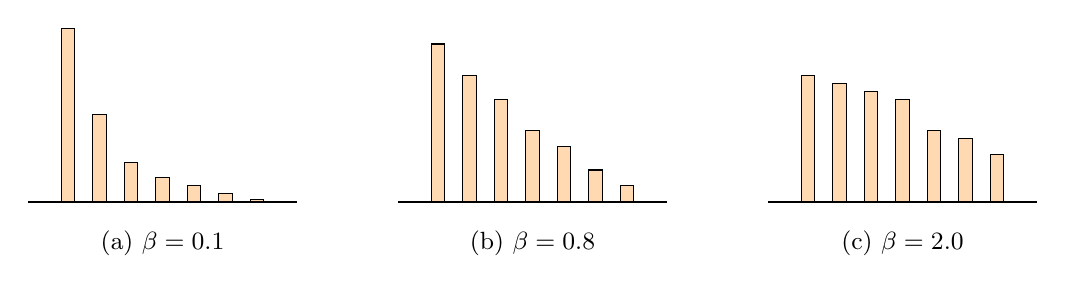
\begin{tikzpicture}
	
\def\ssep{0.4cm}
\def\wbias{0.6cm}
\def\sshift{1.85in}

\tikzstyle{pnode} = [minimum width=0.5em,inner sep=0pt,draw,rounded corners=0pt,fill=orange!30]

\begin{scope}[xshift=0em]

\node [anchor=south,pnode,minimum height=2.2cm] (p1) at (0,0) {};
\node [anchor=south,pnode,minimum height=1.1cm] (p2) at ([xshift=\ssep]p1.south) {};
\node [anchor=south,pnode,minimum height=0.5cm] (p3) at ([xshift=\ssep]p2.south) {};
\node [anchor=south,pnode,minimum height=0.3cm] (p4) at ([xshift=\ssep]p3.south) {};
\node [anchor=south,pnode,minimum height=0.2cm] (p5) at ([xshift=\ssep]p4.south) {};
\node [anchor=south,pnode,minimum height=0.1cm] (p6) at ([xshift=\ssep]p5.south) {};
\node [anchor=south,pnode,minimum height=0.03cm] (p7) at ([xshift=\ssep]p6.south) {};

\draw [-] ([xshift=-\wbias]p1.south east) -- ([xshift=\wbias]p7.south west);

\node [anchor=center] (label) at ([xshift=0,yshift=-\ssep*1.3]p4.south) {\small (a) $\beta=0.1$};

\end{scope}

\begin{scope}[xshift=\sshift]

\node [anchor=south,pnode,minimum height=2.0cm] (p1) at (0,0) {};
\node [anchor=south,pnode,minimum height=1.6cm] (p2) at ([xshift=\ssep]p1.south) {};
\node [anchor=south,pnode,minimum height=1.3cm] (p3) at ([xshift=\ssep]p2.south) {};
\node [anchor=south,pnode,minimum height=0.9cm] (p4) at ([xshift=\ssep]p3.south) {};
\node [anchor=south,pnode,minimum height=0.7cm] (p5) at ([xshift=\ssep]p4.south) {};
\node [anchor=south,pnode,minimum height=0.4cm] (p6) at ([xshift=\ssep]p5.south) {};
\node [anchor=south,pnode,minimum height=0.2cm] (p7) at ([xshift=\ssep]p6.south) {};

\draw [-] ([xshift=-\wbias]p1.south east) -- ([xshift=\wbias]p7.south west);

\node [anchor=center] (label) at ([xshift=0,yshift=-\ssep*1.3]p4.south) {\small (b) $\beta=0.8$};

\end{scope}

\begin{scope}[xshift=\sshift*2]

\node [anchor=south,pnode,minimum height=1.6cm] (p1) at (0,0) {};
\node [anchor=south,pnode,minimum height=1.5cm] (p2) at ([xshift=\ssep]p1.south) {};
\node [anchor=south,pnode,minimum height=1.4cm] (p3) at ([xshift=\ssep]p2.south) {};
\node [anchor=south,pnode,minimum height=1.3cm] (p4) at ([xshift=\ssep]p3.south) {};
\node [anchor=south,pnode,minimum height=0.9cm] (p5) at ([xshift=\ssep]p4.south) {};
\node [anchor=south,pnode,minimum height=0.8cm] (p6) at ([xshift=\ssep]p5.south) {};
\node [anchor=south,pnode,minimum height=0.6cm] (p7) at ([xshift=\ssep]p6.south) {};

\draw [-] ([xshift=-\wbias]p1.south east) -- ([xshift=\wbias]p7.south west);

\node [anchor=center] (label) at ([xshift=0,yshift=-\ssep*1.3]p4.south) {\small (c) $\beta=2.0$};

\end{scope}

\end{tikzpicture}
\end{center}

\vspace{-0.5cm} \caption{Histogram estimates of the distributions generated by the Softmax function with different values of the temperature parameter $\beta$.}
\label{fig:llm-softmax-with-temperature}
\end{figure}


\subsubsection{Decoding with Penalty Terms}

One common improvement to decoding methods in text generation is to modify the search objective. For example, one can replace maximum a posteriori (MAP) decoding with minimum Bayes risk (MBR) decoding~\cite{kumar-etal:2004minimum}, where the focus shifts from selecting the single most probable output to choosing an output that minimizes the expected risk over a distribution of possible outputs. Here we explore methods that incorporate penalty terms into decoding. These methods offer a simple but effective way to make decoding more controllable.

Recall from Eq. (\ref{eq:llm-general-decoding-objective}) that the goal of decoding is to maximize the likelihood of the output sequence. With penalty terms, the objective is extended to include additional factors that penalize certain behaviors in the generated text. A general form of the new objective is given by:
\begin{eqnarray}
\hat{\mathbf{y}} & = & \argmax_{\mathbf{y} \in \mathcal{Y}} \big[ \log \Pr(\mathbf{y}|\mathbf{x}) - \lambda \cdot \mathrm{Penalty}(\mathbf{x},\mathbf{y}) \big], \label{eq:llm-decoding-objective-with-penalty}
\end{eqnarray}

\noindent where $\mathrm{Penalty}(\mathbf{x},\mathbf{y})$ is a function that quantifies the degree to which the generated sequence $\mathbf{y}$ violates certain constraints or exhibits undesirable behaviors given the input $\mathbf{x}$. The design of $\mathrm{Penalty}(\cdot)$ is very flexible, thus allowing us to incorporate a wide range of constraints or prior knowledge into it. Below, we present some common types of penalty functions.

\begin{itemize}
\item \vspace{0.5em} \textbf{Repetition Penalty}. A repetition penalty discourages the model from generating repetitive or redundant text. The penalty function might measure the frequency of repeated tokens or phrases in the generated sequence and impose a penalty proportional to their occurrence.
\item \vspace{0.3em} \textbf{Length Penalty}. A length penalty ensures that the generated sequence adheres to a desired length. For example, in text summarization tasks, the penalty function could penalize outputs that are too short or too long.
\item \vspace{0.3em} \textbf{Diversity Penalty}. A diversity penalty promotes variation in the generated text. For example, in beam search, we can measure the similarity between generated hypotheses, and encourage the model to explore different hypotheses.
\item \vspace{0.3em} \textbf{Constraint-based Penalty}. A constraint-based penalty enforces specific constraints related to the content or style of the generated text. For example, in machine translation, the penalty function could penalize outputs that deviate from a desired tone or terminology.
\end{itemize}
\vspace{0.5em}

In general, we can consider $\mathrm{Penalty}(\mathbf{x},\mathbf{y})$ as a function that defines the cost assigned to the generated sequence $\mathbf{y}$ given the input sequence $\mathbf{x}$. Alternatively, this function can be defined to assess the hidden states of an LLM when generating $\mathbf{y}$. For example, \citet{su-etal:2022contrastive} develop a penalty term that calculates the maximum distance between the representation of the predicted token and the representations of the previously generated tokens. Therefore, the search objective will penalize degenerate outputs, such as text with many repetitions.

The method described in Eq. (\ref{eq:llm-decoding-objective-with-penalty}) is general and can be easily adapted to different search algorithms. For example, in greedy search, we can keep the single sequence that maximizes $\log \Pr(\mathbf{y}|\mathbf{x}) - \lambda \cdot \mathrm{Penalty}(\mathbf{x},\mathbf{y})$ at each decoding step; in sampling-based search, we can rank and select the top-ranked sequences based on $\log \Pr(\mathbf{y}|\mathbf{x}) - \lambda \cdot \mathrm{Penalty}(\mathbf{x},\mathbf{y})$ to form the candidate pool.

\subsubsection{Speculative Decoding}

\mindex{Speculative decoding} stems from the concept of \mindex{speculative execution}, where a system makes educated guesses about future actions and performs them in advance. If the guess is correct, the results are immediately available, which speeds up processing. In the case of LLM inference, suppose we have two models. One is a smaller, faster model (called the draft model), and the other is the full, stronger model (called the verification model). These two models represent two ends of the spectrum in LLM inference: the draft model is efficient but not very accurate; the verification model is usually the one we want to run, but it is very slow. Given a prefix, we first use the draft model to speculatively predict a sequence of likely future tokens. This is a standard autoregressive decoding process, but it is still fast in practice due to the high efficiency of the draft model. Then, the verification model evaluates the speculated tokens in parallel. It checks whether the predicted tokens can be accepted under the verification model. Note that, since we can deal with these tokens all at once, the verification can be done in a single step for all the tokens simultaneously, rather than in a token-by-token manner. If the speculated tokens are correct, they are accepted, and the process continues with the next set of tokens. If they are incorrect, the incorrect speculations are discarded, and the verification model is used to generate new tokens.

To be more specific, let us see the speculative decoding method presented in \citet{leviathan-etal:2023fast}'s work. In this method, the draft model is a small language model, denoted by $\Pr_q(y_i|\mathbf{x},\mathbf{y}_{<i})$, while the verification model is the full LLM, denoted by $\Pr_p(y_i|\mathbf{x},\mathbf{y}_{<i})$. The goal is to use the draft model, given a prefix, to autoregressively predict up to $\tau$ tokens. The verification model is then employed to generate the last token at the point where speculative predictions are rejected. Figure~\ref{fig:speculative-decoding-one-step} illustrates one step in this decoding process. For simplicity, we describe the greedy version of speculative decoding.

\begin{figure}[!t]
\centering
% !Mode:: "TeX:UTF-8"
% !TEX encoding = UTF-8 Unicode

\begin{center}
\begin{tikzpicture}
	
\def\ssep{1.2cm}

\tikzstyle{lnode} = [minimum width=3.0cm,minimum height=0.6cm,inner sep=2pt,draw,fill=white,rounded corners=0pt];
\tikzstyle{snode} = [minimum width=0.27cm,minimum height=0.18cm,inner sep=2pt,draw,fill=white];

% predictions made by the draft model
\begin{scope}

\node [lnode,anchor=west] (context) at (0,0) {\small{Context ($\mathbf{x}, \mathbf{y}_{<i}$)}};

\node [anchor=center] (y1) at ([xshift=1.5*\ssep]context.east) {\color{blue} \small{$\hat{y}_{i+1}$}};
\node [anchor=center] (y2) at ([xshift=\ssep]y1.center) {\color{blue} \small{$\hat{y}_{i+2}$}};
\node [anchor=center] (y3) at ([xshift=\ssep]y2.center) {\color{blue} \small{$\hat{y}_{i+3}$}};
\node [anchor=center] (y4) at ([xshift=\ssep]y3.center) {\color{blue} \small{$\hat{y}_{i+4}$}};
\node [anchor=center] (y5) at ([xshift=\ssep]y4.center) {\color{blue} \small{$\hat{y}_{i+5}$}};

\draw [->,double] ([xshift=3pt]context.east) -- ([xshift=-4pt]y1.west);

\draw [-] ([yshift=-0.3cm]y1.west) -- ([yshift=-0.3cm]y5.east);

\node [anchor=north,minimum width=5.7cm,minimum height=0.7cm,draw,thick] (draftmodel) at ([yshift=-0.5cm]y3.south) {\small{Draft Model $\mathrm{Pr}_q(\cdot)$}};
\draw [->,thick] ([yshift=2pt]draftmodel.north) -- ([yshift=0.4cm]draftmodel.north) node [pos=0.5,right,xshift=0.2cm] (predictlable) {\scriptsize{predict}};

\node [anchor=north] (caption) at ([yshift=-0.3cm,xshift=1cm]draftmodel.south west) {\small{(a) Predict the next $\tau$ tokens given the context using the draft model ($\tau = 5$)}};

\end{scope}

% evaluation by the evaluation model
\begin{scope}[yshift=-5cm]

\node [lnode,anchor=west] (context) at (0,0) {\small{Context ($\mathbf{x}, \mathbf{y}_{<i}$)}};

\node [anchor=center] (y1) at ([xshift=1.5*\ssep]context.east) {\color{blue} \small{$\hat{y}_{i+1}$}};
\node [anchor=center] (y2) at ([xshift=\ssep]y1.center) {\color{blue} \small{$\hat{y}_{i+2}$}};
\node [anchor=center] (y3) at ([xshift=\ssep]y2.center) {\color{blue} \small{$\hat{y}_{i+3}$}};
\node [anchor=center] (y4) at ([xshift=\ssep]y3.center) {\color{blue} \small{$\hat{y}_{i+4}$}};
\node [anchor=center] (y5) at ([xshift=\ssep]y4.center) {\color{blue} \small{$\hat{y}_{i+5}$}};

\draw [->,double] ([xshift=3pt]context.east) -- ([xshift=-4pt]y1.west);

%\draw [-] ([yshift=-0.3cm]y1.west) -- ([yshift=-0.3cm]y5.east);

\node [anchor=north,minimum width=5.7cm,minimum height=0.7cm,draw=gray!30,thick] (draftmodel) at ([yshift=-0.5cm]y3.south) {\color{gray!30} \small{Draft Model $\mathrm{Pr}_q(\cdot)$}};
\draw [->,thick,white] ([yshift=2pt]draftmodel.north) -- ([yshift=0.4cm]draftmodel.north);

\node [anchor=south,minimum width=5.7cm,minimum height=0.7cm,draw,thick] (evalmodel) at ([yshift=0.5cm]y3.north) {\small{Evaluation Model $\mathrm{Pr}_p(\cdot)$}};
\draw [->,thick] ([yshift=-2pt]evalmodel.south) -- ([yshift=-0.4cm]evalmodel.south) node [pos=0.5,right,xshift=0.2cm] (evaluatelable) {\scriptsize{evaluate}};

\begin{pgfonlayer}{background}
\node [draw,dotted,very thick,inner sep=1pt] [fit = (y1) (y5)] (predictionbox) {};
\end{pgfonlayer}

\node [anchor=north] (caption) at ([yshift=-0.3cm,xshift=1cm]draftmodel.south west) {\small{(b) Evaluate the predicted tokens using the evaluation model}};

\end{scope}

% determining accepted guesses
\begin{scope}[yshift=-10cm]

\node [lnode,anchor=west] (context) at (0,0) {\small{Context ($\mathbf{x}, \mathbf{y}_{<i}$)}};

\node [anchor=center] (y1) at ([xshift=1.5*\ssep]context.east) {\color{blue} \small{$\hat{y}_{i+1}$}};
\node [anchor=center] (y2) at ([xshift=\ssep]y1.center) {\color{blue} \small{$\hat{y}_{i+2}$}};
\node [anchor=center] (y3) at ([xshift=\ssep]y2.center) {\color{blue} \small{$\hat{y}_{i+3}$}};
\node [anchor=center] (y4) at ([xshift=\ssep]y3.center) {\color{blue} \small{$\hat{y}_{i+4}$}};
\node [anchor=center] (y5) at ([xshift=\ssep]y4.center) {\color{blue} \small{$\hat{y}_{i+5}$}};

\draw [->,double] ([xshift=3pt]context.east) -- ([xshift=-4pt]y1.west);

%\draw [-] ([yshift=-0.3cm]y1.west) -- ([yshift=-0.3cm]y5.east);

\node [anchor=north,minimum width=5.7cm,minimum height=0.7cm,draw=gray!30,thick] (draftmodel) at ([yshift=-0.5cm]y3.south) {\color{gray!30} \small{Draft Model $\mathrm{Pr}_q(\cdot)$}};
\draw [->,thick,white] ([yshift=2pt]draftmodel.north) -- ([yshift=0.4cm]draftmodel.north);

\node [anchor=south,minimum width=5.7cm,minimum height=0.7cm,draw=gray!30,thick] (evalmodel) at ([yshift=0.5cm]y3.north) {\color{gray!30} \small{Evaluation Model $\mathrm{Pr}_p(\cdot)$}};
\draw [->,thick,white] ([yshift=-2pt]evalmodel.south) -- ([yshift=-0.4cm]evalmodel.south);

\begin{pgfonlayer}{background}
\node [draw=blue,dotted,very thick,inner sep=1pt] [fit = (y1) (y3)] (predictionbox) {};
\node [draw=red,dotted,very thick,inner sep=1pt] [fit = (y4) (y5)] (predictionbox2) {};
\end{pgfonlayer}

\node [anchor=south] (acceptedlabel) at (predictionbox.north) {\color{blue} \scriptsize{accepted}};
\node [anchor=south] (rejectedlabel) at (predictionbox2.north) {\color{red} \scriptsize{rejected}};
\draw [-,red] ([yshift=-2pt,xshift=3pt]predictionbox2.north west) -- ([yshift=2pt,xshift=-3pt]predictionbox2.south east);
\draw [-,red] ([yshift=-2pt,xshift=-3pt]predictionbox2.north east) -- ([yshift=2pt,xshift=3pt]predictionbox2.south west);

\node [anchor=north] (caption) at ([yshift=-0.3cm,xshift=1cm]draftmodel.south west) {\small{(c) Determine the number of accepted tokens}};

\end{scope}

% predicting a new token
\begin{scope}[yshift=-15cm]

\node [lnode,anchor=west] (context) at (0,0) {\small{Context ($\mathbf{x}, \mathbf{y}_{<i}$)}};

\node [anchor=center] (y1) at ([xshift=1.5*\ssep]context.east) {\color{blue} \small{$\hat{y}_{i+1}$}};
\node [anchor=center] (y2) at ([xshift=\ssep]y1.center) {\color{blue} \small{$\hat{y}_{i+2}$}};
\node [anchor=center] (y3) at ([xshift=\ssep]y2.center) {\color{blue} \small{$\hat{y}_{i+3}$}};
\node [anchor=center,fill=gray!30] (y4) at ([xshift=\ssep]y3.center) {\color{black} \small{$\bar{y}_{i+4}$}};

\draw [->,double] ([xshift=3pt]context.east) -- ([xshift=-4pt]y1.west);

%\draw [-] ([yshift=-0.3cm]y1.west) -- ([yshift=-0.3cm]y5.east);
\draw [<-,thick] ([yshift=2pt]y4.north) -- ([yshift=0.45cm]y4.north);

\node [anchor=north,minimum width=5.7cm,minimum height=0.7cm,draw=gray!30,thick] (draftmodel) at ([yshift=-0.5cm]y3.south) {\color{gray!30} \small{Draft Model $\mathrm{Pr}_q(\cdot)$}};
\draw [->,thick,white] ([yshift=2pt]draftmodel.north) -- ([yshift=0.4cm]draftmodel.north);

\node [anchor=south,minimum width=5.7cm,minimum height=0.7cm,draw,thick] (evalmodel) at ([yshift=0.5cm]y3.north) {\small{Evaluation Model $\mathrm{Pr}_p(\cdot)$}};
\draw [->,thick,white] ([yshift=-2pt]evalmodel.south) -- ([yshift=-0.4cm]evalmodel.south);

\node [anchor=north] (caption) at ([yshift=-0.3cm,xshift=1cm]draftmodel.south west) {\small{(d) Predict a new token following the accepted tokens using the evaluation model}};

\end{scope}

\end{tikzpicture}
\end{center}

\vspace{-0.5cm} \caption{Illustration of one step of speculative decoding. The goal is to predict as many next tokens as possible using the draft model. There are four sub-steps. Given the context, we first use the draft model to predict the next $\tau$ tokens. Then, we evaluate these predictions in parallel using the verification model. Next, we determine the maximum number of predicted tokens that can be accepted. Finally, we use the evaluation model to predict a new token following these accepted tokens.}
\label{fig:speculative-decoding-one-step}
\end{figure}

The speculative decoding algorithm can be summarized as follows.

\begin{itemize}
\item \vspace{0.5em} Given the prefix $[\mathbf{x},\mathbf{y}_{\le i}]$, we use the draft model to predict the next $\tau$ consecutive tokens, denoted by $\{\hat{y}_{i+1},\cdots,\hat{y}_{i+\tau}\}$. This is a token-by-token generation process, given by:
    \begin{eqnarray}
    \hat{y}_{i+t} & = & \argmax_{y_{i+t}} \mathrm{Pr}_q(y_{i+t}|\mathbf{x},\mathbf{y}_{\le i},\hat{y}_{i+1}\cdots\hat{y}_{i+t-1}).
    \end{eqnarray}
\item \vspace{0.3em} We evaluate $\{\hat{y}_{i+1},\cdots,\hat{y}_{i+\tau}\}$ using the verification model, that is, we compute $\{\mathrm{Pr}_p(\hat{y}_{i+1}|\mathbf{x},\mathbf{y}_{\le i})$ $,\cdots,\mathrm{Pr}_p(\hat{y}_{i+\tau}|\mathbf{x},\mathbf{y}_{\le i},\hat{y}_{i+1}\cdots\hat{y}_{i+\tau-1})\}$. Note that we can compute these probabilities in parallel, and so this verification step is efficient.
\item \vspace{0.3em} We determine the maximum number of accepted speculated tokens. To keep the notation uncluttered, we denote $\mathrm{Pr}_q(\hat{y}_{i+t}|\mathbf{x},\mathbf{y}_{\le i},\hat{y}_{i+1}\cdots\hat{y}_{i+t-1})$ and $\mathrm{Pr}_p(\hat{y}_{i+t}|\mathbf{x},\mathbf{y}_{\le i},\hat{y}_{i+1}\cdots\hat{y}_{i+t-1})$ simply by $q(\hat{y}_{i+t})$ and $p(\hat{y}_{i+t})$, respectively. We then define the acceptance rule as follows: if $q(\hat{y}_{i+t}) \le p(\hat{y}_{i+t})$, then we accept this speculation. By contrast, if $q(\hat{y}_{i+t}) > p(\hat{y}_{i+t})$, we reject this speculation with probability $1-\frac{p(\hat{y}_{i+t})}{q(\hat{y}_{i+t})}$. Starting from $\hat{y}_{i+1}$, the maximum number of accepted consecutive speculated tokens is defined as:
    \begin{eqnarray}
    n_a & = & \min \left\{t-1 | 1 \le t \le \tau, r_t > \frac{p(\hat{y}_{i+t})}{q(\hat{y}_{i+t})} \right\},
    \end{eqnarray}
    \noindent where $r_t$ is a variable drawn from the uniform distribution $U(0,1)$. If all speculative tokens are accepted, we set $n_a=\tau$.
\item Given $n_a$, we keep the speculated tokens $\{\hat{y}_{i+1},\cdots,\hat{y}_{i+n_a}\}$. We then use the verification model to make a new prediction at $i+n_a+1$:
    \begin{eqnarray}
    \bar{y}_{i+n_a+1} & = & \argmax_{y_{i+n_a+1}} \mathrm{Pr}_p(y_{i+n_a+1}|\mathbf{x},\mathbf{y}_{\le i},\hat{y}_{i+1}\cdots\hat{y}_{i+n_a}).
    \end{eqnarray}
\item Above, we have described one step of speculative decoding. The result sequence (including both the context and predicted tokens) is illustrated as follows
\begin{center}
% !Mode:: "TeX:UTF-8"
% !TEX encoding = UTF-8 Unicode

\begin{center}
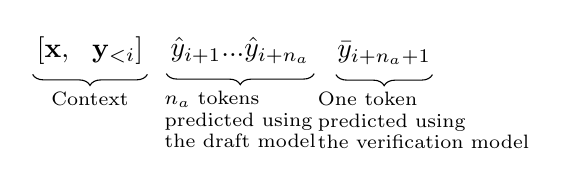
\begin{tikzpicture}
	
\def\ssep{0.8cm}
\def\nodew{10cm}

\tikzstyle{lnode} = [minimum width=3cm,minimum height=1.0cm,inner sep=2pt,draw,thick,fill=white,rounded corners=1pt];
\tikzstyle{snode} = [circle,minimum size=0.2cm,inner sep=0,draw=white,line width=0.02cm,fill=black];

\begin{scope}

\node[anchor=west] (s1) at (0,0) {$[\mathbf{x},\ \ \mathbf{y}_{<i}]$};
\node[anchor=west] (s2) at ([xshift=0.1cm]s1.east) {$\hat{y}_{i+1} ... \hat{y}_{i+n_a}$};
\node[anchor=west] (s3) at ([xshift=0.1cm,yshift=-1pt]s2.east) {$\bar{y}_{i+n_a+1}$};

\draw [decoration={brace,amplitude=4pt},decorate] ([yshift=-0.0cm,xshift=-2pt]s1.south east) -- ([yshift=-0.0cm,xshift=2pt]s1.south west) node [pos=0.5,below,yshift=-0.1cm] {\scriptsize{Context}};
\draw [decoration={brace,amplitude=4pt},decorate] ([yshift=-0.0cm,xshift=-2pt]s2.south east) -- ([yshift=-0.0cm,xshift=2pt]s2.south west) node [pos=0.5,below,yshift=-0.1cm,align=left] {\scriptsize{$n_a$ tokens}\\[-0.15cm] \scriptsize{predicted using}\\[-0.15cm] \scriptsize{the draft model}};
\draw [decoration={brace,amplitude=4pt},decorate] ([yshift=-0.0cm,xshift=-3pt]s3.south east) -- ([yshift=-0.0cm,xshift=3pt]s3.south west) node [pos=0.5,below,yshift=-0.1cm,xshift=0.5cm,align=left] {\scriptsize{One token}\\[-0.15cm] \scriptsize{predicted using}\\[-0.15cm] \scriptsize{the verification model}};

\end{scope}

\end{tikzpicture}
\end{center}

\end{center}
    Once we have finished this step, we add the predicted tokens $\{\hat{y}_{i+1},\cdots,\hat{y}_{i+n_a},\bar{y}_{i+n_a+1} \}$ to the context, and repeat the above process.
\end{itemize}
\vspace{0.5em}

In practice, we usually wish to use a smaller draft model so that predicting $\{\hat{y}_{i+1},\cdots,\hat{y}_{i+n_a}\}$ would be computationally cheaper. But a very small draft model is less accurate and can result in smaller $n_a$. We therefore need to carefully select the draft model to make the trade-off between the computational efficiency and accuracy.

\subsubsection{Stopping Criteria}

Stopping criteria are a critical component of LLM inference. They typically involve rules or conditions that specify when the model should stop generating text during decoding. Most LLMs are trained to generate an end-of-sequence token (e.g., $\langle \mathrm{EOS} \rangle$ or $\langle /s \rangle$) to signal the end of the generated text. Thus, the simplest strategy is to halt the generation process when this token is produced. For beam search, which explores multiple hypotheses simultaneously, the process can continue until a given number of complete sequences have been generated.

In practical applications, it will generally be undesirable to generate very long sequences, and so we need to reduce the decoding cost and unnecessary verbosity. One commonly used stopping criterion is the maximum length of the output. The model stops generating text once it has produced a predetermined number of tokens. Alternatively, we can stop the decoding based on actual computational cost, such as the computational resources or time constraints. For example, in real-time applications like chatbots, decoding may need to stop after a certain time limit to ensure responsiveness.

Another approach is to design stopping criteria based on the behavior of LLMs. For example, decoding can be stopped if the probability of predicting the next token falls below a certain threshold. In addition to probability-based stopping, a repetition detection module can be implemented to trigger the model to stop if it begins repeating tokens or phrases beyond a predefined limit. This helps prevent redundant or incoherent outputs.

\subsection{Evaluation Metrics for LLM Inference}

Evaluating the performance of LLM inference systems involves a variety of metrics to assess how well these models meet desired standards, such as quality, robustness, usability, and efficiency. As with most NLP systems, we can evaluate LLMs using standard NLP evaluation metrics, such as perplexity and F1 score. We can also examine their robustness by testing how well they handle ambiguous or challenging inputs, including adversarial examples, perturbed inputs, and out-of-distribution data. Additionally, usability can be assessed by measuring how well the generated outputs align with user expectations in terms of fluency, coherence, relevance, and diversity. Human evaluators can rate the naturalness of the text or assess whether the responses are contextually appropriate and logically consistent. Ethical and fairness metrics can also be included to ensure LLMs avoid perpetuating biases or generating harmful content.

All of the evaluation metrics mentioned above focus primarily on assessing the quality of the outputs. Given the high cost of deploying and serving LLMs, efficiency metrics are also very important for practitioners. Below are some commonly used efficiency metrics~\cite{nvidia-nim-llm-benchmarking}:

\begin{itemize}
\item \vspace{0.5em} \textbf{Request Latency}. This metric measures the total time taken from when a request is sent to the LLM until the complete response is received. This includes the time taken for data transmission, processing by the model, and the return of the output to the user.
\item \vspace{0.3em} \textbf{Throughput}. This metric measures the number of requests or generated tokens that the system can process per unit time. Throughput is commonly reported as requests per second (RPS) or tokens per second (TPS).
\item \vspace{0.3em} \textbf{Time to First Token} (TTFT). This metric measures the time between sending a request and generating the first token of the response. If data transmission does not consume too much time, then TTFT mainly consists of the time required for the prefilling stage and the generation of the first token.
\item \vspace{0.3em} \textbf{Inter-token Latency} (ITL). This metric refers to the time taken to generate each subsequent token after the first one. It reflects the efficiency of the decoding process.
\item \vspace{0.3em} \textbf{Resource Utilization}. This involves measuring the computational resource usage (e.g., CPU and GPU utilization) and memory consumption of the model during inference.
\end{itemize}
\vspace{0.5em}

In addition to these metrics, energy efficiency and cost efficiency are practical considerations for deploying LLMs at scale. Energy efficiency measures the amount of electrical power consumed by the model during inference. Cost efficiency, on the other hand, evaluates the total expenses related to deploying and maintaining the model.

In general, choosing the right evaluation metrics depends on the specific task and application. While quality-focused metrics are essential for assessing LLMs, efficiency metrics are equally crucial for their effective deployment in real-world applications. A comprehensive evaluation framework should include both sets of metrics to accurately measure an LLM's performance and practicality.

%----------------------------------------------------------------------------------------
% NEW SECTION
%----------------------------------------------------------------------------------------

\section{Efficient Inference Techniques}

In practical applications, we often wish a system to be as efficient as possible. For LLM inference, this typically involves two types of improvements: reducing memory requirements and accelerating inference. For example, we can modify the Transformer architecture to avoid memory explosion when processing very long input sequences. Another example is that we can compress input sequences to reduce computational overhead while preserving their semantic information. In addition, techniques like quantization and pruning can be employed to further optimize memory usage and inference speed.

Efficient inference is a wide-ranging topic that overlaps with several areas of LLM research, such as architecture design and model compression. Most of these topics have been covered in previous chapters. For example, in Chapter \ChapterLLM, we discussed long-context LLMs; and in Chapter \ChapterLLMPrompting, we discussed prompt compression methods for reducing prompt length. In this section, we focus on techniques that are commonly used in LLM deployment and serving.

\subsection{Prefix Caching}

In real-world applications, it is common to cache frequent requests and their corresponding responses. When a new request hits the cache, the system can retrieve the response directly from the cache instead of recomputing the result. One straightforward implementation is a key-value datastore (e.g., a hash table) that maps input sequences to their LLM-generated output sequences. In the simplest case, we can collect frequent queries, generate their responses using the LLM, and store these query-response pairs in the datastore. This creates a basic sequence-level caching mechanism that allows the system to bypass LLM computation when the input sequence exactly matches a cached query.

A straightforward extension of the caching mechanism is to cache prefixes and their corresponding KV cache states. Given an input sequence $\mathbf{x}$ in a dataset $\mathcal{D}$, we can process it as in the standard prefilling phase. This produces a sequence of prefixes and their corresponding KV cache states:
\begin{eqnarray}
x_0\ (\text{i.e., } \mathbf{x}_{<1}) & \Rightarrow & \mathrm{cache}_{<1} \nonumber \\
x_0 x_1\ (\text{i.e., } \mathbf{x}_{<2}) & \Rightarrow & \mathrm{cache}_{<2} \nonumber \\
& \cdots & \nonumber \\
x_0 x_1 \cdots x_{m-1}\ (\text{i.e., } \mathbf{x}_{<m}) & \Rightarrow & \mathrm{cache}_{<m} \nonumber
\end{eqnarray}

\noindent where $\mathrm{cache}_{<i}$ denotes the KV cache for the prefix $\mathbf{x}_{<i}$ (see also Eq. (\ref{eq:prefilling-kv-cache})). All these mappings can be stored in the prefix cache for efficient reuse.

When processing a new sequence that shares a common prefix with a previously seen sequence in $\mathcal{D}$, we can load the corresponding cached KV states instead of recomputing them. Specifically, if a new input $\mathbf{x}'$ shares a prefix $\mathbf{x}_{<k}$ with an existing sequence (i.e., $\mathbf{x}'_{<k} = \mathbf{x}_{<k}$ for some $k \le m$), we can initialize the KV cache with $\mathrm{cache}_{<k}$ and only compute the KV states for the remaining tokens $\mathbf{x}'_{\ge k}$.

As usual, we can maintain a key-value datastore that maps frequently encountered prefixes to their precomputed KV caches. The lookup can be performed using a hash of the prefix tokens, allowing constant-time access to the cached states. Care must be taken to manage memory usage, as storing all possible prefixes may be infeasible for large datasets. Practical systems often employ least recently used (LRU) caching methods or other strategies to balance between computational savings and memory constraints.

\subsection{Batching}

Batching in LLM inference refers to processing multiple input sequences simultaneously as a group (called a batch) rather than one at a time. Because modern GPUs excel at parallel processing, batching allows them to compute multiple sequences in a single forward pass, keeping the hardware fully occupied. Therefore, when serving LLMs at scale, batching is important for improving computational efficiency and maximizing hardware utilization\footnote{See \url{https://docs.nvidia.com/deeplearning/performance/dl-performance-gpu-background/index.html\#understand-perf} for a simple evaluation.}.

To illustrate the idea of batching, Figure~\ref{fig:basic-llm-batching-methods} (a-b) shows simple examples with batch sizes of 1 and 4, respectively. When using a batch size of 1 (i.e., without batching), the GPU processes one input sequence at a time. Thus, the processing is sequential: the next sequence must wait for the current computation to finish. By contrast, when using a batch size of 4, the GPU can process four sequences simultaneously in a single forward pass. As the input sequences vary in length, we need to standardize their length using padding techniques. Here we use left padding, which adds dummy tokens to the beginnings of short sequences, so that all sequences in the batch have the same length in prefilling. For decoding, tokens are generated simultaneously for all these sequences, and generation continues until all sequences in the batch finish decoding.

\begin{figure}[!t]
\centering
% !Mode:: "TeX:UTF-8"
% !TEX encoding = UTF-8 Unicode

\begin{center}
\begin{tikzpicture}
	
\def\ssep{0.12cm}

\tikzstyle{lnode} = [minimum width=3.0cm,minimum height=0.6cm,inner sep=2pt,draw,fill=white,rounded corners=0pt];
\tikzstyle{snode} = [minimum width=0.33cm,minimum height=0.33cm,inner sep=0pt,draw,fill=white];

% inference (batch size = 1)
\begin{scope}

\node [snode,anchor=west,fill=red!30] (x00) at (0,0) {};
\node [snode,anchor=east,fill=red!30] (x01) at ([xshift=-\ssep]x00.west) {};
\node [snode,anchor=east,fill=red!30] (x02) at ([xshift=-\ssep]x01.west) {};
\node [snode,anchor=east,fill=red!30] (x03) at ([xshift=-\ssep]x02.west) {};
\node [snode,anchor=east,fill=red!30] (x04) at ([xshift=-\ssep]x03.west) {};

\node [snode,anchor=west,fill=blue!30] (y01) at ([xshift=2*\ssep]x00.east) {};
\node [snode,anchor=west,fill=blue!30] (y02) at ([xshift=\ssep]y01.east) {};
\node [snode,anchor=west,fill=blue!30] (y03) at ([xshift=\ssep]y02.east) {};
\node [snode,anchor=west,fill=blue!30] (y04) at ([xshift=\ssep]y03.east) {};

\draw [decoration={brace,amplitude=4pt},decorate] ([yshift=0.1cm,xshift=0.0cm]x04.north west) -- ([yshift=0.1cm,xshift=0.0cm]x00.north east) node [above,pos=0.5,yshift=0.1cm] {\scriptsize{prefilling}};
\draw [decoration={brace,amplitude=4pt},decorate] ([yshift=0.1cm,xshift=0.0cm]y01.north west) -- ([yshift=0.1cm,xshift=0.0cm]y04.north east) node [above,pos=0.5,yshift=0.1cm] {\scriptsize{decoding}};

\node [anchor=north] (caption) at ([yshift=-2cm]x00.south east) {\footnotesize{(a) batch size $= 1$}};

\end{scope}

% inference (batch size = 4)
\begin{scope}[xshift=7.5cm]

\node [snode,anchor=west,fill=red!30] (x00) at (0,0) {\scriptsize{1}};
\node [snode,anchor=east,fill=red!30] (x01) at ([xshift=-\ssep]x00.west) {\scriptsize{1}};
\node [snode,anchor=east,fill=red!30] (x02) at ([xshift=-\ssep]x01.west) {\scriptsize{1}};
\node [snode,anchor=east,fill=red!30] (x03) at ([xshift=-\ssep]x02.west) {\scriptsize{1}};
\node [snode,anchor=east,fill=red!30] (x04) at ([xshift=-\ssep]x03.west) {\scriptsize{1}};
\node [snode,anchor=east,fill=ugreen!30] (x05) at ([xshift=-\ssep]x04.west) {\tiny{pad}};

\node [snode,anchor=west,fill=blue!30] (y01) at ([xshift=2*\ssep]x00.east) {\scriptsize{1}};
\node [snode,anchor=west,fill=blue!30] (y02) at ([xshift=\ssep]y01.east) {\scriptsize{1}};
\node [snode,anchor=west,fill=blue!30] (y03) at ([xshift=\ssep]y02.east) {\scriptsize{1}};
\node [snode,anchor=west,fill=blue!30] (y04) at ([xshift=\ssep]y03.east) {\scriptsize{1}};
\node [snode,anchor=west,fill=gray!30] (y05) at ([xshift=\ssep]y04.east) {};
\node [snode,anchor=west,fill=gray!30] (y06) at ([xshift=\ssep]y05.east) {};

\node [snode,anchor=north,fill=red!30] (x10) at ([yshift=-\ssep]x00.south) {\scriptsize{2}};
\node [snode,anchor=east,fill=red!30] (x11) at ([xshift=-\ssep]x10.west) {\scriptsize{2}};
\node [snode,anchor=east,fill=red!30] (x12) at ([xshift=-\ssep]x11.west) {\scriptsize{2}};
\node [snode,anchor=east,fill=red!30] (x13) at ([xshift=-\ssep]x12.west) {\scriptsize{2}};
\node [snode,anchor=east,fill=ugreen!30] (x14) at ([xshift=-\ssep]x13.west) {\tiny{pad}};
\node [snode,anchor=east,fill=ugreen!30] (x15) at ([xshift=-\ssep]x14.west) {\tiny{pad}};

\node [snode,anchor=west,fill=blue!30] (y11) at ([xshift=2*\ssep]x10.east) {\scriptsize{2}};
\node [snode,anchor=west,fill=blue!30] (y12) at ([xshift=\ssep]y11.east) {\scriptsize{2}};
\node [snode,anchor=west,fill=blue!30] (y13) at ([xshift=\ssep]y12.east) {\scriptsize{2}};
\node [snode,anchor=west,fill=gray!30] (y14) at ([xshift=\ssep]y13.east) {};
\node [snode,anchor=west,fill=gray!30] (y15) at ([xshift=\ssep]y14.east) {};
\node [snode,anchor=west,fill=gray!30] (y16) at ([xshift=\ssep]y15.east) {};

\node [snode,anchor=north,fill=red!30] (x20) at ([yshift=-\ssep]x10.south) {\scriptsize{3}};
\node [snode,anchor=east,fill=red!30] (x21) at ([xshift=-\ssep]x20.west) {\scriptsize{3}};
\node [snode,anchor=east,fill=red!30] (x22) at ([xshift=-\ssep]x21.west) {\scriptsize{3}};
\node [snode,anchor=east,fill=ugreen!30] (x23) at ([xshift=-\ssep]x22.west) {\tiny{pad}};
\node [snode,anchor=east,fill=ugreen!30] (x24) at ([xshift=-\ssep]x23.west) {\tiny{pad}};
\node [snode,anchor=east,fill=ugreen!30] (x25) at ([xshift=-\ssep]x24.west) {\tiny{pad}};

\node [snode,anchor=west,fill=blue!30] (y21) at ([xshift=2*\ssep]x20.east) {\scriptsize{3}};
\node [snode,anchor=west,fill=blue!30] (y22) at ([xshift=\ssep]y21.east) {\scriptsize{3}};
\node [snode,anchor=west,fill=gray!30] (y23) at ([xshift=\ssep]y22.east) {};
\node [snode,anchor=west,fill=gray!30] (y24) at ([xshift=\ssep]y23.east) {};
\node [snode,anchor=west,fill=gray!30] (y25) at ([xshift=\ssep]y24.east) {};
\node [snode,anchor=west,fill=gray!30] (y26) at ([xshift=\ssep]y25.east) {};

\node [snode,anchor=north,fill=red!30] (x30) at ([yshift=-\ssep]x20.south) {\scriptsize{4}};
\node [snode,anchor=east,fill=red!30] (x31) at ([xshift=-\ssep]x30.west) {\scriptsize{4}};
\node [snode,anchor=east,fill=red!30] (x32) at ([xshift=-\ssep]x31.west) {\scriptsize{4}};
\node [snode,anchor=east,fill=red!30] (x33) at ([xshift=-\ssep]x32.west) {\scriptsize{4}};
\node [snode,anchor=east,fill=red!30] (x34) at ([xshift=-\ssep]x33.west) {\scriptsize{4}};
\node [snode,anchor=east,fill=red!30] (x35) at ([xshift=-\ssep]x34.west) {\scriptsize{4}};

\node [snode,anchor=west,fill=blue!30] (y31) at ([xshift=2*\ssep]x30.east) {\scriptsize{4}};
\node [snode,anchor=west,fill=blue!30] (y32) at ([xshift=\ssep]y31.east) {\scriptsize{4}};
\node [snode,anchor=west,fill=blue!30] (y33) at ([xshift=\ssep]y32.east) {\scriptsize{4}};
\node [snode,anchor=west,fill=blue!30] (y34) at ([xshift=\ssep]y33.east) {\scriptsize{4}};
\node [snode,anchor=west,fill=blue!30] (y35) at ([xshift=\ssep]y34.east) {\scriptsize{4}};
\node [snode,anchor=west,fill=blue!30] (y36) at ([xshift=\ssep]y35.east) {\scriptsize{4}};

\draw [decoration={brace,amplitude=4pt},decorate] ([yshift=0.1cm,xshift=0.0cm]x05.north west) -- ([yshift=0.1cm,xshift=0.0cm]x00.north east) node [above,pos=0.5,yshift=0.1cm] {\scriptsize{prefilling}};
\draw [decoration={brace,amplitude=4pt},decorate] ([yshift=0.1cm,xshift=0.0cm]y01.north west) -- ([yshift=0.1cm,xshift=0.0cm]y06.north east) node [above,pos=0.5,yshift=0.1cm] {\scriptsize{decoding}};

\node [anchor=north] (caption) at ([yshift=-2cm]x00.south east) {\footnotesize{(b) batch size $= 4$}};

\end{scope}

% inference (batch size = 4, sorted by length)
\begin{scope}[yshift=-5.3cm]

\node [snode,anchor=west,fill=red!30] (x00) at (0,0) {\scriptsize{1}};
\node [snode,anchor=east,fill=red!30] (x01) at ([xshift=-\ssep]x00.west) {\scriptsize{1}};
\node [snode,anchor=east,fill=red!30] (x02) at ([xshift=-\ssep]x01.west) {\scriptsize{1}};
\node [snode,anchor=east,fill=red!30] (x03) at ([xshift=-\ssep]x02.west) {\scriptsize{1}};
\node [snode,anchor=east,fill=red!30] (x04) at ([xshift=-\ssep]x03.west) {\scriptsize{1}};
\node [snode,anchor=east,fill=ugreen!30] (x05) at ([xshift=-\ssep]x04.west) {\tiny{pad}};

\node [snode,anchor=west,fill=blue!30] (y01) at ([xshift=2*\ssep]x00.east) {\scriptsize{1}};
\node [snode,anchor=west,fill=blue!30] (y02) at ([xshift=\ssep]y01.east) {\scriptsize{1}};
\node [snode,anchor=west,fill=blue!30] (y03) at ([xshift=\ssep]y02.east) {\scriptsize{1}};
\node [snode,anchor=west,fill=blue!30] (y04) at ([xshift=\ssep]y03.east) {\scriptsize{1}};
\node [snode,anchor=west,fill=blue!30] (y05) at ([xshift=\ssep]y04.east) {\scriptsize{1}};
\node [snode,anchor=west,fill=blue!30] (y06) at ([xshift=\ssep]y05.east) {\scriptsize{1}};

\node [snode,anchor=north,fill=red!30] (x10) at ([yshift=-\ssep]x00.south) {\scriptsize{2}};
\node [snode,anchor=east,fill=red!30] (x11) at ([xshift=-\ssep]x10.west) {\scriptsize{2}};
\node [snode,anchor=east,fill=red!30] (x12) at ([xshift=-\ssep]x11.west) {\scriptsize{2}};
\node [snode,anchor=east,fill=red!30] (x13) at ([xshift=-\ssep]x12.west) {\scriptsize{2}};
\node [snode,anchor=east,fill=red!30] (x14) at ([xshift=-\ssep]x13.west) {\scriptsize{2}};
\node [snode,anchor=east,fill=ugreen!30] (x15) at ([xshift=-\ssep]x14.west) {\tiny{pad}};

\node [snode,anchor=west,fill=blue!30] (y11) at ([xshift=2*\ssep]x10.east) {\scriptsize{2}};
\node [snode,anchor=west,fill=blue!30] (y12) at ([xshift=\ssep]y11.east) {\scriptsize{2}};
\node [snode,anchor=west,fill=blue!30] (y13) at ([xshift=\ssep]y12.east) {\scriptsize{2}};
\node [snode,anchor=west,fill=blue!30] (y14) at ([xshift=\ssep]y13.east) {\scriptsize{2}};
\node [snode,anchor=west,fill=blue!30] (y15) at ([xshift=\ssep]y14.east) {\scriptsize{2}};
\node [snode,anchor=west,fill=gray!30] (y16) at ([xshift=\ssep]y15.east) {};

\node [snode,anchor=north,fill=red!30] (x20) at ([yshift=-\ssep]x10.south) {\scriptsize{3}};
\node [snode,anchor=east,fill=red!30] (x21) at ([xshift=-\ssep]x20.west) {\scriptsize{3}};
\node [snode,anchor=east,fill=red!30] (x22) at ([xshift=-\ssep]x21.west) {\scriptsize{3}};
\node [snode,anchor=east,fill=red!30] (x23) at ([xshift=-\ssep]x22.west) {\scriptsize{3}};
\node [snode,anchor=east,fill=red!30] (x24) at ([xshift=-\ssep]x23.west) {\scriptsize{3}};
\node [snode,anchor=east,fill=red!30] (x25) at ([xshift=-\ssep]x24.west) {\scriptsize{3}};

\node [snode,anchor=west,fill=blue!30] (y21) at ([xshift=2*\ssep]x20.east) {\scriptsize{3}};
\node [snode,anchor=west,fill=blue!30] (y22) at ([xshift=\ssep]y21.east) {\scriptsize{3}};
\node [snode,anchor=west,fill=blue!30] (y23) at ([xshift=\ssep]y22.east) {\scriptsize{3}};
\node [snode,anchor=west,fill=blue!30] (y24) at ([xshift=\ssep]y23.east) {\scriptsize{3}};
\node [snode,anchor=west,fill=blue!30] (y25) at ([xshift=\ssep]y24.east) {\scriptsize{3}};
\node [snode,anchor=west,fill=gray!30] (y26) at ([xshift=\ssep]y25.east) {};

\node [snode,anchor=north,fill=red!30] (x30) at ([yshift=-\ssep]x20.south) {\scriptsize{4}};
\node [snode,anchor=east,fill=red!30] (x31) at ([xshift=-\ssep]x30.west) {\scriptsize{4}};
\node [snode,anchor=east,fill=red!30] (x32) at ([xshift=-\ssep]x31.west) {\scriptsize{4}};
\node [snode,anchor=east,fill=red!30] (x33) at ([xshift=-\ssep]x32.west) {\scriptsize{4}};
\node [snode,anchor=east,fill=red!30] (x34) at ([xshift=-\ssep]x33.west) {\scriptsize{4}};
\node [snode,anchor=east,fill=red!30] (x35) at ([xshift=-\ssep]x34.west) {\scriptsize{4}};

\node [snode,anchor=west,fill=blue!30] (y31) at ([xshift=2*\ssep]x30.east) {\scriptsize{4}};
\node [snode,anchor=west,fill=blue!30] (y32) at ([xshift=\ssep]y31.east) {\scriptsize{4}};
\node [snode,anchor=west,fill=blue!30] (y33) at ([xshift=\ssep]y32.east) {\scriptsize{4}};
\node [snode,anchor=west,fill=blue!30] (y34) at ([xshift=\ssep]y33.east) {\scriptsize{4}};
\node [snode,anchor=west,fill=blue!30] (y35) at ([xshift=\ssep]y34.east) {\scriptsize{4}};
\node [snode,anchor=west,fill=blue!30] (y36) at ([xshift=\ssep]y35.east) {\scriptsize{4}};

\draw [decoration={brace,amplitude=4pt},decorate] ([yshift=0.1cm,xshift=0.0cm]x05.north west) -- ([yshift=0.1cm,xshift=0.0cm]x00.north east) node [above,pos=0.5,yshift=0.1cm] {\scriptsize{prefilling}};
\draw [decoration={brace,amplitude=4pt},decorate] ([yshift=0.1cm,xshift=0.0cm]y01.north west) -- ([yshift=0.1cm,xshift=0.0cm]y06.north east) node [above,pos=0.5,yshift=0.1cm] {\scriptsize{decoding}};

\node [anchor=north] (caption) at ([yshift=-2.9cm,xshift=0.1cm]x00.south east) {\footnotesize{(c) batch size $= 4$ (similar sequence lengths)}};

\end{scope}

% inference (batch size = 4)
\begin{scope}[xshift=7.5cm,yshift=-5.3cm]

\node [snode,anchor=west,fill=red!30] (x00) at (0,0) {\scriptsize{1}};
\node [snode,anchor=east,fill=red!30] (x01) at ([xshift=-\ssep]x00.west) {\scriptsize{1}};
\node [snode,anchor=east,fill=red!30] (x02) at ([xshift=-\ssep]x01.west) {\scriptsize{1}};
\node [snode,anchor=east,fill=red!30] (x03) at ([xshift=-\ssep]x02.west) {\scriptsize{1}};
\node [snode,anchor=east,fill=red!30] (x04) at ([xshift=-\ssep]x03.west) {\scriptsize{1}};
\node [snode,anchor=east,fill=ugreen!30] (x05) at ([xshift=-\ssep]x04.west) {\tiny{pad}};

\node [snode,anchor=west,fill=blue!30] (y01) at ([xshift=2*\ssep]x00.east) {\scriptsize{1}};
\node [snode,anchor=west,fill=blue!30] (y02) at ([xshift=\ssep]y01.east) {\scriptsize{1}};
\node [snode,anchor=west,fill=blue!30] (y03) at ([xshift=\ssep]y02.east) {\scriptsize{1}};
\node [snode,anchor=west,fill=blue!30] (y04) at ([xshift=\ssep]y03.east) {\scriptsize{1}};
\node [snode,anchor=west,fill=gray!30] (y05) at ([xshift=\ssep]y04.east) {};
\node [snode,anchor=west,fill=gray!30] (y06) at ([xshift=\ssep]y05.east) {};

\node [snode,anchor=north,fill=red!30] (x10) at ([yshift=-\ssep]x00.south) {\scriptsize{2}};
\node [snode,anchor=east,fill=red!30] (x11) at ([xshift=-\ssep]x10.west) {\scriptsize{2}};
\node [snode,anchor=east,fill=red!30] (x12) at ([xshift=-\ssep]x11.west) {\scriptsize{2}};
\node [snode,anchor=east,fill=red!30] (x13) at ([xshift=-\ssep]x12.west) {\scriptsize{3}};
\node [snode,anchor=east,fill=red!30] (x14) at ([xshift=-\ssep]x13.west) {\scriptsize{3}};
\node [snode,anchor=east,fill=red!30] (x15) at ([xshift=-\ssep]x14.west) {\scriptsize{3}};
\draw [-,thick] ([xshift=-0.5*\ssep,yshift=1pt]x12.north west) -- ([xshift=-0.5*\ssep,yshift=-1pt]x12.south west);

\node [snode,anchor=west,fill=blue!30] (y11) at ([xshift=2*\ssep]x10.east) {\scriptsize{2}};
\node [snode,anchor=west,fill=blue!30] (y12) at ([xshift=\ssep]y11.east) {\scriptsize{2}};
\node [snode,anchor=west,fill=blue!30] (y13) at ([xshift=\ssep]y12.east) {\scriptsize{2}};
\node [snode,anchor=west,fill=gray!30] (y14) at ([xshift=\ssep]y13.east) {};
\node [snode,anchor=west,fill=gray!30] (y15) at ([xshift=\ssep]y14.east) {};
\node [snode,anchor=west,fill=gray!30] (y16) at ([xshift=\ssep]y15.east) {};

\node [snode,anchor=north,fill=red!30] (x20) at ([yshift=-\ssep]x10.south) {\scriptsize{5}};
\node [snode,anchor=east,fill=red!30] (x21) at ([xshift=-\ssep]x20.west) {\scriptsize{5}};
\node [snode,anchor=east,fill=red!30] (x22) at ([xshift=-\ssep]x21.west) {\scriptsize{5}};
\node [snode,anchor=east,fill=red!30] (x23) at ([xshift=-\ssep]x22.west) {\scriptsize{5}};
\node [snode,anchor=east,fill=red!30] (x24) at ([xshift=-\ssep]x23.west) {\scriptsize{4}};
\node [snode,anchor=east,fill=red!30] (x25) at ([xshift=-\ssep]x24.west) {\scriptsize{4}};
\draw [-,thick] ([xshift=-0.5*\ssep,yshift=1pt]x23.north west) -- ([xshift=-0.5*\ssep,yshift=-1pt]x23.south west);

\node [snode,anchor=west,fill=blue!30] (y21) at ([xshift=2*\ssep]x20.east) {\scriptsize{3}};
\node [snode,anchor=west,fill=blue!30] (y22) at ([xshift=\ssep]y21.east) {\scriptsize{3}};
\node [snode,anchor=west,fill=blue!30] (y23) at ([xshift=\ssep]y22.east) {\scriptsize{3}};
\node [snode,anchor=west,fill=blue!30] (y24) at ([xshift=\ssep]y23.east) {\scriptsize{3}};
\node [snode,anchor=west,fill=gray!30] (y25) at ([xshift=\ssep]y24.east) {};
\node [snode,anchor=west,fill=gray!30] (y26) at ([xshift=\ssep]y25.east) {};

\node [snode,anchor=north,fill=red!30] (x30) at ([yshift=-\ssep]x20.south) {\scriptsize{6}};
\node [snode,anchor=east,fill=red!30] (x31) at ([xshift=-\ssep]x30.west) {\scriptsize{6}};
\node [snode,anchor=east,fill=red!30] (x32) at ([xshift=-\ssep]x31.west) {\scriptsize{6}};
\node [snode,anchor=east,fill=red!30] (x33) at ([xshift=-\ssep]x32.west) {\scriptsize{6}};
\node [snode,anchor=east,fill=red!30] (x34) at ([xshift=-\ssep]x33.west) {\scriptsize{6}};
\node [snode,anchor=east,fill=red!30] (x35) at ([xshift=-\ssep]x34.west) {\scriptsize{6}};

\node [snode,anchor=west,fill=blue!30] (y31) at ([xshift=2*\ssep]x30.east) {\scriptsize{4}};
\node [snode,anchor=west,fill=blue!30] (y32) at ([xshift=\ssep]y31.east) {\scriptsize{4}};
\node [snode,anchor=west,fill=blue!30] (y33) at ([xshift=\ssep]y32.east) {\scriptsize{4}};
\node [snode,anchor=west,fill=gray!30] (y34) at ([xshift=\ssep]y33.east) {};
\node [snode,anchor=west,fill=gray!30] (y35) at ([xshift=\ssep]y34.east) {};
\node [snode,anchor=west,fill=gray!30] (y36) at ([xshift=\ssep]y35.east) {};

\node [snode,anchor=north,fill=blue!30] (y41) at ([yshift=-\ssep]y31.south) {\scriptsize{5}};
\node [snode,anchor=west,fill=blue!30] (y42) at ([xshift=\ssep]y41.east) {\scriptsize{5}};
\node [snode,anchor=west,fill=blue!30] (y43) at ([xshift=\ssep]y42.east) {\scriptsize{5}};
\node [snode,anchor=west,fill=blue!30] (y44) at ([xshift=\ssep]y43.east) {\scriptsize{5}};
\node [snode,anchor=west,fill=blue!30] (y45) at ([xshift=\ssep]y44.east) {\scriptsize{5}};
\node [snode,anchor=west,fill=gray!30] (y46) at ([xshift=\ssep]y45.east) {};

\node [snode,anchor=north,fill=blue!30] (y51) at ([yshift=-\ssep]y41.south) {\scriptsize{6}};
\node [snode,anchor=west,fill=blue!30] (y52) at ([xshift=\ssep]y51.east) {\scriptsize{6}};
\node [snode,anchor=west,fill=blue!30] (y53) at ([xshift=\ssep]y52.east) {\scriptsize{6}};
\node [snode,anchor=west,fill=blue!30] (y54) at ([xshift=\ssep]y53.east) {\scriptsize{6}};
\node [snode,anchor=west,fill=blue!30] (y55) at ([xshift=\ssep]y54.east) {\scriptsize{6}};
\node [snode,anchor=west,fill=blue!30] (y56) at ([xshift=\ssep]y55.east) {\scriptsize{6}};

\draw [decoration={brace,amplitude=4pt},decorate] ([yshift=0.1cm,xshift=0.0cm]x05.north west) -- ([yshift=0.1cm,xshift=0.0cm]x00.north east) node [above,pos=0.5,yshift=0.1cm] (prefilllabel) {\scriptsize{prefilling}};
\draw [decoration={brace,amplitude=4pt},decorate] ([yshift=0.1cm,xshift=0.0cm]y01.north west) -- ([yshift=0.1cm,xshift=0.0cm]y06.north east) node [above,pos=0.5,yshift=0.1cm] (decodelabel) {\scriptsize{decoding}};

\draw [-] ([xshift=-\ssep,yshift=1cm]y01.north west) -- ([xshift=-\ssep,yshift=-0.2cm]y51.south west);

\node [anchor=south] (device1) at (prefilllabel.north) {\scriptsize{engine 1}};
\node [anchor=south] (device2) at (decodelabel.north) {\scriptsize{engine 2}};

\draw [->] ([yshift=1pt]device1.45) .. controls +(north:0.5cm) and +(north:0.5cm) .. ([yshift=1pt]device2.135) node [pos=0.5,above] {\scriptsize{transfer the KV cache}};

\node [anchor=north] (caption) at ([yshift=-2.9cm]x00.south east) {\footnotesize{(d) disaggregation of prefilling and decoding}};

\end{scope}


\end{tikzpicture}
\end{center}

\vspace{-0.5cm} \caption{Illustrations of basic batching methods. We use a 2D layout to illustrate the batch, where each square represents a token. Red squares indicate tokens in the prefilling stage, blue squares represent tokens in the decoding stage, green squares denote padding tokens, and gray squares correspond to meaningless tokens. Subfigures (a) and (b) compare the cases where the batch sizes are 1 and 4, respectively. Subfigure (c) shows the strategy of grouping sequences with similar lengths into the same batch. Subfigure (d) illustrates the disaggregation of prefilling and decoding. In this approach, we can make better use of GPU parallelism by concatenating multiple short sequences into a single long sequence for joint processing. This allows us to maximize the number of tokens processed in a batch while minimizing the number of padding tokens. However, as a trade-off, we need to copy the KV cache to the decoding engine and reorganize it after the prefilling phase, which introduces additional data transfer overhead.}
\label{fig:basic-llm-batching-methods}
\end{figure}

The above examples imply a trade-off between throughput and latency, which is a very important consideration in designing and implementing LLM inference systems. If we choose a smaller batch size, the latency would be lower, as fewer tokens need to be processed in a single run of inference. Imagine that we have only one sequence. The result becomes available immediately after generation completes, with no additional computational overhead. However, this low-latency advantage comes at the cost of underutilizing parallel computing resources, as the parallelism of GPUs remains largely idle during sequential processing. On the other hand, if we use a larger batch, we can make better use of the parallelism, as GPUs can be occupied by large-scale matrix computations. As a result, we can process more tokens in the same period of time and the throughput is improved. However, since the result is obtained only when the last token in the batch is predicted, the latency would be higher.

In practice, we usually prefer to use a slightly larger batch, but try to fill the batch with sequences of similar lengths to reduce the number of padding tokens and improve device utilization. For example, we can group the incoming user requests in a short period of time into buckets, each of which contains sequences with similar lengths. Then, we can fill the batch with sequences in the same bucket, so that we can minimize wasted computational resources, as illustrated in Figure~\ref{fig:basic-llm-batching-methods} (c).

Another approach to implementing batching in LLMs is to disaggregate the prefilling and decoding processes~\cite{wu-etal:2023fast,patel-etal:2024splitwise,zhong-etal:2024distserve}. For example, we can perform prefilling on one GPU, and perform decoding on another GPU. One advantage of disaggregation is that we can rearrange the input sequences in the batch to better fill it, because there is no interference between prefilling and decoding. For example, we can pack multiple short sequences together, thus ensuring that the lengths of sequences in the batch are as consistent as possible, as illustrated in Figure~\ref{fig:basic-llm-batching-methods} (d). In this way, we can maximize the throughput of the prefilling phase. However, as a trade-off, we need to transfer the KV cache to the devices performing decoding, which also incurs extra communication overhead. Typically, this method requires a high-bandwidth, low-latency network to achieve optimal performance.

In this section, we will discuss several improvements to the above basic batching strategies. Most of them are based on a non-disaggregated architecture, that is, decoding and prefilling can be considered as different stages of a model executed on the same device.

\subsubsection{Scheduling}

A practical LLM inference system typically consists of two components:

\begin{itemize}
\item \vspace{0.5cm} \mindex{Scheduler}. Its primary role is to efficiently queue and dispatch tasks (i.e., input sequences) to the inference engine based on the current system load and request priorities. This often involves a variety of batching strategies that group certain requests together to maximize processing efficiency.
\item \vspace{0.3cm} \mindex{Inference Engine}. It is responsible for the actual execution of the LLMs, processing the queued requests as they come in. As discussed previously, this engine involves both prefilling and decoding processes.
\end{itemize}
\vspace{0.5em}

This architecture is illustrated in Figure~\ref{fig:llm-inference-scheduler-and-engine}. Incorporating scheduling into batch processing provides a flexible way to optimize both the system's throughput and latency, thereby achieving a better balance between them. For example, the batching methods shown in Figure~\ref{fig:basic-llm-batching-methods} (a) and (b) can be viewed as simple forms of scheduling, called \mindex{request-level scheduling}. In this strategy, once a batch is filled and sent to the engine, the processing of the entire batch cannot be interrupted. The scheduler waits for this batch to be processed before handling the next batch~\cite{timonin-etal:2022}.

\begin{figure}[!t]
\centering
% !Mode:: "TeX:UTF-8"
% !TEX encoding = UTF-8 Unicode

\begin{center}
\begin{tikzpicture}
	
\def\ssep{0.1cm}

\tikzstyle{lnode} = [minimum width=3.0cm,minimum height=0.6cm,inner sep=2pt,draw,fill=white,rounded corners=0pt];
\tikzstyle{snode} = [minimum width=0.18cm,minimum height=0.18cm,inner sep=0pt,fill=red!30];

\begin{scope}

\node [anchor=west,draw,thick,minimum height=1.2cm,minimum width=2.8cm] (scheduler) at (0,0) {\small{Scheduler}};
\node [anchor=west,draw,thick,minimum height=1.2cm,minimum width=2.8cm,align=left] (engine) at ([xshift=4cm]scheduler.east) {\small{Inference}\\[-0.1cm] \small{Engine}};

\draw [->] ([yshift=0.8em,xshift=2pt]scheduler.east) -- ([yshift=0.8em,xshift=-2pt]engine.west);
\draw [<-] ([yshift=-0.8em,xshift=2pt]scheduler.east) -- ([yshift=-0.8em,xshift=-2pt]engine.west);

\node [snode,anchor=south] (x00) at ([yshift=1.6em,xshift=1cm]scheduler.east) {};
\node [snode,anchor=west] (x01) at ([xshift=\ssep]x00.east) {};
\node [snode,anchor=west] (x02) at ([xshift=\ssep]x01.east) {};
\node [snode,anchor=west] (x03) at ([xshift=\ssep]x02.east) {};
\node [snode,anchor=south,fill=ugreen!30] (x10) at ([yshift=\ssep]x00.north) {};
\node [snode,anchor=west,fill=ugreen!30] (x11) at ([xshift=\ssep]x10.east) {};
\node [snode,anchor=west] (x12) at ([xshift=\ssep]x11.east) {};
\node [snode,anchor=west] (x13) at ([xshift=\ssep]x12.east) {};
\node [snode,anchor=south,fill=ugreen!30] (x20) at ([yshift=\ssep]x10.north) {};
\node [snode,anchor=west] (x21) at ([xshift=\ssep]x20.east) {};
\node [snode,anchor=west] (x22) at ([xshift=\ssep]x21.east) {};
\node [snode,anchor=west] (x23) at ([xshift=\ssep]x22.east) {};

\node [snode,anchor=north,fill=ugreen!30] (bx20) at ([yshift=-1.6em,xshift=1cm]scheduler.east) {};
\node [snode,anchor=west] (bx21) at ([xshift=\ssep]bx20.east) {};
\node [snode,anchor=west] (bx22) at ([xshift=\ssep]bx21.east) {};
\node [snode,anchor=west] (bx23) at ([xshift=\ssep]bx22.east) {};
\node [snode,anchor=north,fill=ugreen!30] (bx10) at ([yshift=-\ssep]bx20.south) {};
\node [snode,anchor=west,fill=ugreen!30] (bx11) at ([xshift=\ssep]bx10.east) {};
\node [snode,anchor=west] (bx12) at ([xshift=\ssep]bx11.east) {};
\node [snode,anchor=west] (bx13) at ([xshift=\ssep]bx12.east) {};
\node [snode,anchor=north] (bx00) at ([yshift=-\ssep]bx10.south) {};
\node [snode,anchor=west] (bx01) at ([xshift=\ssep]bx00.east) {};
\node [snode,anchor=west] (bx02) at ([xshift=\ssep]bx01.east) {};
\node [snode,anchor=west] (bx03) at ([xshift=\ssep]bx02.east) {};

\node [snode,anchor=west,fill=blue!30] (by01) at ([xshift=\ssep]bx03.east) {};
\node [snode,anchor=west,fill=blue!30] (by02) at ([xshift=\ssep]by01.east) {};
\node [snode,anchor=west,fill=blue!30] (by03) at ([xshift=\ssep]by02.east) {};
\node [snode,anchor=west,fill=blue!30] (by04) at ([xshift=\ssep]by03.east) {};
\node [snode,anchor=west,fill=blue!30] (by11) at ([xshift=\ssep]bx13.east) {};
\node [snode,anchor=west,fill=blue!30] (by12) at ([xshift=\ssep]by11.east) {};
\node [snode,anchor=west,fill=blue!30] (by13) at ([xshift=\ssep]by12.east) {};
\node [snode,anchor=west,fill=gray!30] (by14) at ([xshift=\ssep]by13.east) {};
\node [snode,anchor=west,fill=blue!30] (by21) at ([xshift=\ssep]bx23.east) {};
\node [snode,anchor=west,fill=blue!30] (by22) at ([xshift=\ssep]by21.east) {};
\node [snode,anchor=west,fill=gray!30] (by23) at ([xshift=\ssep]by22.east) {};
\node [snode,anchor=west,fill=gray!30] (by24) at ([xshift=\ssep]by23.east) {};

\begin{pgfonlayer}{background}
\node [draw,rounded corners=2pt]  [fit = (x00) (x23)] (batch) {};
\node [draw,rounded corners=2pt]  [fit = (bx00) (by24)] (batchback) {};
\end{pgfonlayer}

\node [anchor=south] (batchlabel) at ([yshift=0.0cm]batch.north) {\scriptsize{batch}};
\node [anchor=north] (batchbacklabel) at ([yshift=-0.0cm]batchback.south) {\scriptsize{batch (after processing)}};

\node [anchor=south,draw,thick,dotted,minimum height=1.2cm,minimum width=2.8cm,align=left] (inputbox) at ([yshift=2cm]scheduler.north) {\footnotesize{Request Pool}\\[-2pt] \footnotesize{$\mathbf{x}_1$, $\mathbf{x}_2$, $\mathbf{x}_3$, ...}};
\draw [-{Stealth[scale=1]},double] ([yshift=-1pt]inputbox.south) -- ([yshift=1pt]scheduler.north);

\node [anchor=north,draw,thick,dotted,minimum height=1.2cm,minimum width=2.8cm,align=left] (outputbox) at ([yshift=-2cm]scheduler.south) {\footnotesize{Predictions}\\[-2pt] \footnotesize{$\mathbf{y}_2$, $\mathbf{y}_1$, $\mathbf{y}_3$, ...}};
\draw [{Stealth[scale=1]}-,double] ([yshift=1pt]outputbox.north) -- ([yshift=-1pt]scheduler.south);

\begin{pgfonlayer}{background}
\node [rounded corners=0pt,fill=gray!10]  [fit = (scheduler) (engine) (batchlabel) (batchbacklabel)] (bigsystem) {};
\node [draw,rounded corners=2pt]  [fit = (x00) (x23)] (batch) {};
\node [draw,rounded corners=2pt]  [fit = (bx00) (by24)] (batchback) {};
\end{pgfonlayer}

\end{scope}

\end{tikzpicture}
\end{center}

\vspace{-0.5cm} \caption{Illustration of the LLM inference architecture involving a scheduler and an inference engine. Each time, the scheduler selects a number of user requests to form a batch and sends it to the inference engine. The scheduler can interact with the inference engine and adjust the batch at certain points during inference, such as at the beginning of batch processing and at the start of each token prediction.}
\label{fig:llm-inference-scheduler-and-engine}
\end{figure}

A more sophisticated scheduling strategy, called \mindex{iteration-level scheduling}, interacts with the inference engine at each token prediction step rather than at the sequence level. This approach allows dynamic batch adjustment during inference, as illustrated in Figure~\ref{fig:llm-inference-and-iteration-level-scheduling}. Such fine-grained control lets the system prioritize latency-sensitive requests or sequences. For instance, if an urgent request arrives at some decoding step, the scheduler can add this request to the batch so that it can be processed as early as possible. In the following subsections, we will discuss batching methods based on iteration-level scheduling.

\begin{figure}[!t]
\centering
% !Mode:: "TeX:UTF-8"
% !TEX encoding = UTF-8 Unicode

\begin{center}
\begin{tikzpicture}
	
\def\ssep{0.08cm}
\def\bsep{2.5cm}

\tikzstyle{lnode} = [minimum width=3.0cm,minimum height=0.6cm,inner sep=2pt,draw,fill=white,rounded corners=0pt];
\tikzstyle{snode} = [minimum width=0.23cm,minimum height=0.23cm,inner sep=0pt,fill=red!30];


% request-level scheduling
\begin{scope}

% prefilling (step 0)
\node [snode,anchor=north,fill=ugreen!30] (px20) at (0,0) {};
\node [snode,anchor=west] (px21) at ([xshift=\ssep]px20.east) {\tiny{1}};
\node [snode,anchor=west] (px22) at ([xshift=\ssep]px21.east) {\tiny{1}};
\node [snode,anchor=north,fill=ugreen!30] (px10) at ([yshift=-\ssep]px20.south) {};
\node [snode,anchor=west,fill=ugreen!30] (px11) at ([xshift=\ssep]px10.east) {};
\node [snode,anchor=west] (px12) at ([xshift=\ssep]px11.east) {\tiny{2}};
\node [snode,anchor=north] (px00) at ([yshift=-\ssep]px10.south) {\tiny{3}};
\node [snode,anchor=west] (px01) at ([xshift=\ssep]px00.east) {\tiny{3}};
\node [snode,anchor=west] (px02) at ([xshift=\ssep]px01.east) {\tiny{3}};

\node [snode,anchor=west,fill=white] (py01) at ([xshift=\ssep]px02.east) {};
\node [snode,anchor=west,fill=white] (py02) at ([xshift=\ssep]py01.east) {};
\node [snode,anchor=west,fill=white] (py03) at ([xshift=\ssep]py02.east) {};
\node [snode,anchor=west,fill=white] (py11) at ([xshift=\ssep]px12.east) {};
\node [snode,anchor=west,fill=white] (py12) at ([xshift=\ssep]py11.east) {};
\node [snode,anchor=west,fill=white] (py13) at ([xshift=\ssep]py12.east) {};
\node [snode,anchor=west,fill=white] (py21) at ([xshift=\ssep]px22.east) {};
\node [snode,anchor=west,fill=white] (py22) at ([xshift=\ssep]py21.east) {};
\node [snode,anchor=west,fill=white] (py23) at ([xshift=\ssep]py22.east) {};

\begin{pgfonlayer}{background}
\node [draw,rounded corners=2pt]  [fit = (px00) (py23)] (step0) {};
\end{pgfonlayer}

% prediction at step 1
\node [snode,anchor=north,fill=ugreen!30] (ax20) at ([yshift=-\bsep]px20.south) {};
\node [snode,anchor=west] (ax21) at ([xshift=\ssep]ax20.east) {\tiny{1}};
\node [snode,anchor=west] (ax22) at ([xshift=\ssep]ax21.east) {\tiny{1}};
\node [snode,anchor=north,fill=ugreen!30] (ax10) at ([yshift=-\ssep]ax20.south) {};
\node [snode,anchor=west,fill=ugreen!30] (ax11) at ([xshift=\ssep]ax10.east) {};
\node [snode,anchor=west] (ax12) at ([xshift=\ssep]ax11.east) {\tiny{2}};
\node [snode,anchor=north] (ax00) at ([yshift=-\ssep]ax10.south) {\tiny{3}};
\node [snode,anchor=west] (ax01) at ([xshift=\ssep]ax00.east) {\tiny{3}};
\node [snode,anchor=west] (ax02) at ([xshift=\ssep]ax01.east) {\tiny{3}};

\node [snode,anchor=west,fill=blue!30] (ay01) at ([xshift=\ssep]ax02.east) {\tiny{3}};
\node [snode,anchor=west,fill=white] (ay02) at ([xshift=\ssep]ay01.east) {};
\node [snode,anchor=west,fill=white] (ay03) at ([xshift=\ssep]ay02.east) {};
\node [snode,anchor=west,fill=blue!30] (ay11) at ([xshift=\ssep]ax12.east) {\tiny{2}};
\node [snode,anchor=west,fill=white] (ay12) at ([xshift=\ssep]ay11.east) {};
\node [snode,anchor=west,fill=white] (ay13) at ([xshift=\ssep]ay12.east) {};
\node [snode,anchor=west,fill=blue!30] (ay21) at ([xshift=\ssep]ax22.east) {\tiny{1}};
\node [snode,anchor=west,fill=white] (ay22) at ([xshift=\ssep]ay21.east) {};
\node [snode,anchor=west,fill=white] (ay23) at ([xshift=\ssep]ay22.east) {};

\begin{pgfonlayer}{background}
\node [draw,rounded corners=2pt]  [fit = (ax00) (ay23)] (step1) {};
\end{pgfonlayer}

\node [inner sep=1pt,fill=white,opacity=0.5]  [fit = (ax00) (ax22)] (step1mask) {};

% prediction at step 2
\node [snode,anchor=north,fill=ugreen!30] (bx20) at ([yshift=-\bsep]ax20.south) {};
\node [snode,anchor=west] (bx21) at ([xshift=\ssep]bx20.east) {\tiny{1}};
\node [snode,anchor=west] (bx22) at ([xshift=\ssep]bx21.east) {\tiny{1}};
\node [snode,anchor=north,fill=ugreen!30] (bx10) at ([yshift=-\ssep]bx20.south) {};
\node [snode,anchor=west,fill=ugreen!30] (bx11) at ([xshift=\ssep]bx10.east) {};
\node [snode,anchor=west] (bx12) at ([xshift=\ssep]bx11.east) {\tiny{2}};
\node [snode,anchor=north] (bx00) at ([yshift=-\ssep]bx10.south) {\tiny{3}};
\node [snode,anchor=west] (bx01) at ([xshift=\ssep]bx00.east) {\tiny{3}};
\node [snode,anchor=west] (bx02) at ([xshift=\ssep]bx01.east) {\tiny{3}};

\node [snode,anchor=west,fill=blue!30] (by01) at ([xshift=\ssep]bx02.east) {\tiny{3}};
\node [snode,anchor=west,fill=blue!30] (by02) at ([xshift=\ssep]by01.east) {\tiny{3}};
\node [snode,anchor=west,fill=white] (by03) at ([xshift=\ssep]by02.east) {};
\node [snode,anchor=west,fill=blue!30] (by11) at ([xshift=\ssep]bx12.east) {\tiny{2}};
\node [snode,anchor=west,fill=blue!30] (by12) at ([xshift=\ssep]by11.east) {\tiny{2}};
\node [snode,anchor=west,fill=white] (by13) at ([xshift=\ssep]by12.east) {};
\node [snode,anchor=west,fill=blue!30] (by21) at ([xshift=\ssep]bx22.east) {\tiny{1}};
\node [snode,anchor=west,fill=gray!30] (by22) at ([xshift=\ssep]by21.east) {};
\node [snode,anchor=west,fill=white] (by23) at ([xshift=\ssep]by22.east) {};

\begin{pgfonlayer}{background}
\node [draw,rounded corners=2pt]  [fit = (bx00) (by23)] (step2) {};
\end{pgfonlayer}

\node [inner sep=1pt,fill=white,opacity=0.5]  [fit = (bx00) (by21)] (step2mask) {};

% prediction at step 3
\node [snode,anchor=north,fill=ugreen!30] (cx20) at ([yshift=-\bsep]bx20.south) {};
\node [snode,anchor=west] (cx21) at ([xshift=\ssep]cx20.east) {\tiny{1}};
\node [snode,anchor=west] (cx22) at ([xshift=\ssep]cx21.east) {\tiny{1}};
\node [snode,anchor=north,fill=ugreen!30] (cx10) at ([yshift=-\ssep]cx20.south) {};
\node [snode,anchor=west,fill=ugreen!30] (cx11) at ([xshift=\ssep]cx10.east) {};
\node [snode,anchor=west] (cx12) at ([xshift=\ssep]cx11.east) {\tiny{2}};
\node [snode,anchor=north] (cx00) at ([yshift=-\ssep]cx10.south) {\tiny{3}};
\node [snode,anchor=west] (cx01) at ([xshift=\ssep]cx00.east) {\tiny{3}};
\node [snode,anchor=west] (cx02) at ([xshift=\ssep]cx01.east) {\tiny{3}};

\node [snode,anchor=west,fill=blue!30] (cy01) at ([xshift=\ssep]cx02.east) {\tiny{3}};
\node [snode,anchor=west,fill=blue!30] (cy02) at ([xshift=\ssep]cy01.east) {\tiny{3}};
\node [snode,anchor=west,fill=blue!30] (cy03) at ([xshift=\ssep]cy02.east) {\tiny{3}};
\node [snode,anchor=west,fill=blue!30] (cy11) at ([xshift=\ssep]cx12.east) {\tiny{2}};
\node [snode,anchor=west,fill=blue!30] (cy12) at ([xshift=\ssep]cy11.east) {\tiny{2}};
\node [snode,anchor=west,fill=gray!30] (cy13) at ([xshift=\ssep]cy12.east) {};
\node [snode,anchor=west,fill=blue!30] (cy21) at ([xshift=\ssep]cx22.east) {\tiny{1}};
\node [snode,anchor=west,fill=gray!30] (cy22) at ([xshift=\ssep]cy21.east) {};
\node [snode,anchor=west,fill=gray!30] (cy23) at ([xshift=\ssep]cy22.east) {};

\begin{pgfonlayer}{background}
\node [draw,rounded corners=2pt]  [fit = (cx00) (cy23)] (step3) {};
\end{pgfonlayer}

\node [inner sep=1pt,fill=white,opacity=0.5]  [fit = (cx00) (cy22)] (step3mask) {};

% connections
\draw [->] ([yshift=-1pt]step0.south) -- ([yshift=1pt]step1.north);
\draw [->] ([yshift=-1pt]step1.south) -- ([yshift=1pt]step2.north);
\draw [->] ([yshift=-1pt]step2.south) -- ([yshift=1pt]step3.north);
\draw [->,dotted] ([yshift=0.5cm]step0.north) -- ([yshift=1pt]step0.north) node [pos=0.4,left] (startlabel) {\scriptsize{Begin}};
\draw [->,dotted] ([yshift=-1pt]step3.south) -- ([yshift=-1.8cm]step3.south) node [pos=0.18,left,xshift=-0.1cm] (endlabel) {\scriptsize{End}};

\node [anchor=south,align=left] (inputrequests) at ([yshift=0.7cm]step0.north) {\scriptsize{Requests }\\[-6pt] \scriptsize{$\mathbf{x}_1$, $\mathbf{x}_2$, $\mathbf{x}_3$ arrived}};

\node [anchor=north,align=left] (newrequest) at ([yshift=-0.3cm,xshift=-0.2cm]step1.south west) {\scriptsize{Request}\\[-6pt] \scriptsize{$\mathbf{x}_4$ arrived}};
\draw [->] (newrequest.east) -- ([xshift=0.3cm]newrequest.east);
\draw [->,dotted] ([xshift=-1pt]newrequest.west) -- ([xshift=-0.6cm]newrequest.west) -- ([xshift=-0.6cm,yshift=-5.5cm]newrequest.west) -- ([xshift=1.8cm,yshift=-5.5cm]newrequest.west) node [pos=0.5,below,align=left] {\scriptsize{$\mathbf{x}_4$  is added to}\\[-5pt] \scriptsize{the next batch}};

\node [anchor=east,align=right] (step0label) at (step0.west) {\scriptsize{Iteration 1}\\[-0.15cm] \scriptsize{(prefilling)}};
\node [anchor=east,align=right] (step1label) at (step1.west) {\scriptsize{Iteration 2}};
\node [anchor=east,align=right] (step2label) at (step2.west) {\scriptsize{Iteration 3}};
\node [anchor=east,align=right] (step3label) at (step3.west) {\scriptsize{Iteration 4}};

\node [anchor=center,circle,minimum size=0.12cm,fill=red,inner sep=0] (begincircle) at ([yshift=0.3cm]step0.north) {};
\node [anchor=center,circle,minimum size=0.12cm,fill=red,inner sep=0] (endcircle) at ([yshift=-0.35cm]step3.south) {};
\node [anchor=center,circle,minimum size=0.12cm,fill=blue,inner sep=0] (arrivecircle) at ([yshift=-0.29*\bsep]step1.south) {};

\node [anchor=north] (caption) at ([yshift=-3.5cm,xshift=-0.5cm]step3.north) {\small{(a) Request-level Scheduling}};

\end{scope}

% iteration-level scheduling
\begin{scope}[xshift=6.5cm]

% prefilling (step 0)
\node [snode,anchor=north,fill=ugreen!30] (px20) at (0,0) {};
\node [snode,anchor=west] (px21) at ([xshift=\ssep]px20.east) {\tiny{1}};
\node [snode,anchor=west] (px22) at ([xshift=\ssep]px21.east) {\tiny{1}};
\node [snode,anchor=north,fill=ugreen!30] (px10) at ([yshift=-\ssep]px20.south) {};
\node [snode,anchor=west,fill=ugreen!30] (px11) at ([xshift=\ssep]px10.east) {};
\node [snode,anchor=west] (px12) at ([xshift=\ssep]px11.east) {\tiny{2}};
\node [snode,anchor=north] (px00) at ([yshift=-\ssep]px10.south) {\tiny{3}};
\node [snode,anchor=west] (px01) at ([xshift=\ssep]px00.east) {\tiny{3}};
\node [snode,anchor=west] (px02) at ([xshift=\ssep]px01.east) {\tiny{3}};

\node [snode,anchor=west,fill=white] (py01) at ([xshift=\ssep]px02.east) {};
\node [snode,anchor=west,fill=white] (py02) at ([xshift=\ssep]py01.east) {};
\node [snode,anchor=west,fill=white] (py03) at ([xshift=\ssep]py02.east) {};
\node [snode,anchor=west,fill=white] (py11) at ([xshift=\ssep]px12.east) {};
\node [snode,anchor=west,fill=white] (py12) at ([xshift=\ssep]py11.east) {};
\node [snode,anchor=west,fill=white] (py13) at ([xshift=\ssep]py12.east) {};
\node [snode,anchor=west,fill=white] (py21) at ([xshift=\ssep]px22.east) {};
\node [snode,anchor=west,fill=white] (py22) at ([xshift=\ssep]py21.east) {};
\node [snode,anchor=west,fill=white] (py23) at ([xshift=\ssep]py22.east) {};

\begin{pgfonlayer}{background}
\node [draw,rounded corners=2pt]  [fit = (px00) (py23)] (step0) {};
\end{pgfonlayer}

% prediction at step 1
\node [snode,anchor=north,fill=ugreen!30] (ax20) at ([yshift=-\bsep]px20.south) {};
\node [snode,anchor=west] (ax21) at ([xshift=\ssep]ax20.east) {\tiny{1}};
\node [snode,anchor=west] (ax22) at ([xshift=\ssep]ax21.east) {\tiny{1}};
\node [snode,anchor=north,fill=ugreen!30] (ax10) at ([yshift=-\ssep]ax20.south) {};
\node [snode,anchor=west,fill=ugreen!30] (ax11) at ([xshift=\ssep]ax10.east) {};
\node [snode,anchor=west] (ax12) at ([xshift=\ssep]ax11.east) {\tiny{2}};
\node [snode,anchor=north] (ax00) at ([yshift=-\ssep]ax10.south) {\tiny{3}};
\node [snode,anchor=west] (ax01) at ([xshift=\ssep]ax00.east) {\tiny{3}};
\node [snode,anchor=west] (ax02) at ([xshift=\ssep]ax01.east) {\tiny{3}};

\node [snode,anchor=west,fill=blue!30] (ay01) at ([xshift=\ssep]ax02.east) {\tiny{3}};
\node [snode,anchor=west,fill=white] (ay02) at ([xshift=\ssep]ay01.east) {};
\node [snode,anchor=west,fill=white] (ay03) at ([xshift=\ssep]ay02.east) {};
\node [snode,anchor=west,fill=blue!30] (ay11) at ([xshift=\ssep]ax12.east) {\tiny{2}};
\node [snode,anchor=west,fill=white] (ay12) at ([xshift=\ssep]ay11.east) {};
\node [snode,anchor=west,fill=white] (ay13) at ([xshift=\ssep]ay12.east) {};
\node [snode,anchor=west,fill=blue!30] (ay21) at ([xshift=\ssep]ax22.east) {\tiny{1}};
\node [snode,anchor=west,fill=white] (ay22) at ([xshift=\ssep]ay21.east) {};
\node [snode,anchor=west,fill=white] (ay23) at ([xshift=\ssep]ay22.east) {};

\begin{pgfonlayer}{background}
\node [draw,rounded corners=2pt]  [fit = (ax00) (ay23)] (step1) {};
\end{pgfonlayer}

\node [inner sep=1pt,fill=white,opacity=0.5]  [fit = (ax00) (ax22)] (step1mask) {};

% prediction at step 2
\node [snode,anchor=north,fill=ugreen!30] (bx20) at ([yshift=-\bsep]ax20.south) {};
\node [snode,anchor=west] (bx21) at ([xshift=\ssep]bx20.east) {\tiny{1}};
\node [snode,anchor=west] (bx22) at ([xshift=\ssep]bx21.east) {\tiny{1}};
\node [snode,anchor=north,fill=ugreen!30] (bx10) at ([yshift=-\ssep]bx20.south) {};
\node [snode,anchor=west,fill=ugreen!30] (bx11) at ([xshift=\ssep]bx10.east) {};
\node [snode,anchor=west] (bx12) at ([xshift=\ssep]bx11.east) {\tiny{2}};
\node [snode,anchor=north] (bx00) at ([yshift=-\ssep]bx10.south) {\tiny{3}};
\node [snode,anchor=west] (bx01) at ([xshift=\ssep]bx00.east) {\tiny{3}};
\node [snode,anchor=west] (bx02) at ([xshift=\ssep]bx01.east) {\tiny{3}};
\node [snode,anchor=north] (bx90) at ([yshift=-\ssep]bx00.south) {\tiny{4}};
\node [snode,anchor=west] (bx91) at ([xshift=\ssep]bx90.east) {\tiny{4}};
\node [snode,anchor=west] (bx92) at ([xshift=\ssep]bx91.east) {\tiny{4}};
9
\node [snode,anchor=west,fill=blue!30] (by01) at ([xshift=\ssep]bx02.east) {\tiny{3}};
\node [snode,anchor=west,fill=blue!30] (by02) at ([xshift=\ssep]by01.east) {\tiny{3}};
\node [snode,anchor=west,fill=white] (by03) at ([xshift=\ssep]by02.east) {};
\node [snode,anchor=west,fill=blue!30] (by11) at ([xshift=\ssep]bx12.east) {\tiny{2}};
\node [snode,anchor=west,fill=blue!30] (by12) at ([xshift=\ssep]by11.east) {\tiny{2}};
\node [snode,anchor=west,fill=white] (by13) at ([xshift=\ssep]by12.east) {};
\node [snode,anchor=west,fill=blue!30] (by21) at ([xshift=\ssep]bx22.east) {\tiny{1}};
\node [snode,anchor=west,fill=gray!30] (by22) at ([xshift=\ssep]by21.east) {};
\node [snode,anchor=west,fill=white] (by23) at ([xshift=\ssep]by22.east) {};

\begin{pgfonlayer}{background}
\node [draw,rounded corners=2pt]  [fit = (bx90) (by23)] (step2) {};
\end{pgfonlayer}

\node [inner sep=1pt,fill=white,opacity=0.5]  [fit = (bx00) (by21)] (step2mask) {};

% prediction at step 3
\node [snode,anchor=north,fill=ugreen!30] (cx20) at ([yshift=-\bsep]bx20.south) {};
\node [snode,anchor=west] (cx21) at ([xshift=\ssep]cx20.east) {\tiny{1}};
\node [snode,anchor=west] (cx22) at ([xshift=\ssep]cx21.east) {\tiny{1}};
\node [snode,anchor=north,fill=ugreen!30] (cx10) at ([yshift=-\ssep]cx20.south) {};
\node [snode,anchor=west,fill=ugreen!30] (cx11) at ([xshift=\ssep]cx10.east) {};
\node [snode,anchor=west] (cx12) at ([xshift=\ssep]cx11.east) {\tiny{2}};
\node [snode,anchor=north] (cx00) at ([yshift=-\ssep]cx10.south) {\tiny{3}};
\node [snode,anchor=west] (cx01) at ([xshift=\ssep]cx00.east) {\tiny{3}};
\node [snode,anchor=west] (cx02) at ([xshift=\ssep]cx01.east) {\tiny{3}};
\node [snode,anchor=north] (cx90) at ([yshift=-\ssep]cx00.south) {\tiny{4}};
\node [snode,anchor=west] (cx91) at ([xshift=\ssep]cx90.east) {\tiny{4}};
\node [snode,anchor=west] (cx92) at ([xshift=\ssep]cx91.east) {\tiny{4}};

\node [snode,anchor=west,fill=blue!30] (cy01) at ([xshift=\ssep]cx02.east) {\tiny{3}};
\node [snode,anchor=west,fill=blue!30] (cy02) at ([xshift=\ssep]cy01.east) {\tiny{3}};
\node [snode,anchor=west,fill=blue!30] (cy03) at ([xshift=\ssep]cy02.east) {\tiny{3}};
\node [snode,anchor=west,fill=blue!30] (cy11) at ([xshift=\ssep]cx12.east) {\tiny{2}};
\node [snode,anchor=west,fill=blue!30] (cy12) at ([xshift=\ssep]cy11.east) {\tiny{2}};
\node [snode,anchor=west,fill=gray!30] (cy13) at ([xshift=\ssep]cy12.east) {};
\node [snode,anchor=west,fill=blue!30] (cy21) at ([xshift=\ssep]cx22.east) {\tiny{1}};
\node [snode,anchor=west,fill=gray!30] (cy22) at ([xshift=\ssep]cy21.east) {};
\node [snode,anchor=west,fill=gray!30] (cy23) at ([xshift=\ssep]cy22.east) {};
\node [snode,anchor=west,fill=blue!30] (cy91) at ([xshift=\ssep]cx92.east) {\tiny{4}};

\begin{pgfonlayer}{background}
\node [draw,rounded corners=2pt]  [fit = (cx90) (cy23)] (step3) {};
\end{pgfonlayer}

\node [inner sep=1pt,fill=white,opacity=0.5]  [fit = (cx00) (cy22)] (step3mask) {};
\node [inner sep=1pt,fill=white,opacity=0.5]  [fit = (cx90) (cx92)] (step3mask2) {};

% connections
\draw [->] ([yshift=-1pt]step0.south) -- ([yshift=1pt]step1.north);
\draw [->] ([yshift=-1pt]step1.south) -- ([yshift=1pt]step2.north);
\draw [->] ([yshift=-1pt]step2.south) -- ([yshift=1pt]step3.north);
\draw [->,dotted] ([yshift=0.5cm]step0.north) -- ([yshift=1pt]step0.north) node [pos=0.4,left] (startlabel) {\scriptsize{Begin}};
\draw [->,dotted] ([yshift=-1pt]step3.south) -- ([yshift=-1.5cm]step3.south) node [pos=0.7,left,xshift=-0.1cm] (endlabel) {\scriptsize{End}};

\node [anchor=south,align=left] (inputrequests) at ([yshift=0.7cm]step0.north) {\scriptsize{Requests }\\[-6pt] \scriptsize{$\mathbf{x}_1$, $\mathbf{x}_2$, $\mathbf{x}_3$ arrived}};

\node [anchor=north,align=left] (newrequest) at ([yshift=-0.3cm,xshift=-0.2cm]step1.south west) {\scriptsize{Request}\\[-6pt] \scriptsize{$\mathbf{x}_4$ arrived}};
\draw [->] (newrequest.east) -- ([xshift=0.3cm]newrequest.east);
\draw [->,thin] ([yshift=0.1cm]newrequest.south) .. controls +(south:0.4cm) and +(north:0.6cm) .. ([xshift=-0.6cm,yshift=0.05cm]step2.north);

\begin{pgfonlayer}{background}
\node [draw,rounded corners=2pt,inner sep=1pt,thin,dotted]  [fit = (bx90) (bx92)] (newprefillingbox) {};
\node [draw,rounded corners=2pt,inner sep=1pt,thin,dotted]  [fit = (by02) (by22)] (newdecodingbox) {};
\end{pgfonlayer}

\node [anchor=north east] (newprefillinglabel) at ([xshift=0.2cm,yshift=-0.2cm]newprefillingbox.south) {\tiny{prefilling for $\mathbf{x}_4$}};
\node [anchor=north west,align=left] (newdecodinglabel) at ([xshift=0.6cm,yshift=0.1cm]newdecodingbox.north east) {\tiny{one decoding step}\\[-0.25cm] \tiny{for $\mathbf{x}_1$, $\mathbf{x}_2$, $\mathbf{x}_3$}};
\draw [->,very thin] (newprefillingbox.south) -- ([xshift=0.4cm,yshift=-0.1cm]newprefillinglabel.north);
\draw [->,very thin] (newdecodingbox.east) -- ([xshift=0.1cm,yshift=0.1cm]newdecodinglabel.west);

\node [anchor=east,align=right] (step0label) at (step0.west) {\scriptsize{Iteration 1}\\[-0.15cm] \scriptsize{(prefilling)}};
\node [anchor=east,align=right] (step1label) at (step1.west) {\scriptsize{Iteration 2}};
\node [anchor=east,align=right] (step2label) at (step2.west) {\scriptsize{Iteration 3}};
\node [anchor=east,align=right] (step3label) at (step3.west) {\scriptsize{Iteration 4}};
\node [anchor=north west] (morestepslabel) at ([xshift=0.1cm,yshift=-0.3cm]step3.south) {\scriptsize{More iterations}};

\node [anchor=center,circle,minimum size=0.12cm,fill=red,inner sep=0] (begincircle) at ([yshift=0.3cm]step0.north) {};
\node [anchor=center,circle,minimum size=0.12cm,fill=red,inner sep=0] (endcircle) at ([yshift=-1.1cm]step3.south) {};
\node [anchor=center,circle,minimum size=0.12cm,fill=blue,inner sep=0] (arrivecircle) at ([yshift=-0.29*\bsep]step1.south) {};

\node [anchor=north] (caption) at ([yshift=-3.5cm,xshift=-0.5cm]step3.north) {\small{(b) Iteration-level Scheduling}};

\end{scope}

\end{tikzpicture}
\end{center}

\vspace{-0.5cm} \caption{Illustrations of request-level scheduling and iteration-level scheduling. In request-level scheduling, once a batch is created and sent to the inference engine, we cannot adjust the batch. In other words, scheduling only occurs after the processing of a batch finishes. In iteration-level scheduling, we can perform scheduling during batch processing. For example, if a new request arrives at some point during inference, we can add it to the batch and continue processing.}
\label{fig:llm-inference-and-iteration-level-scheduling}
\end{figure}

\subsubsection{Continuous Batching}

\mindex{Continuous batching} is an iteration-level scheduling method used in the Orca system~\cite{yu-ettal:2022orca}. In this method, an iteration refers to either the entire prefilling procedure or a single decoding step. For example, given an input sequence $\mathbf{x}=x_0\cdots x_m$ and an output sequence $\mathbf{y}=y_1\cdots y_n$, there are $n+1$ iterations in total: one for prefilling, and $n$ for generating the output tokens (one per token).  During scheduling, the batch can be adjusted between iterations. For example, we can either add a new input sequence to the batch, or remove a completed sequence from the batch at some iteration, even while the batch is still being processed.

The general process of continuous batching includes the following steps:

\begin{itemize}
\item \vspace{0.3cm} Initially, a batch is created with one or more input sequences, based on both the inference engine's processing capacity and the current user requests. The batch is then fed into the inference engine.

\item \vspace{0.3em} The inference engine processes the batch iteration by iteration. After each iteration, the scheduler may adjust the batch in one of the following ways:
    \begin{itemize}
    \item \vspace{0.3em} If a sequence in the batch completes generation (i.e., generates the end-of-sequence symbol), that sequence is removed from the batch.
    \item \vspace{0.3em} If a new user request arrives and the inference engine has additional processing capacity, it is added to the batch.
    \item \vspace{0.3em} If no sequences are added to or removed from the batch, the batch remains unchanged.
    \end{itemize}

\item \vspace{0.3em} The processing terminates only when all sequences have been completed and no new user requests arrive.
\end{itemize}

\vspace{0.5em}

See Figure~\ref{fig:llm-continuous-batching} for an example of continuous batching. In this example, we start with two user requests,  $\mathbf{x}_1$ and $\mathbf{x}_2$. These two sequences are packed into a batch and sent to the inference engine for processing. After the engine completes two iterations, a new user request, $\mathbf{x}_3$, arrives. At this point, the scheduler adjusts the batch by adding $\mathbf{x}_3$ to it. The inference engine then continues processing the updated batch. Note that the inference engine now processes different sequences in different ways: $\mathbf{x}_1$ and $\mathbf{x}_2$ proceed with the decoding process (i.e., predicting the next tokens), while $\mathbf{x}_3$ undergoes the prefilling process. After some time, the generation for $\mathbf{x}_2$ completes. As it happens, two more user requests, $\mathbf{x}_4$ and $\mathbf{x}_5$, arrive. The scheduler removes the completed sequence $\mathbf{x}_2$ from the batch and, considering the current load of the inference engine, adds $\mathbf{x}_4$ to the batch. However, $\mathbf{x}_5$ must wait until another sequence in the batch finishes before it can be added.

\begin{figure}[!t]
\centering
% !Mode:: "TeX:UTF-8"
% !TEX encoding = UTF-8 Unicode

\begin{center}
\begin{tikzpicture}
	
\def\ssep{0.08cm}
\def\bsep{2.5cm}

\tikzstyle{lnode} = [minimum width=3.0cm,minimum height=0.6cm,inner sep=2pt,draw,fill=white,rounded corners=0pt];
\tikzstyle{snode} = [minimum width=0.3cm,minimum height=0.3cm,inner sep=0pt,fill=red!30];


% step 0
\begin{scope}

% prefilling (step 0)
\node [snode,anchor=north] (x20) at (0,0) {\scriptsize{1}};
\node [snode,anchor=west] (x21) at ([xshift=\ssep]x20.east) {\scriptsize{1}};
\node [snode,anchor=west] (x22) at ([xshift=\ssep]x21.east) {\scriptsize{1}};
\node [snode,anchor=north,fill=ugreen!30] (x10) at ([yshift=-\ssep]x20.south) {};
\node [snode,anchor=west] (x11) at ([xshift=\ssep]x10.east) {\scriptsize{2}};
\node [snode,anchor=west] (x12) at ([xshift=\ssep]x11.east) {\scriptsize{2}};
\node [snode,anchor=north,fill=white] (x00) at ([yshift=-\ssep]x10.south) {};
\node [snode,anchor=west,fill=white] (x01) at ([xshift=\ssep]x00.east) {};
\node [snode,anchor=west,fill=white] (x02) at ([xshift=\ssep]x01.east) {};

\node [snode,anchor=west,fill=white] (y01) at ([xshift=\ssep]x02.east) {};
\node [snode,anchor=west,fill=white] (y02) at ([xshift=\ssep]y01.east) {};
\node [snode,anchor=west,fill=white] (y03) at ([xshift=\ssep]y02.east) {};
\node [snode,anchor=west,fill=white] (y04) at ([xshift=\ssep]y03.east) {};
\node [snode,anchor=west,fill=white] (y05) at ([xshift=\ssep]y04.east) {};
\node [snode,anchor=west,fill=white] (y11) at ([xshift=\ssep]x12.east) {};
\node [snode,anchor=west,fill=white] (y12) at ([xshift=\ssep]y11.east) {};
\node [snode,anchor=west,fill=white] (y13) at ([xshift=\ssep]y12.east) {};
\node [snode,anchor=west,fill=white] (y14) at ([xshift=\ssep]y13.east) {};
\node [snode,anchor=west,fill=white] (y15) at ([xshift=\ssep]y14.east) {};
\node [snode,anchor=west,fill=white] (y21) at ([xshift=\ssep]x22.east) {};
\node [snode,anchor=west,fill=white] (y22) at ([xshift=\ssep]y21.east) {};
\node [snode,anchor=west,fill=white] (y23) at ([xshift=\ssep]y22.east) {};
\node [snode,anchor=west,fill=white] (y24) at ([xshift=\ssep]y23.east) {};
\node [snode,anchor=west,fill=white] (y25) at ([xshift=\ssep]y24.east) {};

\begin{pgfonlayer}{background}
\node [draw,rounded corners=2pt]  [fit = (x00) (y25)] (batchbox) {};
\node [anchor=north] (batchlabel) at (batchbox.south) {\scriptsize{prefilling for $\mathbf{x}_1$ and $\mathbf{x}_2$.}};
\end{pgfonlayer}

\node [anchor=east,draw,minimum height=1.33cm,minimum width=1.7cm,inner sep=0,thick] (scheduler) at ([xshift=-0.5cm]batchbox.west) {\footnotesize{Scheduler}};
\draw [->] ([yshift=0.2cm,xshift=1pt]scheduler.east) -- ([yshift=0.2cm,xshift=-1pt]batchbox.west);

\node [anchor=south,draw,minimum height=0.8cm,minimum width=1.7cm,inner sep=2pt,align=left,rounded corners=2pt] (input) at ([yshift=0.4cm]scheduler.north) {\scriptsize{$\mathbf{x}_1$, $\mathbf{x}_2$}\\[-0.25cm] \scriptsize{arrived}};
\node [anchor=north,draw,minimum height=0.8cm,minimum width=1.7cm,inner sep=2pt,align=left,rounded corners=2pt] (output) at ([yshift=-0.4cm]scheduler.south) {\scriptsize{}};

\draw [->] ([yshift=-1pt]input.south) -- ([yshift=1pt]scheduler.north);
\draw [->] ([yshift=-1pt]scheduler.south) -- ([yshift=1pt]output.north);

\node [anchor=north] (caption) at ([yshift=-1.4cm,xshift=0.5cm]batchbox.south west) {\small{(a) Iteration 1}};

\node [anchor=north west,inner sep=1pt,draw,fill=white,minimum width=0.7cm] (inputlabel) at ([xshift=-0.1cm,yshift=0.1cm]input.north west) {\tiny{input}};
\node [anchor=north west,inner sep=1pt,draw,fill=white,minimum width=0.7cm] (outputlabel) at ([xshift=-0.1cm,yshift=0.1cm]output.north west) {\tiny{output}};
\node [anchor=north east,inner sep=1pt,draw,fill=white,minimum width=0.7cm] (batchlabel) at ([xshift=0.1cm,yshift=0.15cm]batchbox.north east) {\tiny{batch}};

\end{scope}


% step 1
\begin{scope}[xshift=7.5cm]

\node [snode,anchor=north] (x20) at (0,0) {\scriptsize{1}};
\node [snode,anchor=west] (x21) at ([xshift=\ssep]x20.east) {\scriptsize{1}};
\node [snode,anchor=west] (x22) at ([xshift=\ssep]x21.east) {\scriptsize{1}};
\node [snode,anchor=north,fill=ugreen!30] (x10) at ([yshift=-\ssep]x20.south) {};
\node [snode,anchor=west] (x11) at ([xshift=\ssep]x10.east) {\scriptsize{2}};
\node [snode,anchor=west] (x12) at ([xshift=\ssep]x11.east) {\scriptsize{2}};
\node [snode,anchor=north,fill=white] (x00) at ([yshift=-\ssep]x10.south) {};
\node [snode,anchor=west,fill=white] (x01) at ([xshift=\ssep]x00.east) {};
\node [snode,anchor=west,fill=white] (x02) at ([xshift=\ssep]x01.east) {};

\node [snode,anchor=west,fill=white] (y01) at ([xshift=\ssep]x02.east) {};
\node [snode,anchor=west,fill=white] (y02) at ([xshift=\ssep]y01.east) {};
\node [snode,anchor=west,fill=white] (y03) at ([xshift=\ssep]y02.east) {};
\node [snode,anchor=west,fill=white] (y04) at ([xshift=\ssep]y03.east) {};
\node [snode,anchor=west,fill=white] (y05) at ([xshift=\ssep]y04.east) {};
\node [snode,anchor=west,fill=blue!30] (y11) at ([xshift=\ssep]x12.east) {\scriptsize{2}};
\node [snode,anchor=west,fill=white] (y12) at ([xshift=\ssep]y11.east) {};
\node [snode,anchor=west,fill=white] (y13) at ([xshift=\ssep]y12.east) {};
\node [snode,anchor=west,fill=white] (y14) at ([xshift=\ssep]y13.east) {};
\node [snode,anchor=west,fill=white] (y15) at ([xshift=\ssep]y14.east) {};
\node [snode,anchor=west,fill=blue!30] (y21) at ([xshift=\ssep]x22.east) {\scriptsize{1}};
\node [snode,anchor=west,fill=white] (y22) at ([xshift=\ssep]y21.east) {};
\node [snode,anchor=west,fill=white] (y23) at ([xshift=\ssep]y22.east) {};
\node [snode,anchor=west,fill=white] (y24) at ([xshift=\ssep]y23.east) {};
\node [snode,anchor=west,fill=white] (y25) at ([xshift=\ssep]y24.east) {};

\begin{pgfonlayer}{background}
\node [draw,rounded corners=2pt]  [fit = (x00) (y25)] (batchbox) {};
\node [anchor=north,align=left] (batchlabel) at (batchbox.south) {\scriptsize{one decoding step for}\\[-0.20cm] \scriptsize{$\mathbf{x}_1$ and $\mathbf{x}_2$.}};
\end{pgfonlayer}

\node [anchor=east,draw,minimum height=1.33cm,minimum width=1.7cm,inner sep=0,thick] (scheduler) at ([xshift=-0.5cm]batchbox.west) {\footnotesize{Scheduler}};
%\draw [->] ([yshift=0.2cm,xshift=1pt]scheduler.east) -- ([yshift=0.2cm,xshift=-1pt]batchbox.west);

\node [anchor=south,draw,minimum height=0.8cm,minimum width=1.7cm,inner sep=2pt,align=left,rounded corners=2pt] (input) at ([yshift=0.4cm]scheduler.north) {\scriptsize{}};
\node [anchor=north,draw,minimum height=0.8cm,minimum width=1.7cm,inner sep=2pt,align=left,rounded corners=2pt] (output) at ([yshift=-0.4cm]scheduler.south) {\scriptsize{}};

\draw [->] ([yshift=-1pt]input.south) -- ([yshift=1pt]scheduler.north);
\draw [->] ([yshift=-1pt]scheduler.south) -- ([yshift=1pt]output.north);

\node [anchor=north] (caption) at ([yshift=-1.4cm,xshift=0.5cm]batchbox.south west) {\small{(b) Iteration 2}};

\node [anchor=north west,inner sep=1pt,draw,fill=white,minimum width=0.7cm] (inputlabel) at ([xshift=-0.1cm,yshift=0.1cm]input.north west) {\tiny{input}};
\node [anchor=north west,inner sep=1pt,draw,fill=white,minimum width=0.7cm] (outputlabel) at ([xshift=-0.1cm,yshift=0.1cm]output.north west) {\tiny{output}};
\node [anchor=north east,inner sep=1pt,draw,fill=white,minimum width=0.7cm] (batchlabel) at ([xshift=0.1cm,yshift=0.15cm]batchbox.north east) {\tiny{batch}};

\end{scope}

% step 2
\begin{scope}[yshift=-5.5cm]

\node [snode,anchor=north] (x20) at (0,0) {\scriptsize{1}};
\node [snode,anchor=west] (x21) at ([xshift=\ssep]x20.east) {\scriptsize{1}};
\node [snode,anchor=west] (x22) at ([xshift=\ssep]x21.east) {\scriptsize{1}};
\node [snode,anchor=north,fill=ugreen!30] (x10) at ([yshift=-\ssep]x20.south) {};
\node [snode,anchor=west] (x11) at ([xshift=\ssep]x10.east) {\scriptsize{2}};
\node [snode,anchor=west] (x12) at ([xshift=\ssep]x11.east) {\scriptsize{2}};
\node [snode,anchor=north,fill=white] (x00) at ([yshift=-\ssep]x10.south) {};
\node [snode,anchor=west,fill=white] (x01) at ([xshift=\ssep]x00.east) {};
\node [snode,anchor=west,fill=white] (x02) at ([xshift=\ssep]x01.east) {};

\node [snode,anchor=west,fill=white] (y01) at ([xshift=\ssep]x02.east) {};
\node [snode,anchor=west,fill=white] (y02) at ([xshift=\ssep]y01.east) {};
\node [snode,anchor=west,fill=white] (y03) at ([xshift=\ssep]y02.east) {};
\node [snode,anchor=west,fill=white] (y04) at ([xshift=\ssep]y03.east) {};
\node [snode,anchor=west,fill=white] (y05) at ([xshift=\ssep]y04.east) {};
\node [snode,anchor=west,fill=blue!30] (y11) at ([xshift=\ssep]x12.east) {\scriptsize{2}};
\node [snode,anchor=west,fill=blue!30] (y12) at ([xshift=\ssep]y11.east) {\scriptsize{2}};
\node [snode,anchor=west,fill=white] (y13) at ([xshift=\ssep]y12.east) {};
\node [snode,anchor=west,fill=white] (y14) at ([xshift=\ssep]y13.east) {};
\node [snode,anchor=west,fill=white] (y15) at ([xshift=\ssep]y14.east) {};
\node [snode,anchor=west,fill=blue!30] (y21) at ([xshift=\ssep]x22.east) {\scriptsize{1}};
\node [snode,anchor=west,fill=blue!30] (y22) at ([xshift=\ssep]y21.east) {\scriptsize{1}};
\node [snode,anchor=west,fill=white] (y23) at ([xshift=\ssep]y22.east) {};
\node [snode,anchor=west,fill=white] (y24) at ([xshift=\ssep]y23.east) {};
\node [snode,anchor=west,fill=white] (y25) at ([xshift=\ssep]y24.east) {};

\begin{pgfonlayer}{background}
\node [draw,rounded corners=2pt]  [fit = (x00) (y25)] (batchbox) {};
\node [anchor=north,align=left] (batchlabel) at (batchbox.south) {\scriptsize{one decoding step for}\\[-0.20cm] \scriptsize{$\mathbf{x}_1$ and $\mathbf{x}_2$.}};
\end{pgfonlayer}

\node [anchor=east,draw,minimum height=1.33cm,minimum width=1.7cm,inner sep=0,thick] (scheduler) at ([xshift=-0.5cm]batchbox.west) {\footnotesize{Scheduler}};
%\draw [->] ([yshift=0.2cm,xshift=1pt]scheduler.east) -- ([yshift=0.2cm,xshift=-1pt]batchbox.west);

\node [anchor=south,draw,minimum height=0.8cm,minimum width=1.7cm,inner sep=2pt,align=left,rounded corners=2pt] (input) at ([yshift=0.4cm]scheduler.north) {\scriptsize{}};
\node [anchor=north,draw,minimum height=0.8cm,minimum width=1.7cm,inner sep=2pt,align=left,rounded corners=2pt] (output) at ([yshift=-0.4cm]scheduler.south) {\scriptsize{}};

\draw [->] ([yshift=-1pt]input.south) -- ([yshift=1pt]scheduler.north);
\draw [->] ([yshift=-1pt]scheduler.south) -- ([yshift=1pt]output.north);

\node [anchor=north] (caption) at ([yshift=-1.4cm,xshift=0.5cm]batchbox.south west) {\small{(c) Iteration 3}};

\node [anchor=north west,inner sep=1pt,draw,fill=white,minimum width=0.7cm] (inputlabel) at ([xshift=-0.1cm,yshift=0.1cm]input.north west) {\tiny{input}};
\node [anchor=north west,inner sep=1pt,draw,fill=white,minimum width=0.7cm] (outputlabel) at ([xshift=-0.1cm,yshift=0.1cm]output.north west) {\tiny{output}};
\node [anchor=north east,inner sep=1pt,draw,fill=white,minimum width=0.7cm] (batchlabel) at ([xshift=0.1cm,yshift=0.15cm]batchbox.north east) {\tiny{batch}};

\end{scope}

% step 3
\begin{scope}[yshift=-5.5cm,xshift=7.5cm]

\node [snode,anchor=north] (x20) at (0,0) {\scriptsize{1}};
\node [snode,anchor=west] (x21) at ([xshift=\ssep]x20.east) {\scriptsize{1}};
\node [snode,anchor=west] (x22) at ([xshift=\ssep]x21.east) {\scriptsize{1}};
\node [snode,anchor=north,fill=ugreen!30] (x10) at ([yshift=-\ssep]x20.south) {};
\node [snode,anchor=west] (x11) at ([xshift=\ssep]x10.east) {\scriptsize{2}};
\node [snode,anchor=west] (x12) at ([xshift=\ssep]x11.east) {\scriptsize{2}};
\node [snode,anchor=north,fill=white] (x00) at ([yshift=-\ssep]x10.south) {};
\node [snode,anchor=west] (x01) at ([xshift=\ssep]x00.east) {\scriptsize{3}};
\node [snode,anchor=west] (x02) at ([xshift=\ssep]x01.east) {\scriptsize{3}};

\node [snode,anchor=west,fill=white] (y01) at ([xshift=\ssep]x02.east) {};
\node [snode,anchor=west,fill=white] (y02) at ([xshift=\ssep]y01.east) {};
\node [snode,anchor=west,fill=white] (y03) at ([xshift=\ssep]y02.east) {};
\node [snode,anchor=west,fill=white] (y04) at ([xshift=\ssep]y03.east) {};
\node [snode,anchor=west,fill=white] (y05) at ([xshift=\ssep]y04.east) {};
\node [snode,anchor=west,fill=blue!30] (y11) at ([xshift=\ssep]x12.east) {\scriptsize{2}};
\node [snode,anchor=west,fill=blue!30] (y12) at ([xshift=\ssep]y11.east) {\scriptsize{2}};
\node [snode,anchor=west,fill=blue!30] (y13) at ([xshift=\ssep]y12.east) {\scriptsize{2}};
\node [snode,anchor=west,fill=white] (y14) at ([xshift=\ssep]y13.east) {};
\node [snode,anchor=west,fill=white] (y15) at ([xshift=\ssep]y14.east) {};
\node [snode,anchor=west,fill=blue!30] (y21) at ([xshift=\ssep]x22.east) {\scriptsize{1}};
\node [snode,anchor=west,fill=blue!30] (y22) at ([xshift=\ssep]y21.east) {\scriptsize{1}};
\node [snode,anchor=west,fill=blue!30] (y23) at ([xshift=\ssep]y22.east) {\scriptsize{1}};
\node [snode,anchor=west,fill=white] (y24) at ([xshift=\ssep]y23.east) {};
\node [snode,anchor=west,fill=white] (y25) at ([xshift=\ssep]y24.east) {};

\begin{pgfonlayer}{background}
\node [draw,rounded corners=2pt]  [fit = (x00) (y25)] (batchbox) {};
\node [anchor=north,align=left] (batchlabel) at (batchbox.south) {\scriptsize{one decoding step for}\\[-0.20cm] \scriptsize{$\mathbf{x}_1$ and $\mathbf{x}_2$, and prefilling}\\[-0.2cm] \scriptsize{for $\mathbf{x}_3$.}};
\end{pgfonlayer}

\node [anchor=east,draw,minimum height=1.33cm,minimum width=1.7cm,inner sep=0,thick] (scheduler) at ([xshift=-0.5cm]batchbox.west) {\footnotesize{Scheduler}};
\draw [->] ([yshift=0.2cm,xshift=1pt]scheduler.east) -- ([yshift=0.2cm,xshift=-1pt]batchbox.west);

\node [anchor=south,draw,minimum height=0.8cm,minimum width=1.7cm,inner sep=2pt,align=left,rounded corners=2pt] (input) at ([yshift=0.4cm]scheduler.north) {\scriptsize{$\mathbf{x}_3$ arrived}};
\node [anchor=north,draw,minimum height=0.8cm,minimum width=1.7cm,inner sep=2pt,align=left,rounded corners=2pt] (output) at ([yshift=-0.4cm]scheduler.south) {\scriptsize{}};

\draw [->] ([yshift=-1pt]input.south) -- ([yshift=1pt]scheduler.north);
\draw [->] ([yshift=-1pt]scheduler.south) -- ([yshift=1pt]output.north);

\node [anchor=north] (caption) at ([yshift=-1.4cm,xshift=0.5cm]batchbox.south west) {\small{(d) Iteration 4}};

\node [anchor=north west,inner sep=1pt,draw,fill=white,minimum width=0.7cm] (inputlabel) at ([xshift=-0.1cm,yshift=0.1cm]input.north west) {\tiny{input}};
\node [anchor=north west,inner sep=1pt,draw,fill=white,minimum width=0.7cm] (outputlabel) at ([xshift=-0.1cm,yshift=0.1cm]output.north west) {\tiny{output}};
\node [anchor=north east,inner sep=1pt,draw,fill=white,minimum width=0.7cm] (batchlabel) at ([xshift=0.1cm,yshift=0.15cm]batchbox.north east) {\tiny{batch}};

\end{scope}

% step 4
\begin{scope}[yshift=-11cm]

\node [snode,anchor=north] (x20) at (0,0) {\scriptsize{1}};
\node [snode,anchor=west] (x21) at ([xshift=\ssep]x20.east) {\scriptsize{1}};
\node [snode,anchor=west] (x22) at ([xshift=\ssep]x21.east) {\scriptsize{1}};
\node [snode,anchor=north,fill=ugreen!30] (x10) at ([yshift=-\ssep]x20.south) {};
\node [snode,anchor=west] (x11) at ([xshift=\ssep]x10.east) {\scriptsize{2}};
\node [snode,anchor=west] (x12) at ([xshift=\ssep]x11.east) {\scriptsize{2}};
\node [snode,anchor=north,fill=white] (x00) at ([yshift=-\ssep]x10.south) {};
\node [snode,anchor=west] (x01) at ([xshift=\ssep]x00.east) {\scriptsize{3}};
\node [snode,anchor=west] (x02) at ([xshift=\ssep]x01.east) {\scriptsize{3}};

\node [snode,anchor=west,fill=blue!30] (y01) at ([xshift=\ssep]x02.east) {\scriptsize{3}};
\node [snode,anchor=west,fill=white] (y02) at ([xshift=\ssep]y01.east) {};
\node [snode,anchor=west,fill=white] (y03) at ([xshift=\ssep]y02.east) {};
\node [snode,anchor=west,fill=white] (y04) at ([xshift=\ssep]y03.east) {};
\node [snode,anchor=west,fill=white] (y05) at ([xshift=\ssep]y04.east) {};
\node [snode,anchor=west,fill=blue!30] (y11) at ([xshift=\ssep]x12.east) {\scriptsize{2}};
\node [snode,anchor=west,fill=blue!30] (y12) at ([xshift=\ssep]y11.east) {\scriptsize{2}};
\node [snode,anchor=west,fill=blue!30] (y13) at ([xshift=\ssep]y12.east) {\scriptsize{2}};
\node [snode,anchor=west,fill=blue!30] (y14) at ([xshift=\ssep]y13.east) {\scriptsize{2}};
\node [snode,anchor=west,fill=white] (y15) at ([xshift=\ssep]y14.east) {};
\node [snode,anchor=west,fill=blue!30] (y21) at ([xshift=\ssep]x22.east) {\scriptsize{1}};
\node [snode,anchor=west,fill=blue!30] (y22) at ([xshift=\ssep]y21.east) {\scriptsize{1}};
\node [snode,anchor=west,fill=blue!30] (y23) at ([xshift=\ssep]y22.east) {\scriptsize{1}};
\node [snode,anchor=west,fill=blue!30] (y24) at ([xshift=\ssep]y23.east) {\scriptsize{1}};
\node [snode,anchor=west,fill=white] (y25) at ([xshift=\ssep]y24.east) {};

\begin{pgfonlayer}{background}
\node [draw,rounded corners=2pt]  [fit = (x00) (y25)] (batchbox) {};
\node [anchor=north,align=left] (batchlabel) at (batchbox.south) {\scriptsize{one decoding step for}\\[-0.20cm] \scriptsize{$\mathbf{x}_1$, $\mathbf{x}_2$ and $\mathbf{x}_3$. }\\[-0.2cm] \scriptsize{$\mathbf{x}_2$'s prediction completes.}};
\node [draw,inner sep=1pt,very thin] [fit = (x10) (y14)] (completebox) {};
\end{pgfonlayer}

\node [anchor=south] (completelabel) at ([xshift=0.2cm,yshift=0.2cm]batchbox.north) {\tiny{complete}};
\draw [->,very thin] ([xshift=-0.2cm]completebox.north) .. controls +(north:0.6cm) and +(south:0.6cm) .. (completelabel.south);

\node [anchor=east,draw,minimum height=1.33cm,minimum width=1.7cm,inner sep=0,thick] (scheduler) at ([xshift=-0.5cm]batchbox.west) {\footnotesize{Scheduler}};
%\draw [->] ([yshift=0.2cm,xshift=1pt]scheduler.east) -- ([yshift=0.2cm,xshift=-1pt]batchbox.west);
\draw [<-] ([yshift=-0.2cm,xshift=1pt]scheduler.east) -- ([yshift=-0.2cm,xshift=-1pt]batchbox.west);

\node [anchor=south,draw,minimum height=0.8cm,minimum width=1.7cm,inner sep=2pt,align=left,rounded corners=2pt] (input) at ([yshift=0.4cm]scheduler.north) {\scriptsize{}};
\node [anchor=north,draw,minimum height=0.8cm,minimum width=1.7cm,inner sep=2pt,align=left,rounded corners=2pt] (output) at ([yshift=-0.4cm]scheduler.south) {\scriptsize{$\mathbf{y}_2$}};

\draw [->] ([yshift=-1pt]input.south) -- ([yshift=1pt]scheduler.north);
\draw [->] ([yshift=-1pt]scheduler.south) -- ([yshift=1pt]output.north);

\node [anchor=north] (caption) at ([yshift=-1.4cm,xshift=0.5cm]batchbox.south west) {\small{(e) Iteration 5}};

\node [anchor=north west,inner sep=1pt,draw,fill=white,minimum width=0.7cm] (inputlabel) at ([xshift=-0.1cm,yshift=0.1cm]input.north west) {\tiny{input}};
\node [anchor=north west,inner sep=1pt,draw,fill=white,minimum width=0.7cm] (outputlabel) at ([xshift=-0.1cm,yshift=0.1cm]output.north west) {\tiny{output}};
\node [anchor=north east,inner sep=1pt,draw,fill=white,minimum width=0.7cm] (batchlabel) at ([xshift=0.1cm,yshift=0.15cm]batchbox.north east) {\tiny{batch}};

\end{scope}

% step 5
\begin{scope}[yshift=-11cm,xshift=7.5cm]

\node [snode,anchor=north] (x20) at (0,0) {\scriptsize{1}};
\node [snode,anchor=west] (x21) at ([xshift=\ssep]x20.east) {\scriptsize{1}};
\node [snode,anchor=west] (x22) at ([xshift=\ssep]x21.east) {\scriptsize{1}};
\node [snode,anchor=north] (x10) at ([yshift=-\ssep]x20.south) {\scriptsize{4}};
\node [snode,anchor=west] (x11) at ([xshift=\ssep]x10.east) {\scriptsize{4}};
\node [snode,anchor=west] (x12) at ([xshift=\ssep]x11.east) {\scriptsize{4}};
\node [snode,anchor=north,fill=white] (x00) at ([yshift=-\ssep]x10.south) {};
\node [snode,anchor=west] (x01) at ([xshift=\ssep]x00.east) {\scriptsize{3}};
\node [snode,anchor=west] (x02) at ([xshift=\ssep]x01.east) {\scriptsize{3}};

\node [snode,anchor=west,fill=blue!30] (y01) at ([xshift=\ssep]x02.east) {\scriptsize{3}};
\node [snode,anchor=west,fill=blue!30] (y02) at ([xshift=\ssep]y01.east) {\scriptsize{3}};
\node [snode,anchor=west,fill=white] (y03) at ([xshift=\ssep]y02.east) {};
\node [snode,anchor=west,fill=white] (y04) at ([xshift=\ssep]y03.east) {};
\node [snode,anchor=west,fill=white] (y05) at ([xshift=\ssep]y04.east) {};
\node [snode,anchor=west,fill=white] (y11) at ([xshift=\ssep]x12.east) {};
\node [snode,anchor=west,fill=white] (y12) at ([xshift=\ssep]y11.east) {};
\node [snode,anchor=west,fill=white] (y13) at ([xshift=\ssep]y12.east) {};
\node [snode,anchor=west,fill=white] (y14) at ([xshift=\ssep]y13.east) {};
\node [snode,anchor=west,fill=white] (y15) at ([xshift=\ssep]y14.east) {};
\node [snode,anchor=west,fill=blue!30] (y21) at ([xshift=\ssep]x22.east) {\scriptsize{1}};
\node [snode,anchor=west,fill=blue!30] (y22) at ([xshift=\ssep]y21.east) {\scriptsize{1}};
\node [snode,anchor=west,fill=blue!30] (y23) at ([xshift=\ssep]y22.east) {\scriptsize{1}};
\node [snode,anchor=west,fill=blue!30] (y24) at ([xshift=\ssep]y23.east) {\scriptsize{1}};
\node [snode,anchor=west,fill=blue!30] (y25) at ([xshift=\ssep]y24.east) {\scriptsize{1}};

\begin{pgfonlayer}{background}
\node [draw,rounded corners=2pt]  [fit = (x00) (y25)] (batchbox) {};
\node [anchor=north,align=left] (batchlabel) at (batchbox.south) {\scriptsize{one decoding step for}\\[-0.20cm] \scriptsize{$\mathbf{x}_1$ and $\mathbf{x}_3$, and prefilling}\\[-0.2cm] \scriptsize{for $\mathbf{x}_4$.}};
\node [draw,inner sep=1pt,very thin] [fit = (x10) (x12)] (contbox) {};
\end{pgfonlayer}

\node [anchor=south,align=left] (contlabel) at ([xshift=0.2cm,yshift=0.2cm]batchbox.north) {\tiny{continue the second sequence}\\[-0.2cm] \tiny{in the batch with $\mathbf{x}_4$}};
\draw [->,very thin] ([xshift=-0.2cm]contbox.north) .. controls +(north:0.7cm) and +(south:0.6cm) .. ([xshift=-0.6cm]contlabel.south);

\node [anchor=east,draw,minimum height=1.33cm,minimum width=1.7cm,inner sep=0,thick] (scheduler) at ([xshift=-0.5cm]batchbox.west) {\footnotesize{Scheduler}};
\draw [->] ([yshift=0.2cm,xshift=1pt]scheduler.east) -- ([yshift=0.2cm,xshift=-1pt]batchbox.west);

\node [anchor=south,draw,minimum height=0.8cm,minimum width=1.7cm,inner sep=2pt,align=left,rounded corners=2pt] (input) at ([yshift=0.4cm]scheduler.north) {\scriptsize{$\mathbf{x}_4$, $\mathbf{x}_5$}\\[-0.25cm] \scriptsize{arrived}};
\node [anchor=north,draw,minimum height=0.8cm,minimum width=1.7cm,inner sep=2pt,align=left,rounded corners=2pt] (output) at ([yshift=-0.4cm]scheduler.south) {\scriptsize{}};

\draw [->] ([yshift=-1pt]input.south) -- ([yshift=1pt]scheduler.north);
\draw [->] ([yshift=-1pt]scheduler.south) -- ([yshift=1pt]output.north);

\node [anchor=north] (caption) at ([yshift=-1.4cm,xshift=0.5cm]batchbox.south west) {\small{(f) Iteration 6}};

\node [anchor=north west,inner sep=1pt,draw,fill=white,minimum width=0.7cm] (inputlabel) at ([xshift=-0.1cm,yshift=0.1cm]input.north west) {\tiny{input}};
\node [anchor=north west,inner sep=1pt,draw,fill=white,minimum width=0.7cm] (outputlabel) at ([xshift=-0.1cm,yshift=0.1cm]output.north west) {\tiny{output}};
\node [anchor=north east,inner sep=1pt,draw,fill=white,minimum width=0.7cm] (batchlabel) at ([xshift=0.1cm,yshift=0.15cm]batchbox.north east) {\tiny{batch}};

\end{scope}

\end{tikzpicture}
\end{center}

\vspace{-0.5cm} \caption{Illustration of batch adjustment in continuous batching. Instead of fixing a batch of input sequences and processing them to completion (as in request-level batching), continuous batching dynamically updates the batch during inference. The system continuously accepts and adds new requests (e.g., $\mathbf{x}_3$ and $\mathbf{x}_4$) into the current batch as long as there is available compute capacity.}
\label{fig:llm-continuous-batching}
\end{figure}

The idea behind continuous batching is to keep the inference engine fully utilized by processing as many sequences as possible, thereby maximizing computational resource usage. A key difference between continuous batching and standard batching (see Figure~\ref{fig:basic-llm-batching-methods}) lies in the fact that, in continuous batching, prefilling and decoding can occur simultaneously across different sequences, whereas in standard batching, these two phases are performed sequentially for the entire batch. As discussed in Section~\ref{sec:llm-inference-prefilling-and-decoding}, prefilling is considered a compute-bound process, while decoding is considered a memory-bound process. The intuition behind overlapping prefilling and decoding is to reduce idle times for both computation and data transfer. Consider two mini-batches: one for prefilling and one for decoding. While the prefilling mini-batch keeps the GPUs occupied, the decoding mini-batch can perform memory transfers concurrently.

Another difference between continuous batching and standard batching is that continuous batching is prefilling-prioritized, while standard batching is decoding-prioritized~\cite{agrawal-etal:2024taming}. In continuous batching, once the inference engine has spare computational resources, the scheduler will add new requests to the batch. In other words, these newly added requests will be processed for prefilling as early as possible. This approach improves system throughput, but at the cost of increased latency, as the newly added requests extend the processing time of earlier ones. In contrast, in standard batching, once the batch is created, we must wait for the last sequence in the batch to complete before processing new requests. This ensures relatively low latency, but results in lower device utilization and system throughput.

It is important to note that the cost of continuous batching is that we need to continuously reorganize the batches, which involves rearranging the data in memory. Each time a new request is added, the scheduler needs to reassess and optimize the current batch structure. This dynamic adjustment can incur additional memory and computational overhead, especially when the batches are frequently adjusted. Therefore, while this method can improve throughput, it may also lead to increased memory fragmentation and, in some cases, introduce additional latency.

\subsubsection{PagedAttention}


PagedAttention (or paged KV caching) is a technique used in the vLLM system~\cite{kwon-etal:2023efficient}. Inspired by operating system paging, it optimizes memory usage during LLM inference --- particularly for the KV cache --- by addressing fragmented memory allocation in dynamic batching scenarios with variable-length sequences. The idea behind PagedAttention is to divide the KV cache into smaller memory pages. In this way, we do not need to store the KV cache of the full sequence in contiguous memory. Instead, the KV cache is divided into fixed-size blocks (analogous to memory pages in an operating system), which can be non-contiguously allocated in physical memory. One advantage of PagedAttention is that it enables flexible memory management, supporting dynamic sequence growth without requiring expensive reallocation or copying of large contiguous memory regions. Note that PagedAttention is not specifically designed for batching. But it indeed helps improve memory efficiency in batched inference scenarios, where memory management is more demanding and complicated.

\begin{figure}[!t]
\centering
% !Mode:: "TeX:UTF-8"
% !TEX encoding = UTF-8 Unicode

\begin{center}
\begin{tikzpicture}
	
\def\ssep{0.08cm}
\def\bsep{2.5cm}

\tikzstyle{lnode} = [minimum width=3.0cm,minimum height=0.6cm,inner sep=2pt,draw,fill=white,rounded corners=0pt];
\tikzstyle{snode} = [minimum width=1.2cm,minimum height=0.4cm,inner sep=1pt,draw,thin];


% illustration of the two sequences in a batch
\begin{scope}

\node [snode,anchor=west] (x00) at (0,0) {\scriptsize{$\langle \mathrm{SOS} \rangle$}};
\node [snode,anchor=west] (x01) at ([xshift=0.5pt]x00.east) {\scriptsize{I}};
\node [snode,anchor=west] (x02) at ([xshift=0.5pt]x01.east) {\scriptsize{think}};
\node [snode,anchor=west] (x03) at ([xshift=0.5pt]x02.east) {\scriptsize{this}};
\node [snode,anchor=west] (x04) at ([xshift=0.5pt]x03.east) {\scriptsize{movie}};
\node [snode,anchor=west] (x05) at ([xshift=0.5pt]x04.east) {\scriptsize{is}};
\node [snode,anchor=west] (x06) at ([xshift=0.5pt]x05.east) {\scriptsize{better}};
\node [snode,anchor=west] (x07) at ([xshift=0.3cm]x06.east) {\scriptsize{than}};

\node [snode,anchor=north west] (x10) at ([yshift=-1pt]x00.south west) {\scriptsize{$\langle \mathrm{pad} \rangle$}};
\node [snode,anchor=north west] (x11) at ([yshift=-1pt]x01.south west) {\scriptsize{$\langle \mathrm{pad} \rangle$}};
\node [snode,anchor=north west] (x12) at ([yshift=-1pt]x02.south west) {\scriptsize{$\langle \mathrm{pad} \rangle$}};
\node [snode,anchor=north west] (x13) at ([yshift=-1pt]x03.south west) {\scriptsize{$\langle \mathrm{SOS} \rangle$}};
\node [snode,anchor=north west] (x14) at ([yshift=-1pt]x04.south west) {\scriptsize{I}};
\node [snode,anchor=north west] (x15) at ([yshift=-1pt]x05.south west) {\scriptsize{really}};
\node [snode,anchor=north west] (x16) at ([yshift=-1pt]x06.south west) {\scriptsize{like}};
\node [snode,anchor=north west] (x17) at ([yshift=-1pt]x07.south west) {\scriptsize{reading}};

\node [anchor=east] (seq1label) at (x00.west) {\scriptsize{Sequence 1}};
\node [anchor=east] (seq2label) at (x10.west) {\scriptsize{Sequence 2}};

\draw [decoration={brace,amplitude=4pt},decorate,thin] ([xshift=0.1cm,yshift=0.2cm]x00.north west) -- ([xshift=-0.1cm,yshift=0.2cm]x06.north east) node [pos=0.5,above,yshift=0.2cm] (kvcachelabel) {\footnotesize{KV Cache}};

\draw [->] ([yshift=0.3cm]x07.north) .. controls +(north:1.8cm) and +(north:1.0cm) .. (kvcachelabel.north) node [pos=0.5,below,yshift=-0.0cm] {\scriptsize{attend}};

\node [anchor=north] (caption) at ([yshift=-0.3cm]x13.south) {\small{(a) Two sequences in a batch}};

\end{scope}

% standard memory allocation for self-attention
\begin{scope}[yshift=-3.5cm]

\node [snode,anchor=west,draw=red] (key1) at (0,0) {\scriptsize{than}};
\node [snode,anchor=north,draw=blue] (key2) at ([yshift=-3pt]key1.south) {\scriptsize{reading}};

\node [snode,anchor=west] (m00) at ([xshift=3.9cm]key1.east) {};
\node [snode,anchor=west] (m01) at ([xshift=1pt]m00.east) {};
\node [snode,anchor=west,pattern=north east lines] (m02) at ([xshift=1pt]m01.east) {};
\node [snode,anchor=west,pattern=north east lines] (m03) at ([xshift=1pt]m02.east) {};
\node [snode,anchor=north] (m10) at ([yshift=-3pt]m00.south) {};
\node [snode,anchor=north] (m11) at ([yshift=-3pt]m01.south) {};
\node [snode,anchor=north] (m12) at ([yshift=-3pt]m02.south) {};
\node [snode,anchor=north] (m13) at ([yshift=-3pt]m03.south) {};
\node [snode,anchor=north,pattern=north east lines] (m20) at ([yshift=-3pt]m10.south) {};
\node [snode,anchor=north,pattern=north east lines] (m21) at ([yshift=-3pt]m11.south) {};
\node [snode,anchor=north] (m22) at ([yshift=-3pt]m12.south) {};
\node [snode,anchor=north,pattern=north east lines] (m23) at ([yshift=-3pt]m13.south) {};
\node [snode,anchor=north] (m30) at ([yshift=-3pt]m20.south) {};
\node [snode,anchor=north] (m31) at ([yshift=-3pt]m21.south) {};
\node [snode,anchor=north] (m32) at ([yshift=-3pt]m22.south) {};
\node [snode,anchor=north] (m33) at ([yshift=-3pt]m23.south) {};
\node [snode,anchor=north,pattern=north east lines] (m40) at ([yshift=-3pt]m30.south) {};
\node [snode,anchor=north,pattern=north east lines] (m41) at ([yshift=-3pt]m31.south) {};
\node [snode,anchor=north,pattern=north east lines] (m42) at ([yshift=-3pt]m32.south) {};
\node [snode,anchor=north,pattern=north east lines] (m43) at ([yshift=-3pt]m33.south) {};
\node [snode,anchor=north] (m50) at ([yshift=-3pt]m40.south) {\scriptsize{$\langle \mathrm{SOS} \rangle$}};
\node [snode,anchor=north] (m51) at ([yshift=-3pt]m41.south) {\scriptsize{I}};
\node [snode,anchor=north] (m52) at ([yshift=-3pt]m42.south) {\scriptsize{think}};
\node [snode,anchor=north] (m53) at ([yshift=-3pt]m43.south) {\scriptsize{this}};
\node [snode,anchor=north] (m60) at ([yshift=-3pt]m50.south) {\scriptsize{movie}};
\node [snode,anchor=north] (m61) at ([yshift=-3pt]m51.south) {\scriptsize{is}};
\node [snode,anchor=north] (m62) at ([yshift=-3pt]m52.south) {\scriptsize{better}};
\node [snode,anchor=north] (m63) at ([yshift=-3pt]m53.south) {};
\node [snode,anchor=north] (m70) at ([yshift=-3pt]m60.south) {\scriptsize{$\langle \mathrm{pad} \rangle$}};
\node [snode,anchor=north] (m71) at ([yshift=-3pt]m61.south) {\scriptsize{$\langle \mathrm{pad} \rangle$}};
\node [snode,anchor=north] (m72) at ([yshift=-3pt]m62.south) {\scriptsize{$\langle \mathrm{pad} \rangle$}};
\node [snode,anchor=north] (m73) at ([yshift=-3pt]m63.south) {\scriptsize{$\langle \mathrm{SOS} \rangle$}};
\node [snode,anchor=north] (m80) at ([yshift=-3pt]m70.south) {\scriptsize{I}};
\node [snode,anchor=north] (m81) at ([yshift=-3pt]m71.south) {\scriptsize{really}};
\node [snode,anchor=north] (m82) at ([yshift=-3pt]m72.south) {\scriptsize{like}};
\node [snode,anchor=north] (m83) at ([yshift=-3pt]m73.south) {};

\node [anchor=south] (memlabel) at (m01.north east) {\footnotesize{Physical Memory Blocks}};

\node [anchor=south] (usedlabel) at ([yshift=0.1cm,xshift=0.4cm]m03.north) {\tiny{used}};
\draw [-] ([yshift=0.1cm]usedlabel.south) -- ([xshift=0.15cm,yshift=0.1cm]m03.center);

\draw [decoration={brace,amplitude=4pt},decorate,thin] ([xshift=0.1cm,yshift=0cm]m03.north east) -- ([xshift=0.1cm,yshift=0cm]m43.south east) node [pos=0.5,right,rotate=90,xshift=-1.3cm,yshift=-0.4cm] (fragmem) {\scriptsize{fragmented memory}};

\begin{pgfonlayer}{background}
\node [draw,inner sep=1pt,red] [fit=(m50) (m63)] (memblock1) {};
\node [draw,inner sep=1pt,blue] [fit=(m70) (m83)] (memblock2) {};
\end{pgfonlayer}

\draw [->,red] ([xshift=1pt,yshift=0.1cm]key1.east) -- ([xshift=-1pt,yshift=-0.15cm]memblock1.west);
\draw [->,blue] ([xshift=1pt,yshift=-0.1cm]key2.east) -- ([xshift=-1pt,yshift=0.15cm]memblock2.west);

\node [anchor=north] (caption) at ([yshift=-0.3cm,xshift=-1.3cm]m80.south) {\small{(b) Memory allocation for KV caching in standard self-attention}};

\end{scope}

% standard memory allocation for paged attention
\begin{scope}[yshift=-10.5cm]

\node [snode,anchor=west,draw=red] (key1) at (0,0) {\scriptsize{than}};
\node [snode,anchor=north,draw=blue] (key2) at ([yshift=-3pt]key1.south) {\scriptsize{reading}};

\node [snode,anchor=west] (m00) at ([xshift=3.9cm]key1.east) {};
\node [snode,anchor=west] (m01) at ([xshift=1pt]m00.east) {};
\node [snode,anchor=west,pattern=north east lines] (m02) at ([xshift=1pt]m01.east) {};
\node [snode,anchor=west,pattern=north east lines] (m03) at ([xshift=1pt]m02.east) {};
\node [snode,anchor=north] (m10) at ([yshift=-3pt]m00.south) {\scriptsize{$\langle \mathrm{SOS} \rangle$}};
\node [snode,anchor=north] (m11) at ([yshift=-3pt]m01.south) {\scriptsize{I}};
\node [snode,anchor=north] (m12) at ([yshift=-3pt]m02.south) {\scriptsize{think}};;
\node [snode,anchor=north] (m13) at ([yshift=-3pt]m03.south) {\scriptsize{this}};
\node [snode,anchor=north,pattern=north east lines] (m20) at ([yshift=-3pt]m10.south) {};
\node [snode,anchor=north,pattern=north east lines] (m21) at ([yshift=-3pt]m11.south) {};
\node [snode,anchor=north] (m22) at ([yshift=-3pt]m12.south) {};
\node [snode,anchor=north,pattern=north east lines] (m23) at ([yshift=-3pt]m13.south) {};
\node [snode,anchor=north] (m30) at ([yshift=-3pt]m20.south) {\scriptsize{$\langle \mathrm{pad} \rangle$}};
\node [snode,anchor=north] (m31) at ([yshift=-3pt]m21.south) {\scriptsize{$\langle \mathrm{pad} \rangle$}};
\node [snode,anchor=north] (m32) at ([yshift=-3pt]m22.south) {\scriptsize{$\langle \mathrm{pad} \rangle$}};
\node [snode,anchor=north] (m33) at ([yshift=-3pt]m23.south) {\scriptsize{$\langle \mathrm{SOS} \rangle$}};
\node [snode,anchor=north,pattern=north east lines] (m40) at ([yshift=-3pt]m30.south) {};
\node [snode,anchor=north,pattern=north east lines] (m41) at ([yshift=-3pt]m31.south) {};
\node [snode,anchor=north,pattern=north east lines] (m42) at ([yshift=-3pt]m32.south) {};
\node [snode,anchor=north,pattern=north east lines] (m43) at ([yshift=-3pt]m33.south) {};
\node [snode,anchor=north] (m50) at ([yshift=-3pt]m40.south) {\scriptsize{movie}};
\node [snode,anchor=north] (m51) at ([yshift=-3pt]m41.south) {\scriptsize{is}};
\node [snode,anchor=north] (m52) at ([yshift=-3pt]m42.south) {\scriptsize{better}};
\node [snode,anchor=north] (m53) at ([yshift=-3pt]m43.south) {};
\node [snode,anchor=north] (m60) at ([yshift=-3pt]m50.south) {\scriptsize{I}};
\node [snode,anchor=north] (m61) at ([yshift=-3pt]m51.south) {\scriptsize{really}};
\node [snode,anchor=north] (m62) at ([yshift=-3pt]m52.south) {\scriptsize{like}};
\node [snode,anchor=north] (m63) at ([yshift=-3pt]m53.south) {};
\node [snode,anchor=north] (m70) at ([yshift=-3pt]m60.south) {};
\node [snode,anchor=north] (m71) at ([yshift=-3pt]m61.south) {};
\node [snode,anchor=north] (m72) at ([yshift=-3pt]m62.south) {};
\node [snode,anchor=north] (m73) at ([yshift=-3pt]m63.south) {};
\node [snode,anchor=north] (m80) at ([yshift=-3pt]m70.south) {};
\node [snode,anchor=north] (m81) at ([yshift=-3pt]m71.south) {};
\node [snode,anchor=north] (m82) at ([yshift=-3pt]m72.south) {};
\node [snode,anchor=north] (m83) at ([yshift=-3pt]m73.south) {};

\node [anchor=south] (memlabel) at (m01.north east) {\footnotesize{Physical Memory Blocks}};

\node [anchor=south] (usedlabel) at ([yshift=0.1cm,xshift=0.4cm]m03.north) {\tiny{used}};
\draw [-] ([yshift=0.1cm]usedlabel.south) -- ([xshift=0.15cm,yshift=0.1cm]m03.center);

\begin{pgfonlayer}{background}
\node [draw,inner sep=1pt,red] [fit=(m10) (m13)] (memblock1) {};
\node [draw,inner sep=1pt,blue] [fit=(m30) (m33)] (memblock2) {};
\node [draw,inner sep=1pt,red] [fit=(m50) (m53)] (memblock3) {};
\node [draw,inner sep=1pt,blue] [fit=(m60) (m63)] (memblock4) {};
\end{pgfonlayer}

\draw [->,red] ([xshift=1pt,yshift=0.1cm]key1.east) -- ([xshift=-1pt]memblock1.west);
\draw [->,red] ([xshift=1pt,yshift=-0.1cm]key1.east) -- ([xshift=-1pt]memblock3.west);
\draw [->,blue] ([xshift=1pt,yshift=0.1cm]key2.east) -- ([xshift=-1pt]memblock2.west);
\draw [->,blue] ([xshift=1pt,yshift=-0.1cm]key2.east) -- ([xshift=-1pt]memblock4.west);

\node [anchor=north] (caption) at ([yshift=-0.3cm,xshift=-1.3cm]m80.south) {\small{(c) Memory allocation for KV caching in PagedAttention}};

\end{scope}

\end{tikzpicture}
\end{center}

\vspace{-0.5cm} \caption{Illustration of memory allocation in PagedAttention. There are two sequences in the batch, as illustrated in sub-figure (a). Since the memory is fragmented, the KV cache is stored in a large unused block of memory in standard self-attention (see sub-figure (b)), but the fragmented memory is not used. By contrast, in PagedAttention (see sub-figure (c)), the KV cache is divided into smaller blocks and thus fits into fragmented memory.}
\label{fig:llm-paged-attention-example}
\end{figure}

Consider a simple example of memory allocation in Figure~\ref{fig:llm-paged-attention-example} in which self-attention is performed for a batch consisting of two sequences. For each sequence, we need to attend the current token to the key-value pairs in the KV cache of this sequence, as required by self-attention. In the standard implementation of self-attention, the KV cache is stored in a contiguous block of memory, allowing us to efficiently access this contiguous memory. However, in a paged KV caching system, the KV cache is divided into smaller, fixed-size memory blocks which are not necessarily contiguous. These smaller KV cache blocks can be more effectively allocated to fragmented memory regions, thereby improving memory utilization. Another benefit of distributing chunks of the KV cache across different memory blocks is that it enables parallelization of the caching process. For example, if the input sequence is long and the memory bandwidth is sufficient, it would be beneficial to write and read the key and value vectors of different segments of the sequence in parallel across multiple memory blocks.

In general, storing contiguous data in non-contiguous regions can cause issues, for example, may introduce additional memory access overhead, which reduces I/O efficiency. However, when handling large-scale data (e.g., performing large matrix multiplications), we typically do not process all the data at once but instead divide it into smaller blocks for block-level computation. From this perspective, it is also reasonable to partition the attention computation. If the paging strategy is well designed, the additional overhead in memory access can be minimal, while the improvement in memory utilization can be significant.

\subsubsection{Chunked Prefilling}

We have seen that, in iteration-level scheduling, prefilling and decoding for different sequences can occur simultaneously. This can be seen as a prefilling-prioritized strategy which can maximize the throughput. However, one such iteration can take a long time if the input sequence is very long and the prefilling process dominates the computation. In this case, decoding for other sequences has to wait until the prefilling completes, leading to increased latency for generating output tokens. Therefore, while prefilling-prioritized strategies are effective for maximizing hardware utilization, they may introduce significant variability in token generation latency, particularly when the system is handling a mix of long and short input sequences.

A simple way to reduce decoding latency is to make computations for different sequences in the batch comparable. One such method is to divide sequences into chunks and perform prefilling chunk by chunk. This approach, often referred to as chunked prefilling, processes smaller portions of each sequence at a time, allowing the system to better balance the computational load across sequences~\cite{agrawal-etal:2023sarathi}. By choosing an appropriate chunk size, we can ensure that when prefilling and decoding overlap for two sequences, their processing within the same iteration tends to take a similar amount of time. As a result, decoding idle time is reduced and overall throughput is improved.

Figure~\ref{fig:llm-chunked-prefilling} shows an illustration of chunked prefilling in a few iterations. In this example, the batch contains two sequences. The whole prefilling process of the first sequence is divided into three prefilling steps, giving rise to the chunks denoted $P_{11}$, $P_{12}$ and $P_{13}$. Each chunk corresponds to one iteration and can thus overlap with one decoding step. In this way, during the prefilling of the first sequence, we can perform three decoding steps, rather than only a single decoding step, as is the case in standard iteration-level scheduling. As a result, the idle time of the decoding process is reduced, and the output tokens can be generated earlier.

Chunked Prefilling improves decoding efficiency by overlapping prefilling and decoding, but at the cost of additional memory overhead and scheduling complexity. In standard prefilling, we process the whole input sequence once, building the KV cache in one go. By contrast, in chunked prefilling, each chunk needs a separate forward pass to compute its attention outputs and update the KV cache. As a result, we need to maintain the KV cache of early chunks while processing later chunks. This also compromises the parallelism of completing the prefilling for the entire sequence in a single pass. In practice, it is usually possible to balance throughput and latency by choosing an appropriate chunk size.


\begin{figure}[!t]
\centering
% !Mode:: "TeX:UTF-8"
% !TEX encoding = UTF-8 Unicode

\begin{center}
\begin{tikzpicture}
	
\def\ssep{0.1cm}
\def\bsep{2.5cm}

\tikzstyle{snode} = [minimum width=0.8cm,minimum height=0.5cm,inner sep=1pt,draw,thin];


% basic iteration-based scheduling
\begin{scope}

\node [snode,anchor=west,minimum width=2.5cm,fill=red!30] (p21) at (0,0) {\footnotesize{$P_{21}$}};
\node [snode,anchor=south west,minimum width=3.5cm,fill=red!30] (p11) at ([xshift=\ssep,yshift=\ssep]p21.north east) {\footnotesize{$P_{11}$}};

\node [snode,anchor=west,fill=blue!30] (d21) at ([xshift=\ssep]p21.east) {\footnotesize{$D_{21}$}};

\node [snode,anchor=west,minimum width=1.1cm,fill=blue!30] (d11) at ([xshift=\ssep]p11.east) {\footnotesize{$D_{11}$}};
\node [snode,anchor=north west,minimum width=0.9cm,fill=ugreen!30] (d22) at ([yshift=-\ssep]d11.south west) {\footnotesize{$D_{22}$}};

\node [snode,anchor=west,minimum width=1.2cm,fill=blue!30] (d12) at ([xshift=\ssep]d11.east) {\footnotesize{$D_{12}$}};
\node [snode,anchor=north west,minimum width=1.0cm,fill=blue!30] (d23) at ([yshift=-\ssep]d12.south west) {\footnotesize{$D_{23}$}};

\node [snode,anchor=west,minimum width=1.2cm,fill=blue!30] (d13) at ([xshift=\ssep]d12.east) {\footnotesize{$D_{13}$}};
\node [snode,anchor=north west,minimum width=1.0cm,fill=blue!30] (d24) at ([yshift=-\ssep]d13.south west) {\footnotesize{$D_{24}$}};

\node [anchor=west] (d1dots) at ([xshift=\ssep]d13.east) {\footnotesize{$\cdots$}};
\node [anchor=north west] (d2dots) at ([yshift=-0.2cm]d1dots.south west) {\footnotesize{$\cdots$}};

\node [anchor=east] (seq2label) at ([xshift=-0.2cm]p21.west) {\footnotesize{Sequence 2}};
\node [anchor=south east] (seq1label) at ([yshift=\ssep]seq2label.north east) {\footnotesize{Sequence 1}};

\draw [-,dashed] ([xshift=-0.5*\ssep,yshift=0.3cm]p11.north west) -- ([xshift=-0.5*\ssep,yshift=-1.6cm]p11.north west);
\draw [-,dashed] ([xshift=0.5*\ssep,yshift=0.3cm]p11.north east) -- ([xshift=0.5*\ssep,yshift=-1.6cm]p11.north east);
\draw [-,dashed] ([xshift=0.5*\ssep,yshift=0.3cm]d11.north east) -- ([xshift=0.5*\ssep,yshift=-1.6cm]d11.north east);
\draw [-,dashed] ([xshift=0.5*\ssep,yshift=0.3cm]d12.north east) -- ([xshift=0.5*\ssep,yshift=-1.6cm]d12.north east);
\draw [-,dashed] ([xshift=0.5*\ssep,yshift=0.3cm]d13.north east) -- ([xshift=0.5*\ssep,yshift=-1.6cm]d13.north east);

\draw [-,dashed] ([xshift=0.5*\ssep,yshift=0cm]d21.north east) -- ([xshift=0.5*\ssep,yshift=-0.9cm]d21.north east);
\draw [<->] ([xshift=0.5*\ssep+2pt,yshift=-0.2cm]d21.south east) -- ([xshift=-0.5*\ssep-2pt,yshift=-0.2cm]d22.south west) node [pos=0.5,above] {\tiny{Idle Time}};

\node [anchor=south] (iter1) at ([yshift=2pt,xshift=-1.5cm]p11.north west) {\scriptsize{Iter. 1}};
\node [anchor=south] (iter2) at ([yshift=2pt]p11.north) {\scriptsize{Iter. 2}};
\node [anchor=south] (iter3) at ([yshift=2pt]d11.north) {\scriptsize{Iter. 3}};
\node [anchor=south] (iter4) at ([yshift=2pt]d12.north) {\scriptsize{Iter. 4}};
\node [anchor=south] (iter5) at ([yshift=2pt]d13.north) {\scriptsize{Iter. 5}};
\node [anchor=south] (iter2top) at ([yshift=-0.1cm]iter2.north) {\scriptsize{Prefilling in One Go}};

\node [anchor=north,align=left] (problemlabel) at ([yshift=-0.6cm,xshift=0.3cm]d22.south) {\tiny{The prediction of the}\\[-0.3cm] \tiny{second output token}\\[-0.3cm] \tiny{is delayed.}};
\draw [<-,thin] ([yshift=-2pt]d22.south) .. controls +(south:0.5cm) and +(north:0.6cm) .. ([yshift=-0.7cm,xshift=0.4cm]d22.south);

\node [anchor=north] (caption) at ([xshift=2cm,yshift=-1.7cm]p21.south east) {\small{(a) Simple Iteration-level Scheduling}};

\end{scope}

% chucked prefilling
\begin{scope}[yshift=-4.8cm]

\node [snode,anchor=west,minimum width=2.5cm,fill=red!30] (p21) at (0,0) {\footnotesize{$P_{21}$}};
\node [snode,anchor=south west,minimum width=1.3cm,fill=red!30] (p11) at ([xshift=\ssep,yshift=\ssep]p21.north east) {\footnotesize{$P_{11}$}};

\node [snode,anchor=west,fill=blue!30] (d21) at ([xshift=\ssep]p21.east) {\footnotesize{$D_{21}$}};

\node [snode,anchor=west,minimum width=1.3cm,fill=red!30] (p12) at ([xshift=\ssep]p11.east) {\footnotesize{$P_{12}$}};
\node [snode,anchor=north west,minimum width=0.9cm,fill=ugreen!30] (d22) at ([yshift=-\ssep]p12.south west) {\footnotesize{$D_{22}$}};

\node [snode,anchor=west,minimum width=1.3cm,fill=red!30] (p13) at ([xshift=\ssep]p12.east) {\footnotesize{$P_{13}$}};
\node [snode,anchor=north west,minimum width=1.0cm,fill=blue!30] (d23) at ([yshift=-\ssep]p13.south west) {\footnotesize{$D_{23}$}};

\node [snode,anchor=west,minimum width=1.2cm,fill=blue!30] (d11) at ([xshift=\ssep]p13.east) {\footnotesize{$D_{11}$}};
\node [snode,anchor=north west,minimum width=1.0cm,fill=blue!30] (d24) at ([yshift=-\ssep]d11.south west) {\footnotesize{$D_{24}$}};

\node [snode,anchor=west,minimum width=1.3cm,fill=blue!30] (d12) at ([xshift=\ssep]d11.east) {\footnotesize{$D_{12}$}};
\node [snode,anchor=north west,minimum width=1.1cm,fill=blue!30] (d25) at ([yshift=-\ssep]d12.south west) {\footnotesize{$D_{25}$}};

\node [anchor=west] (d1dots) at ([xshift=\ssep]d12.east) {\footnotesize{$\cdots$}};
\node [anchor=north west] (d2dots) at ([yshift=-0.2cm]d1dots.south west) {\footnotesize{$\cdots$}};

\node [anchor=east] (seq2label) at ([xshift=-0.2cm]p21.west) {\footnotesize{Sequence 2}};
\node [anchor=south east] (seq1label) at ([yshift=\ssep]seq2label.north east) {\footnotesize{Sequence 1}};

\draw [-,dashed] ([xshift=-0.5*\ssep,yshift=0.3cm]p11.north west) -- ([xshift=-0.5*\ssep,yshift=-1.6cm]p11.north west);
\draw [-,dashed] ([xshift=0.5*\ssep,yshift=0.3cm]p11.north east) -- ([xshift=0.5*\ssep,yshift=-1.6cm]p11.north east);
\draw [-,dashed] ([xshift=0.5*\ssep,yshift=0.3cm]p12.north east) -- ([xshift=0.5*\ssep,yshift=-1.6cm]p12.north east);
\draw [-,dashed] ([xshift=0.5*\ssep,yshift=0.3cm]p13.north east) -- ([xshift=0.5*\ssep,yshift=-1.6cm]p13.north east);
\draw [-,dashed] ([xshift=0.5*\ssep,yshift=0.3cm]d11.north east) -- ([xshift=0.5*\ssep,yshift=-1.6cm]d11.north east);
\draw [-,dashed] ([xshift=0.5*\ssep,yshift=0.3cm]d12.north east) -- ([xshift=0.5*\ssep,yshift=-1.6cm]d12.north east);

\node [anchor=south] (iter1) at ([yshift=2pt,xshift=-1.5cm]p11.north west) {\scriptsize{Iter. 1}};
\node [anchor=south] (iter2) at ([yshift=2pt]p11.north) {\scriptsize{Iter. 2}};
\node [anchor=south] (iter3) at ([yshift=2pt]p12.north) {\scriptsize{Iter. 3}};
\node [anchor=south] (iter4) at ([yshift=2pt]p13.north) {\scriptsize{Iter. 4}};
\node [anchor=south] (iter5) at ([yshift=2pt]d11.north) {\scriptsize{Iter. 5}};
\node [anchor=south] (iter6) at ([yshift=2pt]d12.north) {\scriptsize{Iter. 6}};
\node [anchor=south] (iter2top) at ([yshift=-0.1cm]iter2.north) {\scriptsize{Chunk 1}};
\node [anchor=south] (iter3top) at ([yshift=-0.1cm]iter3.north) {\scriptsize{Chunk 2}};
\node [anchor=south] (iter4top) at ([yshift=-0.1cm]iter4.north) {\scriptsize{Chunk 3}};

\node [anchor=north,align=left] (problemlabel) at ([yshift=-0.6cm,xshift=0.3cm]d22.south) {\tiny{The second output token}\\[-0.3cm] \tiny{can be predicted during}\\[-0.3cm] \tiny{prefilling for sequence 1.}};
\draw [<-,thin] ([yshift=-2pt]d22.south) .. controls +(south:0.5cm) and +(north:0.6cm) .. ([yshift=-0.7cm,xshift=0.4cm]d22.south);


\node [anchor=north] (caption) at ([xshift=2cm,yshift=-1.7cm]p21.south east) {\small{(b) Chunked Prefilling}};

\end{scope}

\end{tikzpicture}
\end{center}

\vspace{-0.5cm} \caption{Comparison of simple iteration-level scheduling and chunked prefilling. $P_{x y}$ denotes the $y$-th prefilling step for sequence $x$, and $D_{x y}$ denotes the $y$-th decoding step for sequence $x$. In simple iteration-level scheduling (or prefilling-prioritized scheduling), since prefilling is treated as a single iteration, $D_{22}$ has to wait for the completion of the prefilling of sequence 1. In chunked prefilling, the prefilling process can be divided into multiple steps. Thus, $D_{22}$ can execute during prefilling for sequence 1 (i.e., during $P_{12}$).}
\label{fig:llm-chunked-prefilling}
\end{figure}

It is worth noting that the methods discussed in this subsection can broadly be categorized as priority-based scheduling methods. In these methods, we can give priority to certain requests, or to certain prefilling or decoding steps, so that system resources are allocated in a way that better aligns with specific performance goals. As presented above, for example, we may prioritize decoding over prefilling to minimize token generation latency, or prioritize prefilling over decoding to maximize overall throughput in batch-processing scenarios. Practitioners can design custom priority policies for specific needs and operational constraints in real-world applications, such as request deadlines and importance levels defined by users.

\subsection{Parallelization}

Parallelization is a widely used approach for scaling LLM inference, especially for large-scale deployments. In Chapter \ChapterPretraining, we have discussed several common strategies for parallelizing LLM pre-training, such as model parallelism, tensor parallelism, and pipeline parallelism. We have also discussed efficient architectures that are easy to deploy in distributed computing systems. For example, in MoE models, we assign different experts to different devices\footnote{In LLMs, the experts are typically FFN modules. So each expert is a part of the FFN component in the Transformer architecture.}. Only the active experts for a given input are executed, which significantly improves computational efficiency while maintaining model quality. Many of these methods can be directly applied to LLM inference with minimal modifications.

However, applying these parallelization techniques to inference poses new challenges compared to pre-training. These issues become especially pronounced in real-time or low-latency inference scenarios, where load imbalance across devices and communication overhead can significantly impact performance. For example, unlike pre-training, where batches can be prepared in advance, inference must handle variable-length sequences in real time. This makes it harder to maintain optimal device utilization and complicates scheduling across heterogeneous computational resources. A related issue is load balancing. When a large number of requests arrive in a short period of time, the system must efficiently distribute workloads across available devices. For example, real-world requests typically exhibit highly variable computational demands due to differences in task types and prompt lengths. Such variability renders simple static load balancing approaches ineffective, and so we need to use finer-grained strategies that can adapt to runtime conditions. The problem becomes even more complicated when we deploy the system on heterogeneous hardware and there are strict latency constraints.

In the development of LLMs, parallelization is closely related to LLM serving. Building a high-quality LLM serving system is not a simple task --- it typically requires combining multiple techniques, such as architectural design, workload distribution, and LLM-specific hardware/software optimizations. As such, LLM serving constitutes a broad topic that often demands substantial engineering expertise. Here, we will not go into the details of LLM serving. For related concepts and techniques, readers may refer to relevant open-source systems (such as vLLM\footnote{\url{https://github.com/vllm-project/vllm}}, TensorRT-LLM\footnote{\url{https://github.com/NVIDIA/TensorRT-LLM}} and TGI\footnote{\url{https://github.com/huggingface/text-generation-inference}}) and papers~\cite{pope-etal:2023efficiently,li-etal:2024llm}.

\subsection{Remarks}

We have considered many methods for improving the efficiency of LLMs in this and previous chapters. Although these approaches address different issues, most of them essentially explore trade-offs between various performance factors. One important trade-off is between inference speed and accuracy. For example, techniques like quantization, pruning, and knowledge distillation can significantly reduce computational overhead and latency but may slightly degrade model performance. Conversely, using higher numerical precision or larger models enhances accuracy but at the cost of slower inference and higher resource demands.

Another important consideration in LLM inference is the memory-compute trade-off. As in computer system design, we need to consider the balance between memory usage and computation required to generate the output. In particular, storing intermediate results such as KV caches during inference can significantly reduce redundant computation, but at the expense of increased memory usage. In KV caching, storing past attention states avoids recomputation of self-attention over previous tokens, thereby reducing compute time per token. However, as the number of tokens grows, so does the memory footprint of the KV cache, especially when processing very long sequences or multiple sequences in parallel. In response, various techniques have been developed to reduce memory consumption by partially recomputing intermediate states. For instance, chunked or windowed attention limits the attention span to a recent subset of tokens, and thus reduces the KV cache size. However, this often requires additional compute if past information must be reprocessed.

Note that considering the memory-compute trade-off is a very general principle. It can be extended beyond attention mechanisms and Transformers to other components in system design. An example is the choice of data precision. Using lower-precision formats such as FP16 or INT8 can reduce both memory usage and memory bandwidth requirements, effectively alleviating pressure on the memory subsystem. However, lower precision may lead to numerical instability or slight accuracy degradation, requiring careful calibration or retraining. Thus, this trade-off can also be seen as a memory-compute-accuracy triangle, where improvements in one dimension may come at the expense of another.

Beyond speed, accuracy, and memory, several other dimensions also influence LLM inference efficiency. Some of these dimensions have been discussed in this chapter, while others have not. Here we outline them as follows.

\begin{itemize}
\item \vspace{0.5em} \textbf{Throughput vs. Latency}: In large-scale multi-user LLM serving scenarios, we often aim to maximize system throughput. For example, as discussed in this section, we can batch multiple requests together to increase the number of tokens processed at the same time. However, batching increases waiting time and may lead to higher per-request latency, especially for short or interactive requests. By contrast, optimizing for low latency often requires serving requests individually or in smaller batches, which underutilizes hardware resources and reduces throughput. Achieving a good balance depends on the quality-of-service requirements and user interaction patterns.
\item \vspace{0.3cm} \textbf{Generalization vs. Specialization}: General-purpose LLMs are trained to perform a wide range of tasks with a single set of parameters. While flexible, they may be less efficient or accurate for specific tasks. Specialized models can yield better performance and lower inference costs for targeted applications. However, maintaining multiple specialized models increases system complexity and storage requirements. The trade-off between maintaining a single general model versus multiple specialized models is an important system-level design choice.
\item \vspace{0.3em} \textbf{Energy Efficiency vs. Performance}: High-performance inference often requires running large models at high throughput on powerful accelerators, which consumes considerable energy. This may be problematic for edge deployments or energy-sensitive environments. Techniques like model compression can improve energy efficiency, but usually with some degradation in output quality or increase in latency. Energy constraints thus introduce another important dimension in optimizing LLM inference.
\end{itemize}
\vspace{0.5em}

%----------------------------------------------------------------------------------------
% NEW SECTION
%----------------------------------------------------------------------------------------

\section{Inference-time Scaling}

Scaling laws can be considered one of the fundamental principles guiding the development of LLMs. In previous chapters, we discussed several times that scaling up training data, model size, and compute can effectively improve LLM performance. In fact, scaling laws also apply to downstream stages such as fine-tuning and inference (see Figure~\ref{fig:scaling-laws-for-llm-development}). Here we consider \mindex{inference-time scaling}, which has been widely employed by recent LLMs to solve challenging problems, such as complex math problems~\cite{snell-etal:2025scaling}. Unlike scaling during pre-training and fine-tuning, which focuses on improving LLMs via parameter updates, inference-time scaling improves model performance during inference without further training. These methods scale inference in different ways, such as ensembling multiple model outputs, increasing context length, adopting more aggressive decoding algorithms, and using external tools to extend model capabilities.

\begin{figure}[!t]
\centering
\includegraphics[scale=0.23]{./Chapter11/Figures/figure-scaling-law-curves.pdf}
%\includegraphics[scale=0.25]{./Chapter11/Figures/figure-scaling-law-curves-50k.jpg}
\vspace{-0.5cm} \caption{Scaling for pre-training, fine-tuning and inference stages~\cite{briski:2025how}.}
\label{fig:scaling-laws-for-llm-development}
\end{figure}

While inference-time scaling is wide-ranging, in this section we consider those methods that incorporate more compute into inference (called inference-time compute scaling). Here is a list of inference-time (test-time) compute scaling methods, organized by category:

\begin{itemize}
    \item \vspace{0.5em} \textbf{Context Scaling}. It involves scaling the input or context to improve generation (or potentially scale the output).
    \item \vspace{0.3em} \textbf{Search Scaling}. It involves increasing computational effort during decoding.
    \item \vspace{0.3em} \textbf{Output Ensembling}. It involves combining multiple model outputs.
    \item \vspace{0.3em} \textbf{Generating and Verifying Thinking Paths}. It involves guiding LLMs to generate and verify thinking paths for solving complex reasoning problems.
    \end{itemize}
    \vspace{0.5em}

We will describe these methods in the following subsections.

\subsection{Context Scaling}

Context scaling improves LLM performance by extending the input to the model. A straightforward approach is to incorporate more relevant context during inference so that the model can condition its predictions on more prior information. One example is few-shot prompting. It augments the context with multiple input-output examples, and so the model can learn task behavior implicitly from these examples without parameter updates. On top of few-shot prompting, we can use chain-of-thought prompting to encourage the model to produce intermediate reasoning steps before producing the final answer. Note that chain-of-thought prompting is one of the most important methods for improving reasoning performance. By explicitly providing intermediate steps in problem-solving, we can prompt the model to break down complex tasks into simpler sub-tasks, which is found to be very beneficial for generating accurate and interpretable outputs.

Beyond extending the prompt with examples or reasoning steps, another approach to context scaling involves dynamically incorporating external knowledge. This is often achieved using RAG. RAG systems first retrieve relevant document snippets from a large collection of documents or a database based on the current input. These retrieved pieces of information are then added to the context provided to the LLM. This essentially expands the context to include timely or specialized external knowledge. By doing so, the model grounds its responses in specific knowledge found in the external source. The LLM can thus generate responses that are not only relevant to the input but also factually accurate and up-to-date.

However, as the context grows, these methods often suffer from the constraints of a finite context window. While model architectures and techniques (like efficient attention models) are continually evolving to support longer contexts, processing extremely long inputs still poses challenges. Increased computational cost is one factor. More importantly, when the context window becomes very large, the model might struggle to attend effectively to the most relevant information (e.g., the ``lost in the middle'' phenomenon). Therefore, effective context scaling is not just about adding more information, but also about strategically selecting, structuring, and presenting the most pertinent information within the model's processing capabilities.

Here we omit the detailed discussion of these methods, as they have already been covered in previous chapters. See Chapters \ChapterLLM\ and \ChapterLLMPrompting\ for more details, including prompting, RAG, and long-sequence modeling methods.

\subsection{Search Scaling}

In LLMs, decoding is a search process that aims to efficiently find the best output sequence given the input sequence. Search scaling (or decoding scaling) typically involves two aspects: scaling the output length and scaling the search space.

Scaling the output length refers to increasing the number of tokens generated during inference. This is especially important in tasks that require long-form generation, such as story writing. More recently, generating outputs with long thinking paths has shown strong performance in math problem solving and code generation. For example, encouraging the model to generate long thinking paths before producing the final answers has been found to be very beneficial in performing complex reasoning. This idea has been widely used in developing recent LLMs for reasoning, such as \citet{openai:2024learning}'s o1 and \citet{deepseek:2025r1}'s R1. We will discuss output-length scaling in more detail in Section~\ref{sec:generating-long-thinking-paths}.

Scaling the search space, on the other hand, refers to expanding the set of candidate output sequences considered during search, so that higher-quality outputs can be found. As discussed in Section~\ref{sec:llm-decoding-algorithms}, a simple example is that in beam search increasing the beam width allows more candidate sequences to be explored at each decoding step. This increases the chance of discovering better outputs, especially in tasks where the optimal solution is not immediately apparent from local decisions.

In addition to decoding algorithm adjustments, it is also possible to explore compact structures to encode a large number of outputs. For example, we can construct and navigate a tree or graph of reasoning steps~\cite{yao-etal:2024tree}. In this paradigm, each node represents a partial solution or intermediate step, and edges represent transitions between reasoning states. Such structured search enables the model to consider multiple paths simultaneously. Another related direction is Monte Carlo tree search-inspired decoding, where the model stochastically explores and scores different paths based on learned heuristics or external reward models.

Search scaling is a very general idea, and it is often implicitly involved in the design of search procedures that exploit search structure, heuristics, and model uncertainty. Many of the above methods have been discussed previously, though they were not originally developed with scaling as their primary goal. However, search scaling inherently comes with computational costs. Increasing beam width, for instance, directly translates to higher memory usage and longer inference times. In practice, there is often a point of diminishing returns, where further expansion of the search space yields marginal improvements in output quality at a significant computational expense. Therefore, an effective strategy often involves finding an optimal balance between scaling and computational feasibility.

\subsection{Output Ensembling}

If multiple model outputs are available, it is often beneficial to combine them in order to reduce the impact of individual errors and produce a more reliable final output. Each model might capture different aspects of the underlying data distribution or possess unique strengths and weaknesses. By ensembling, we can average out the noise or random errors present in individual predictions, leading to a more stable and reliable outcome. In LLM ensembling, one of the simplest approaches is to average the probability distributions over the next token from each model, and select the next token using this averaged distribution. Or, if we regard the problem as a discrete decision-making task, majority voting can be employed. More sophisticated methods might involve re-ranking candidate outputs generated by different models based on a separate scoring function or even using a meta-learner to intelligently combine the predictions.

Output ensembling requires additional inference-time computation, such as running multiple models or sampling multiple outputs. This not only increases the latency of inference but also leads to additional system complexity. But the quality of outputs does not continue to improve indefinitely as more models are added. In some cases, the benefits of output ensembling may diminish as the number of component models in the ensemble exceeds a certain threshold. Instead, the benefits of ensembling are generally greater when the individual models are diverse (i.e., they make different errors), even if there are a relatively small number of component models. Therefore, if multiple models are available, diversity among the ensemble members is also desirable.

Output ensembling illustrates that inference-time scaling is not limited to increasing model size or output length. By allocating additional computation to generate and aggregate multiple candidate outputs, ensembling can improve robustness and output quality. As with other forms of inference-time scaling, these gains must be balanced against the additional computational cost.

\subsection{Thinking-Path Generation and Verification}
\label{sec:generating-long-thinking-paths}

So far, we have viewed inference-time scaling as a general class of methods for scaling various aspects of inference, such as sequence length, model size, and/or search strategies. In fact, one successful application is the use of inference-time scaling to enhance the reasoning capabilities of LLMs. As we have seen, chain-of-thought prompting improves the reasoning performance of LLMs by encouraging the generation of intermediate reasoning steps before arriving at a final answer. However, reasoning problems are often so complicated that we cannot obtain high-quality solutions by providing simple chain-of-thought prompts. For example, when solving a math problem, we typically need to reason through a sequence of steps. At each step, we need to work out some intermediate result, verify it, and then determine what to do next. The reasoning path is not a fixed pattern but a dynamically generated thinking process that often involves trial and error, backtracking, and self-correction. This requires more sophisticated prompting strategies or search algorithms to navigate such complex reasoning. In this subsection, we focus on inference-time scaling methods that go beyond simple chain-of-thought to address complex reasoning problems more effectively.

At a high level, methods for scaling the reasoning of LLMs can be categorized into two classes:

\begin{itemize}
\item \vspace{0.5em} \textbf{Training-free Methods}. These methods aim to improve reasoning capabilities without updating the pre-trained model parameters. Instead, they focus on techniques applied during inference, such as sophisticated prompting strategies (e.g., chain-of-thought) and algorithmic control over the reasoning process (e.g., search).
\item \vspace{0.3em} \textbf{Training-based Methods}. These methods involve further training or fine-tuning the model parameters to explicitly improve reasoning abilities, such as supervised fine-tuning on datasets with reasoning examples (e.g., math problems with step-by-step solutions).
\end{itemize}
\vspace{0.5em}

In the following, we first discuss training-free methods, and then training-based methods.

\subsubsection{Solution-level Search with Verifiers}

Given an input sequence (e.g., a math problem), there are many possible output sequences (e.g., solutions to the problem). If we have a model to evaluate or verify each solution, we can select the best one. This is the fundamental principle behind methods like best-of-$N$ sampling, where multiple outputs are generated, and the optimal result is picked based on some  selection mechanism. Such a selection process can be viewed as a search problem, which involves two components:

\begin{itemize}
\item \vspace{0.5em} \textbf{Search Algorithm}. This defines the strategy used to explore the space of possible output sequences (solutions) and generate a set of candidates. It can range from simple independent sampling to more sophisticated search techniques as discussed in Section~\ref{sec:llm-decoding-algorithms}.
\item \vspace{0.3em} \textbf{Verifier}.  This is a model or function responsible for evaluating the quality, correctness, or utility of each candidate solution generated by the search algorithm. It provides a score, a probability, or a judgment that allows the system to select the best among the candidates. The verifier can be another LLM, or even a set of predefined rules or heuristics.
\end{itemize}
\vspace{0.5em}

Given an input problem $\mathbf{x}$, we can represent an output solution $\mathbf{y}$ as a sequence of reasoning steps:
\begin{eqnarray}
\mathbf{y} & = & (a_1,a_2,\cdots,a_{n_r}),
\end{eqnarray}

\noindent where $a_i$ is the $i$-th reasoning step, and $a_{n_r}$ is the last step which contains the answer to the problem. See Figure~\ref{fig:multi-step-reasoning-example} for an example of a multi-step reasoning path.

\begin{figure}[!t]
\centering
% !Mode:: "TeX:UTF-8"
% !TEX encoding = UTF-8 Unicode

\begin{center}
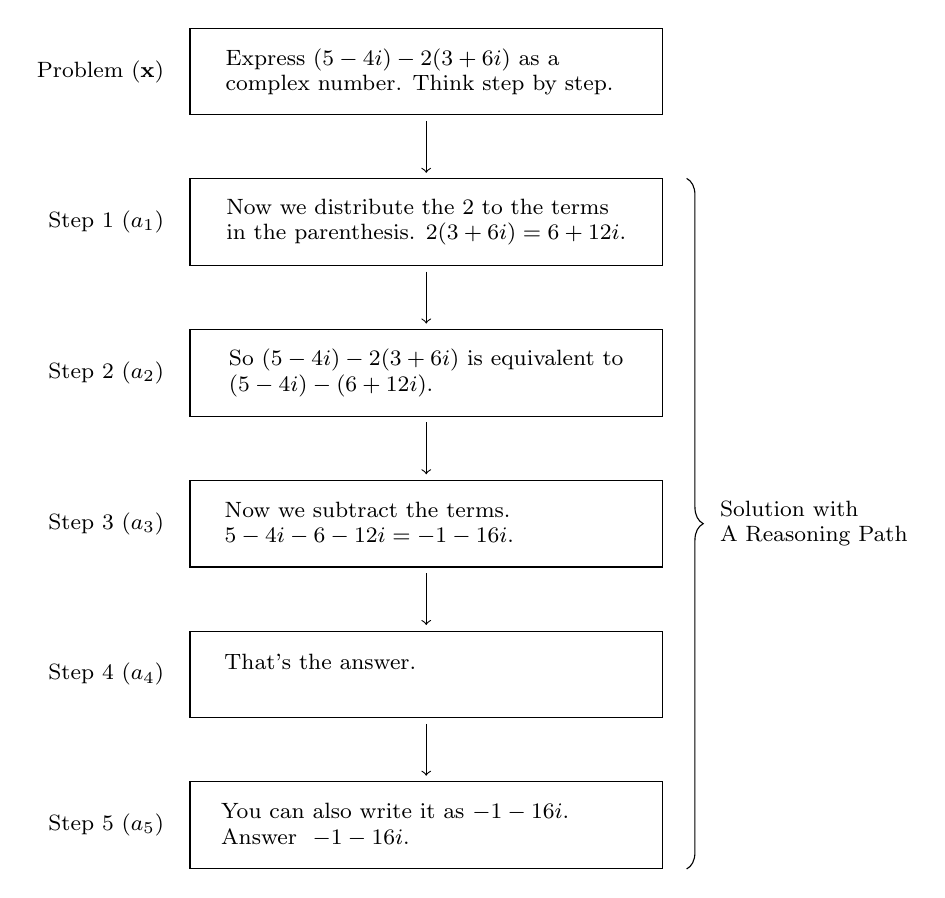
\begin{tikzpicture}
	
\def\ssep{0.1cm}
\def\bsep{2.5cm}

\tikzstyle{snode} = [minimum width=0.8cm,minimum height=0.5cm,inner sep=1pt,draw,thin];
\tikzstyle{rnode} = [minimum width=6cm,minimum height=1.1cm,inner sep=2pt,draw];

\begin{scope}

\node [rnode,anchor=west,align=left] (x) at (0,0) {\footnotesize{Express $(5-4i)-2(3+6i)$ as a \hspace{0.60cm}{\color{white} x}}\\[-0.1cm] \footnotesize{complex number. Think step by step.}};

\node [rnode,anchor=north west,align=left] (step1) at ([yshift=-0.8cm]x.south west) {\footnotesize{Now we distribute the $2$ to the terms}\\[-0.1cm] \footnotesize{in the parenthesis. $2(3+6i) = 6+12i$.}};

\node [rnode,anchor=north west,align=left] (step2) at ([yshift=-0.8cm]step1.south west) {\footnotesize{So $(5-4i)-2(3+6i)$ is equivalent to}\\[-0.1cm] \footnotesize{$(5-4i)-(6+12i)$.}};

\node [rnode,anchor=north west,align=left] (step3) at ([yshift=-0.8cm]step2.south west) {\footnotesize{Now we subtract the terms. \hspace{1.2cm}{\color{white} x}}\\[-0.1cm] \footnotesize{$5-4i-6-12i = -1-16i$.}};

\node [rnode,anchor=north west,align=left] (step4) at ([yshift=-0.8cm]step3.south west) {\footnotesize{That's the answer. \hspace{2.4cm}{\color{white} x}}\\[-0.1cm] \footnotesize{}};

\node [rnode,anchor=north west,align=left] (step5) at ([yshift=-0.8cm]step4.south west) {\footnotesize{You can also write it as $-1-16i$. \hspace{0.5cm}{\color{white} x}}\\[-0.1cm] \footnotesize{Answer\ \ $-1-16i$.}};

\draw [->] ([yshift=-2pt]x.south) -- ([yshift=2pt]step1.north);
\draw [->] ([yshift=-2pt]step1.south) -- ([yshift=2pt]step2.north);
\draw [->] ([yshift=-2pt]step2.south) -- ([yshift=2pt]step3.north);
\draw [->] ([yshift=-2pt]step3.south) -- ([yshift=2pt]step4.north);
\draw [->] ([yshift=-2pt]step4.south) -- ([yshift=2pt]step5.north);

\node [anchor=east] (xlabel) at ([xshift=-0.2cm]x.west) {\footnotesize{Problem ($\mathbf{x}$)}};
\node [anchor=east] (step1label) at ([xshift=-0.2cm]step1.west) {\footnotesize{Step 1 ($a_1$)}};
\node [anchor=east] (step2label) at ([xshift=-0.2cm]step2.west) {\footnotesize{Step 2 ($a_2$)}};
\node [anchor=east] (step3label) at ([xshift=-0.2cm]step3.west) {\footnotesize{Step 3 ($a_3$)}};
\node [anchor=east] (step4label) at ([xshift=-0.2cm]step4.west) {\footnotesize{Step 4 ($a_4$)}};
\node [anchor=east] (step5label) at ([xshift=-0.2cm]step5.west) {\footnotesize{Step 5 ($a_5$)}};

\draw [decoration={brace,amplitude=6pt},decorate] ([yshift=0.0cm,xshift=0.3cm]step1.north east) -- ([yshift=0.0cm,xshift=0.3cm]step5.south east) node [right,pos=0.5,xshift=0.3cm,align=left] {\footnotesize{Solution with}\\[-0.1cm] \footnotesize{A Reasoning Path}};


\end{scope}

\end{tikzpicture}
\end{center}

\vspace{-0.5cm} \caption{Illustration of multi-step reasoning. This example is from the PRM800K dataset~\cite{lightman-etal:2024lets}. Given a math problem, the LLM is prompted to generate a thinking path (or reasoning path) consisting of several reasoning steps. Each step addresses a sub-problem based on the results of the previous steps. The answer to the original problem is contained in the last step.}
\label{fig:multi-step-reasoning-example}
\end{figure}

The search algorithm can generate a set of candidate solutions:
\begin{eqnarray}
\mathcal{D}_c & = & \{\mathbf{y}_1,\cdots,\mathbf{y}_K\}.
\end{eqnarray}

Then, we can use a verifier, which evaluates each solution using the function $V(\mathbf{y})$, to score the candidates in $\mathcal{D}_c$. The final output is the best candidate selected by the verifier:
\begin{eqnarray}
\hat{\mathbf{y}} & = & \argmax_{\mathbf{y} \in \mathcal{D}_c} V(\mathbf{y}).
\end{eqnarray}

Although verifying the entire reasoning path is possible, a simpler alternative is to verify only the final reasoning step. In this way the verifier function $V(\mathbf{y})$ is simplified to depend solely on the final answer contained within $a_{n_r}$. This can be achieved in various ways, depending on the nature of the problem and the expected answer format.

\begin{itemize}
\item \vspace{0.5em} For some math and coding problems, we can use off-the-shelf tools as verifiers. Examples include proof checkers for mathematical theorems, interpreters or compilers for code execution, and unit test systems for verifying program correctness against predefined test cases.
\item \vspace{0.3em} If there is labeled data for evaluating the answer, such as human preference data, we can train a reward model on such data. The learned reward model is then used as the verifier which assigns a scalar score to each candidate answer.
\item \vspace{0.3em} If there are no existing systems or suitable reward models, we can use another LLM to act as the verifier. This LLM is prompted to assess the quality of the candidate answer. It could potentially be a more capable model, or the same LLM used with a specific ``evaluator'' prompt.
\item \vspace{0.3em} Alternatively, simpler heuristic-based verifiers can be designed. A commonly used approach is to employ majority voting, where the most frequently occurring answer among a set of candidates is selected.
\end{itemize}
\vspace{0.3em}

Using these verifiers, we can evaluate a set of candidate solutions generated during search. One simple strategy, which is often referred to as \mindex{parallel scaling}~\cite{brown-etal:2024large,snell-etal:2024scaling}, involves generating $K$ candidate solutions by running the base LLM $K$ times independently.  In this process, we can adjust the temperature in sampling to control the diversity in the outputs. The verifier then assesses each of these $K$ complete solutions, and the one with the highest score is selected as the final output. This is conceptually very similar to best-of-$N$ sampling, which in previous chapters we primarily described as a method of selecting the best one from a set of sampled outputs using a reward model.

Another approach is \mindex{sequential scaling}, which builds a sequence of solutions incrementally~\cite{gou-etal:2024critic,zhang-etal:2024small}. It starts with an initial solution generated by the LLM with prompting. Then, we use a verifier (often the same LLM) to evaluate the solution. This can be seen as a critique stage. The output of this stage is some form of feedback, such as textual critiques pinpointing errors or suggesting improvements, numerical scores reflecting solution quality, or even a revised plan or intermediate step to guide the next generation. This feedback, along with the original problem and the current solution, is then used to prompt the LLM to generate a potentially improved solution. This can be seen as a refine stage. This critique-refine cycle can be repeated, forming an iterative loop:
\begin{eqnarray}
\mathbf{y}_{k+1} & = & \mathrm{Refine}(\mathbf{x}, \mathbf{y}_k, \mathrm{Feedback}(\mathbf{y}_k)),
\end{eqnarray}

\noindent where $\mathrm{Feedback}(\mathbf{y}_k)$ represents the feedback from the verifier. The $\mathrm{Refine}(\cdot)$ function generates the improved solution $\mathbf{y}_{k+1}$ by prompting the LLM with the original problem $\mathbf{x}$, the previous solution $\mathbf{y}_k$, and this feedback. The process can be repeated for $K$ iterations, or until the solution quality, as assessed by the verifier, converges to a satisfactory level. This iterative framework, where a solution is progressively improved through cycles of generation, evaluation (critique), and revision, is precisely what constitutes self-refinement~\cite{shinn-etal:2023reflexion,madaan-etal:2024self}. In such scenarios, the role of the verifier is not just to pick the best complete solution from a static set, but to actively guide the generation process itself.

See Figure~\ref{fig:parallel-and-sequential-scaling} for illustrations of parallel scaling and sequential scaling. Note that there are other ways to perform search and obtain different sets of candidate solutions. One alternative method is to organize the search as a tree structure. This approach, often referred to as tree search, provides a more structured way to explore the space of possible reasoning paths. In solution-level search, each node of the tree represents a complete solution. During search, we need to expand a node into a set of child nodes, representing new solutions that can be considered in verification. The expansion process typically involves taking an existing solution (the parent node) and using the LLM to generate variations or alternative solutions.

\begin{figure}[!t]
\centering
% !Mode:: "TeX:UTF-8"
% !TEX encoding = UTF-8 Unicode

\begin{center}
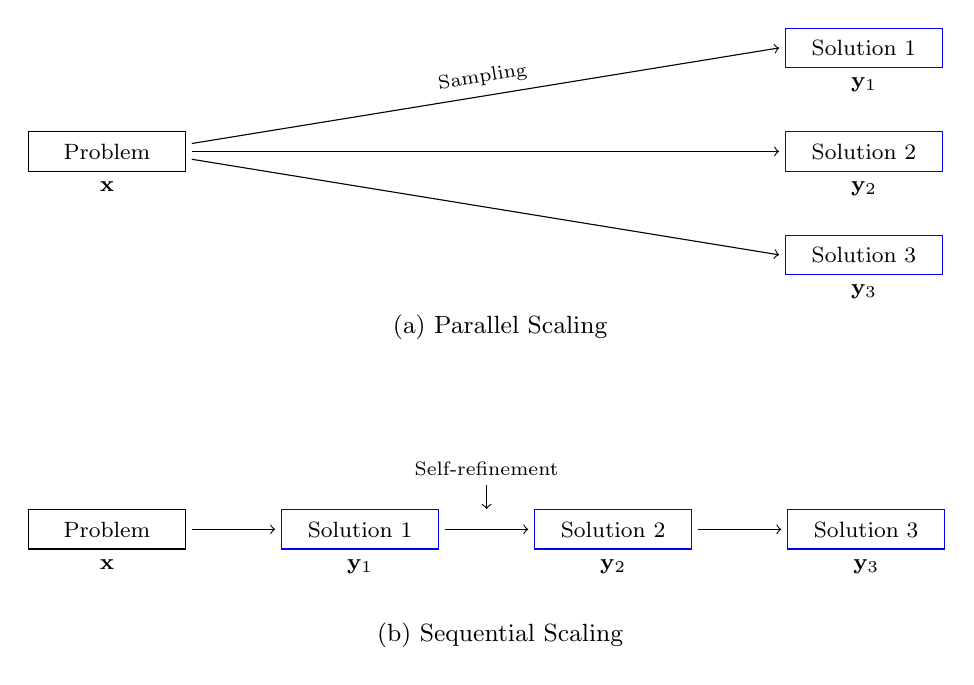
\begin{tikzpicture}
	
\def\ssep{0.1cm}
\def\bsep{2.5cm}

\tikzstyle{snode} = [minimum width=0.8cm,minimum height=0.5cm,inner sep=1pt,draw,thin];
\tikzstyle{rnode} = [minimum width=2cm,minimum height=0.5cm,inner sep=2pt,draw];

% parallel scaling
\begin{scope}

\node [rnode,anchor=west] (x) at (0,0) {\footnotesize{Problem}};

\node [rnode,anchor=west,draw=blue] (s2) at ([xshift=7.6cm]x.east) {\footnotesize{Solution 2}};
\node [rnode,anchor=south west,draw=blue] (s1) at ([yshift=0.8cm]s2.north west) {\footnotesize{Solution 1}};
\node [rnode,anchor=north west,draw=blue] (s3) at ([yshift=-0.8cm]s2.south west) {\footnotesize{Solution 3}};

\node [anchor=north] (xlabel) at (x.south) {\footnotesize{$\mathbf{x}$}};
\node [anchor=north] (s1label) at (s1.south) {\footnotesize{$\mathbf{y}_1$}};
\node [anchor=north] (s2label) at (s2.south) {\footnotesize{$\mathbf{y}_2$}};
\node [anchor=north] (s3label) at (s3.south) {\footnotesize{$\mathbf{y}_3$}};

\draw [->] ([xshift=2pt,yshift=0.1cm]x.east) -- ([xshift=-2pt]s1.west) node [pos=0.5,above,rotate=9] {\scriptsize{Sampling}};
\draw [->] ([xshift=2pt,yshift=0.0cm]x.east) -- ([xshift=-2pt]s2.west);
\draw [->] ([xshift=2pt,yshift=-0.1cm]x.east) -- ([xshift=-2pt]s3.west);

\node [anchor=north west] (caption) at ([yshift=-1.7cm,xshift=2.5cm]x.south east) {\small{(a) Parallel Scaling}};

\end{scope}

% sequential scaling
\begin{scope}[yshift=-4.8cm]

\node [rnode,anchor=west] (x) at (0,0) {\footnotesize{Problem}};

\node [rnode,anchor=west,draw=blue] (s1) at ([xshift=1.2cm]x.east) {\footnotesize{Solution 1}};
\node [rnode,anchor=west,draw=blue] (s2) at ([xshift=1.2cm]s1.east) {\footnotesize{Solution 2}};
\node [rnode,anchor=west,draw=blue] (s3) at ([xshift=1.2cm]s2.east) {\footnotesize{Solution 3}};

\node [anchor=north] (xlabel) at (x.south) {\footnotesize{$\mathbf{x}$}};
\node [anchor=north] (s1label) at (s1.south) {\footnotesize{$\mathbf{y}_1$}};
\node [anchor=north] (s2label) at (s2.south) {\footnotesize{$\mathbf{y}_2$}};
\node [anchor=north] (s3label) at (s3.south) {\footnotesize{$\mathbf{y}_3$}};

\draw [->] ([xshift=2pt]x.east) -- ([xshift=-2pt]s1.west);
\draw [->] ([xshift=2pt]s1.east) -- ([xshift=-2pt]s2.west);
\draw [->] ([xshift=2pt]s2.east) -- ([xshift=-2pt]s3.west);

\node [anchor=south] (selflabel) at ([xshift=0.6cm,yshift=0.3cm]s1.north east) {\scriptsize{Self-refinement}};
\draw [->,thin] (selflabel.south) -- ([yshift=-0.3cm]selflabel.south);

\node [anchor=north west] (caption) at ([yshift=-0.8cm,xshift=2.3cm]x.south east) {\small{(b) Sequential Scaling}};

\end{scope}

\end{tikzpicture}
\end{center}

\vspace{-0.5cm} \caption{Illustrations of parallel scaling and sequential scaling. In parallel scaling, we obtain multiple solutions by running the LLM several times independently. In sequential scaling, the LLM generates an initial solution. Then, we use the LLM to refine it iteratively, with each refinement yielding a new, possibly better solution.}
\label{fig:parallel-and-sequential-scaling}
\end{figure}

\subsubsection{Step-level Search with Verifiers}

While the methods discussed above primarily focus on generating complete solutions before final selection, the search process can also be integrated more deeply into the step-by-step generation of the reasoning path itself. This leads to approaches that perform step-level search with verifiers, where guidance or pruning occurs at intermediate reasoning steps $\{a_1,\cdots,a_{i}\}$ rather than only after a full solution $\mathbf{y}$ is formed.

Such fine-grained control is particularly beneficial for complex reasoning problems where a single incorrect intermediate step can render the entire subsequent reasoning chain invalid. By evaluating or guiding the generation at each intermediate step, the LLM can explore the reasoning space more effectively, potentially pruning unpromising paths early or allocating more resources to explore more plausible ones.

Step-level search with verifiers can also be modeled as a tree search problem. In this paradigm, each node (or state) corresponds to a partial reasoning path, $\mathbf{a}_{\le i} = (a_1,\cdots,a_i)$, representing the sequence of $i$ reasoning steps taken so far (i.e., a path from the root node to the current node). The objective of the search process is to explore the underlying state space, starting from an initial empty path, to find a complete path that constitutes a correct solution. Note that we use $\mathbf{a}_{\le i}$ here to represent a partial reasoning path instead of $\mathbf{y}_{\le i}$. While this makes notation a bit inconsistent with that used for representing complete solutions ($\mathbf{y}$) or full paths in solution-level search, it serves to highlight the focus on individual actions or steps.

The core components of step-level search with verifiers are:

\begin{itemize}
\item \vspace{0.5em} \textbf{Node Representation}. A node is a partial reasoning path $\mathbf{a}_{\le i} = (a_1,\cdots,a_i)$. The root node is an empty path, and terminal nodes are complete reasoning paths.
\item \vspace{0.3em} \textbf{Node Expansion}. Given a current partial path $\mathbf{a}_{\le i}$, the LLM is used to generate one or more candidate next reasoning steps $\{a_{i+1}^{(1)},\cdots,a_{i+1}^{(M)}\}$. Each candidate step, when appended to $\mathbf{a}_{\le i}$, forms a new potential partial path $\mathbf{a}_{\le i + 1} = (a_1,\cdots,a_i,a_{i+1}^{(j)})$.
\item \vspace{0.3em} \textbf{Verification}. The verifier $V(\cdot)$ evaluates the quality of a newly generated step in the context of the current partial path $\mathbf{a}_{\le i} = (a_1,\cdots,a_i)$ and the original problem $\mathbf{x}$. As with solution-level verification, step-level verifiers might output a numerical score, a categorical label, or textual feedback.
\item \vspace{0.3em} \textbf{Search}. This governs how the search space is explored. Based on the evaluations from the verifier, the search strategy decides which partial paths to extend further, which to prune, and the order of exploration.
\end{itemize}
\vspace{0.5em}

This step-by-step verification allows for dynamic adjustments to the reasoning process. If a step $a_{i+1}$ is deemed incorrect or unpromising by $V(\cdot)$, the search algorithm can backtrack and explore alternative steps from $\mathbf{a}_{\le i}$, or even from an earlier node $\mathbf{a}_{\le i'}$ (where $i' < i$). Conversely, if a step is highly rated, resources can be focused on extending that path. See Figure~\ref{fig:step-level-search-with-verifiers} for an illustration of step-level search with verifiers.

\begin{figure}[!t]
\centering
% !Mode:: "TeX:UTF-8"
% !TEX encoding = UTF-8 Unicode

\begin{center}
\begin{tikzpicture}
	
\def\ssep{1cm}
\def\vsep{1.5cm}

\tikzstyle{snode} = [minimum width=0.28cm,minimum height=0.28cm,inner sep=0pt];
\tikzstyle{rnode} = [minimum width=1.2cm,minimum height=0.7cm,inner sep=2pt,draw];

% step-level verification
\begin{scope}

\node [rnode,anchor=west,thick,red] (root) at (0,0) {\footnotesize{$\mathbf{x}$}};

\node [rnode,anchor=north] (s13) at ([yshift=-\vsep]root.south) {{\footnotesize{$a_{1}^{(3)}$}}};
\node [rnode,anchor=east] (s12) at ([xshift=-0.5*\ssep]s13.west) {{\footnotesize{$a_{1}^{(2)}$}}};
\node [rnode,anchor=east] (s11) at ([xshift=-0.5*\ssep]s12.west) {{\footnotesize{$a_{1}^{(1)}$}}};
\node [rnode,anchor=west,thick,red] (s14) at ([xshift=0.5*\ssep]s13.east) {{\footnotesize{$a_{1}^{(4)}$}}};
\node [rnode,anchor=west] (s15) at ([xshift=0.5*\ssep]s14.east) {{\footnotesize{$a_{1}^{(5)}$}}};

\node [snode,anchor=center,fill=white] (l11) at ([xshift=-1pt,yshift=1pt]s11.south east) {\color{blue} \small{$\boxtimes$}};
\node [snode,anchor=center,fill=white] (l12) at ([xshift=-1pt,yshift=1pt]s12.south east) {\color{ugreen} \small{$\boxtimes$}};
\node [snode,anchor=center,fill=white] (l13) at ([xshift=-1pt,yshift=1pt]s13.south east) {\color{ugreen} \small{$\boxtimes$}};
\node [snode,anchor=center,fill=white] (l15) at ([xshift=-1pt,yshift=1pt]s15.south east) {\color{blue} \small{$\boxtimes$}};

\draw [-latex] ([xshift=-0.2cm,yshift=-2pt]root.south) -- ([xshift=0.4cm,yshift=2pt]s11.north);
\draw [-latex] ([xshift=-0.1cm,yshift=-2pt]root.south) -- ([xshift=0.2cm,yshift=2pt]s12.north);
\draw [-latex] ([xshift=0.0cm,yshift=-2pt]root.south) -- ([xshift=0.0cm,yshift=2pt]s13.north);
\draw [-latex,thick,red] ([xshift=0.1cm,yshift=-2pt]root.south) -- ([xshift=-0.2cm,yshift=2pt]s14.north);
\draw [-latex] ([xshift=0.2cm,yshift=-2pt]root.south) -- ([xshift=-0.4cm,yshift=2pt]s15.north);

\node [rnode,anchor=north,thick,red] (s23) at ([yshift=-\vsep]s14.south) {{\footnotesize{$a_{2}^{(3)}$}}};
\node [rnode,anchor=east] (s22) at ([xshift=-0.5*\ssep]s23.west) {{\footnotesize{$a_{2}^{(2)}$}}};
\node [rnode,anchor=east] (s21) at ([xshift=-0.5*\ssep]s22.west) {{\footnotesize{$a_{2}^{(1)}$}}};
\node [rnode,anchor=west] (s24) at ([xshift=0.5*\ssep]s23.east) {{\footnotesize{$a_{2}^{(4)}$}}};
\node [rnode,anchor=west] (s25) at ([xshift=0.5*\ssep]s24.east) {{\footnotesize{$a_{2}^{(5)}$}}};

\node [snode,anchor=center,fill=white] (l21) at ([xshift=-1pt,yshift=1pt]s21.south east) {\color{ugreen} \small{$\boxtimes$}};
\node [snode,anchor=center,fill=white] (l22) at ([xshift=-1pt,yshift=1pt]s22.south east) {\color{blue} \small{$\boxtimes$}};
\node [snode,anchor=center,fill=white] (l24) at ([xshift=-1pt,yshift=1pt]s24.south east) {\color{ugreen} \small{$\boxtimes$}};
\node [snode,anchor=center,fill=white] (l25) at ([xshift=-1pt,yshift=1pt]s25.south east) {\color{ugreen} \small{$\boxtimes$}};

\draw [-latex] ([xshift=-0.2cm,yshift=-2pt]s14.south) -- ([xshift=0.4cm,yshift=2pt]s21.north);
\draw [-latex] ([xshift=-0.1cm,yshift=-2pt]s14.south) -- ([xshift=0.2cm,yshift=2pt]s22.north);
\draw [-latex,thick,red] ([xshift=0.0cm,yshift=-2pt]s14.south) -- ([xshift=0.0cm,yshift=2pt]s23.north);
\draw [-latex] ([xshift=0.1cm,yshift=-2pt]s14.south) -- ([xshift=-0.2cm,yshift=2pt]s24.north);
\draw [-latex] ([xshift=0.2cm,yshift=-2pt]s14.south) -- ([xshift=-0.4cm,yshift=2pt]s25.north);

\node [rnode,anchor=north] (s33) at ([yshift=-\vsep]s23.south) {{\footnotesize{$a_{3}^{(3)}$}}};
\node [rnode,anchor=east] (s32) at ([xshift=-0.5*\ssep]s33.west) {{\footnotesize{$a_{3}^{(2)}$}}};
\node [rnode,anchor=east,thick,red] (s31) at ([xshift=-0.5*\ssep]s32.west) {{\footnotesize{$a_{3}^{(1)}$}}};
\node [rnode,anchor=west] (s34) at ([xshift=0.5*\ssep]s33.east) {{\footnotesize{$a_{3}^{(4)}$}}};
\node [rnode,anchor=west] (s35) at ([xshift=0.5*\ssep]s34.east) {{\footnotesize{$a_{3}^{(5)}$}}};

\node [snode,anchor=center,fill=white] (l32) at ([xshift=-1pt,yshift=1pt]s32.south east) {\color{ugreen} \small{$\boxtimes$}};
\node [snode,anchor=center,fill=white] (l33) at ([xshift=-1pt,yshift=1pt]s33.south east) {\color{blue} \small{$\boxtimes$}};
\node [snode,anchor=center,fill=white] (l34) at ([xshift=-1pt,yshift=1pt]s34.south east) {\color{ugreen} \small{$\boxtimes$}};
\node [snode,anchor=center,fill=white] (l35) at ([xshift=-1pt,yshift=1pt]s35.south east) {\color{blue} \small{$\boxtimes$}};

\draw [-latex,thick,red] ([xshift=-0.2cm,yshift=-2pt]s23.south) -- ([xshift=0.4cm,yshift=2pt]s31.north);
\draw [-latex] ([xshift=-0.1cm,yshift=-2pt]s23.south) -- ([xshift=0.2cm,yshift=2pt]s32.north);
\draw [-latex] ([xshift=0.0cm,yshift=-2pt]s23.south) -- ([xshift=0.0cm,yshift=2pt]s33.north);
\draw [-latex] ([xshift=0.1cm,yshift=-2pt]s23.south) -- ([xshift=-0.2cm,yshift=2pt]s34.north);
\draw [-latex] ([xshift=0.2cm,yshift=-2pt]s23.south) -- ([xshift=-0.4cm,yshift=2pt]s35.north);

\node [rnode,anchor=north,thick,red] (s43) at ([yshift=-\vsep]s31.south) {{\footnotesize{$a_{4}^{(3)}$}}};
\node [rnode,anchor=east] (s42) at ([xshift=-0.5*\ssep]s43.west) {{\footnotesize{$a_{4}^{(2)}$}}};
\node [rnode,anchor=east] (s41) at ([xshift=-0.5*\ssep]s42.west) {{\footnotesize{$a_{4}^{(1)}$}}};
\node [rnode,anchor=west] (s44) at ([xshift=0.5*\ssep]s43.east) {{\footnotesize{$a_{4}^{(4)}$}}};
\node [rnode,anchor=west] (s45) at ([xshift=0.5*\ssep]s44.east) {{\footnotesize{$a_{4}^{(5)}$}}};

\node [snode,anchor=center,fill=white] (l41) at ([xshift=-1pt,yshift=1pt]s41.south east) {\color{ugreen} \small{$\boxtimes$}};
\node [snode,anchor=center,fill=white] (l42) at ([xshift=-1pt,yshift=1pt]s42.south east) {\color{blue} \small{$\boxtimes$}};
\node [snode,anchor=center,fill=white] (l44) at ([xshift=-1pt,yshift=1pt]s44.south east) {\color{blue} \small{$\boxtimes$}};
\node [snode,anchor=center,fill=white] (l45) at ([xshift=-1pt,yshift=1pt]s45.south east) {\color{blue} \small{$\boxtimes$}};

\draw [-latex] ([xshift=-0.2cm,yshift=-2pt]s31.south) -- ([xshift=0.4cm,yshift=2pt]s41.north);
\draw [-latex] ([xshift=-0.1cm,yshift=-2pt]s31.south) -- ([xshift=0.2cm,yshift=2pt]s42.north);
\draw [-latex,thick,red] ([xshift=0.0cm,yshift=-2pt]s31.south) -- ([xshift=0.0cm,yshift=2pt]s43.north);
\draw [-latex] ([xshift=0.1cm,yshift=-2pt]s31.south) -- ([xshift=-0.2cm,yshift=2pt]s44.north);
\draw [-latex] ([xshift=0.2cm,yshift=-2pt]s31.south) -- ([xshift=-0.4cm,yshift=2pt]s45.north);

\begin{pgfonlayer}{background}
\node [draw,dashed,inner sep=2pt]  [fit = (root)] (rootbox) {};
\node [anchor=south west] (xlabel) at ([yshift=0.2cm,xshift=0.3cm]rootbox.north east) {\scriptsize{Input Problem (Root)}};
\draw [->] ([xshift=0.2cm,yshift=0.1cm]xlabel.south west) -- ([yshift=-0.1cm,xshift=2pt]rootbox.north east);

\node [draw,dashed,inner sep=2pt]  [fit = (s11) (l11)] (s11box) {};
\node [anchor=south] (s11label) at ([yshift=0.2cm,xshift=-1cm]s11box.north) {\scriptsize{Pruned by Likelihood}};
\draw [->] ([xshift=0.5cm,yshift=0.1cm]s11label.south) -- ([yshift=2pt,xshift=-0.3cm]s11box.north);

\node [draw,dashed,inner sep=2pt]  [fit = (s21) (l21)] (s21box) {};
\node [anchor=south] (s21label) at ([yshift=0.2cm,xshift=-1cm]s21box.north) {\scriptsize{Pruned by Verification}};
\draw [->] ([xshift=0.5cm,yshift=0.1cm]s21label.south) -- ([yshift=2pt,xshift=-0.3cm]s21box.north);

\node [draw,dashed,inner sep=2pt]  [fit = (s31)] (s31box) {};
\node [anchor=south] (s31label) at ([yshift=0.2cm,xshift=-1cm]s31box.north) {\scriptsize{Selected Reasoning Step}};
\draw [->] ([xshift=0.5cm,yshift=0.1cm]s31label.south) -- ([yshift=2pt,xshift=-0.3cm]s31box.north);

\end{pgfonlayer}

\end{scope}

\end{tikzpicture}
\end{center}

\vspace{-0.5cm} \caption{Illustration of step-level search with verifiers. $a_{i}^{(j)}$ = the $j$-th candidate for the $i$-th reasoning step, {\color{blue} $\boxtimes$} = candidate pruned by the LLM's output probability, and {\color{ugreen} $\boxtimes$} = candidate pruned by the verifier. Given the input problem as the root node, we expand the tree by generating multiple reasoning steps at each expansion. Each candidate can be pruned by either likelihood (as in standard decoding) or step-level verification. The unpruned candidates are then expanded to generate further reasoning steps. The process is iterated until a complete reasoning chain leading to a final answer is generated, or until a predefined search limit is reached.}
\label{fig:step-level-search-with-verifiers}
\end{figure}

Clearly, this search framework is very similar to that used in decoding methods for LLMs, as discussed in Section~\ref{sec:llm-decoding-algorithms}. For example, beam search maintains a set of $K$ most promising partial sequences at each generation step. This is a form of step-level search where the ``verifier'' is implicitly the LLM's own probability model, and the ``search'' is the pruning mechanism to maintain the beam size.

However, step-level search with explicit verifiers, as described here, is different from standard decoding methods. One key difference is that the verifier can be a much more sophisticated component than just the raw output probabilities of the generative LLM. The design of step-level verifiers follows a design similar to solution-level verification. A step-level verifier might be a language model that assesses the quality of an individual reasoning step within the context of the preceding path. This LLM can even be fine-tuned to enhance its verification capability. Alternatively, for domains with well-defined rules, it could be a symbolic engine or a set of programmatic checks. Furthermore, verifiers can be designed to predict the future utility or likelihood of success given the current partial path, drawing inspiration from value functions in reinforcement learning. Human expertise can also be incorporated to provide judgments on critical steps, especially in high-stakes scenarios.

One example of such a step-level verifier, particularly when using human feedback to assess intermediate progress, is the \mindex{process reward model} (\mindex{PRM}).  A PRM is typically a separate language model trained to output a scalar reward for each reasoning step $a_{i'}$ within a partial path $\mathbf{a}_{\le i}$. It provides a more direct and fine-grained supervisory signal compared to \mindex{outcome reward models} (\mindex{ORMs}) which only evaluate the final solution. However, the development of PRMs relies on step-level human annotations, such as preferences on different next steps. Collecting supervision for each intermediate step is considerably more labor-intensive and requires greater cognitive effort from human annotators than simply labeling final outcomes.

One alternative approach to developing training data for step-level verification is to use LLMs to generate such annotations automatically. For example, we can take a strong LLM, referred to as a teacher model, and prompt it to first generate a complete reasoning path for a given problem. Then, at each intermediate step within this path, we can prompt the same teacher LLM (or another capable LLM) to generate several alternative candidate next steps in addition to the one it originally chose. The teacher LLM can then be prompted again to evaluate these alternatives. These evaluation results (e.g., correct vs. incorrect) can then serve as data annotations. Alternatively, the generalization capabilities of PRMs can be leveraged. We can train a PRM on tasks where step-level verification is easier and then generalize this PRM to other tasks with little or no additional training.

Note that step-level verification also comes with its own problems. Frequent verification, especially if using an LLM as the verifier, can substantially increase computational costs and latency. The design of effective step-level verifiers is non-trivial itself. An inaccurate verifier might prematurely discard good reasoning paths or fail to identify flawed ones, thereby misleading the search. This makes the development of such systems more difficult.

\subsubsection{Encouraging Long Thinking}

So far in this subsection, most of the methods are implicitly based on a simple idea: generating longer reasoning paths can help. In addition to CoT and search with verification, we can consider alternative methods to achieve this. For example, we can prompt the LLM by explicitly asking for extended deliberation. Beyond direct prompting, we can also make modifications to the decoding process itself, such as adjusting token limits or applying penalties for short outputs. Another approach is to employ multi-stage generation schemes where the model incrementally builds upon its reasoning.

\subsubsection{Training-based Scaling}

As well as considering inference-time scaling methods without training, we also wish to consider methods that can improve intrinsic reasoning capabilities of LLMs by modifying their parameters through further training. While such training-based scaling methods typically require additional training cost and computational resources, they embed stronger reasoning skills directly into the model parameters, which in turn can lead to improved reasoning performance. We can even combine them with training-free methods to further improve inference-time scaling.

Although our discussion here is restricted to reasoning problems, methods for training-based scaling are common. Most of them have been discussed in Chapter \ChapterLLMTuning. Here, we will briefly describe how these methods can be applied to improving inference-time scaling for reasoning problems.

\begin{itemize}
\item \vspace{0.5em} \textbf{Fine-tuning on Reasoning Data}. One of the most direct ways to enhance reasoning is by fine-tuning pre-trained LLMs on datasets specifically curated for reasoning tasks. These datasets can range from simple input-output pairs to more structured formats that include step-by-step reasoning processes. Typical examples include datasets of math word problems, logical deduction exercises, or code generation with explanations. By training on such data, the model learns from common reasoning patterns, and thus can generate detailed and coherent reasoning paths at test time.
\item \vspace{0.3em} \textbf{Reinforcement Learning for Reasoning}. If we regard a verifier as a reward model, we can see that the methods discussed in the previous subsection are a direct application of the reward model to reasoning problems, though they are training-free. Of course, we can apply this reward model to LLM fine-tuning. This follows a standard paradigm of reinforcement learning. Given a reward model, the LLM, acting as a policy, is fine-tuned using reinforcement learning algorithms. The LLM generates reasoning steps or full solutions, receives feedback (rewards) from the reward model, and updates its parameters to produce outputs that maximize these rewards. This process aligns the LLM outputs with high-quality reasoning behavior, thereby encouraging the LLM to generate more reliable reasoning paths. Another key problem is the training of the reward model. Generally, this reward model could be an outcome reward model that evaluates the correctness or quality of the final answer, or a process reward model that assesses the quality of each intermediate reasoning step, as discussed in the context of step-level verifiers. In some cases, we can even develop a reward model based on simple rules, such as giving bonuses to longer outputs.
\item \vspace{0.3em} \textbf{Knowledge Distillation for Reasoning}. In this approach, a smaller, more efficient student LLM is trained to mimic the reasoning outputs or internal representations of a larger, more capable teacher LLM. The teacher model might generate detailed reasoning steps for a variety of problems. The student model then learns to reproduce these high-quality reasoning demonstrations. This strategy makes stronger reasoning capabilities more accessible by deploying them in smaller models that are less computationally expensive at inference time.
\item \vspace{0.3em} \textbf{Iterative Refinement}. Training-based scaling can also involve iterative refinement. For example, an LLM can generate solutions to a set of problems. These solutions and their reasoning paths are then verified, either by humans or automatic verifiers. The correct reasoning paths are subsequently added to the training data, and the LLM is further fine-tuned on this augmented dataset. This creates a cycle where the LLM progressively improves its reasoning capabilities through repeated generation, critique, and learning.
\end{itemize}
\vspace{0.5em}

The primary advantage of these training-based scaling methods is that they endow the LLM with stronger inherent reasoning skills. This directly contributes to improved inference-time scaling in several ways: it can lead to more efficient inference, as the LLM might require less extensive search or fewer generation samples to arrive at a correct solution. Moreover, the base quality of generated steps or solutions is higher. Therefore, a well-trained LLM might generalize its learned reasoning abilities to novel problems more effectively than an LLM relying solely on in-context learning or training-free inference schemes.

On the other hand, training-based approaches also present challenges, compared to the training-free counterparts. The creation of high-quality, large-scale training datasets for reasoning can be expensive and labor-intensive. The fine-tuning process itself, particularly for the largest LLMs or when using RL, can be computationally intensive and require substantial engineering effort. There is also the risk of the model overfitting to the specific types of problems or reasoning styles present in the training data, potentially limiting its performance on out-of-distribution tasks.

%----------------------------------------------------------------------------------------
% NEW SECTION
%----------------------------------------------------------------------------------------

\section{Summary}

In this chapter, we have discussed inference for LLMs. We have presented the prefilling-decoding framework and related decoding algorithms for LLM inference. Then, we have described several techniques for efficient inference. We have also discussed inference-time scaling, which is one of the most important approaches to improving LLM reasoning.

Inference over sequential data has long been a fundamental topic in AI~\cite{wozengraft-and-reiffen:1961,viterbi:1967error,forney-etal:1972maximum}. In the context of NLP, this line of work dates back to the very early days of speech recognition and statistical machine translation~\cite{Koehn:2010}, where researchers faced the challenge of efficiently searching vast hypothesis spaces to find the most probable output sequence. Techniques like beam search and various pruning strategies were developed then to make this computationally tractable. At that time, models were relatively weak, and much of the research focused on developing powerful search algorithms to reduce search errors. These foundational ideas continue to influence modern approaches.

As we enter the era dominated by deep learning methods, models based on deep neural networks have become extremely powerful. Even with very simple search algorithms, these models can achieve excellent results. In this context, inference no longer seems as ``important'' as it once was, and research attention has gradually shifted toward model architectures, training methods, and scaling up models.

However, this trend has recently shifted. With the rise of LLMs, inference has once again attracted significant attention. This renewed focus is primarily reflected in two aspects:

\begin{itemize}
\item \vspace{0.5em} The inference cost for LLMs is very high. For example, efficiently deploying LLMs in high-concurrency, low-latency scenarios remains a challenging problem, making inference efficiency critically important. In this context, efficient architecture designs, optimized search algorithms, and various inference optimization strategies hold substantial practical significance.
\item \vspace{0.3em} Input and output sequence lengths have significantly increased in complex tasks. Especially in tasks like mathematical reasoning, the growth of sequence lengths further highlights the importance of inference efficiency. Moreover, scaling the inference process has recently proven to be an effective way to improve the reasoning capabilities of models. Therefore, achieving efficient inference scaling is emerging as a particularly promising research direction.
\end{itemize}
\vspace{0.5em}

Inference is now a wide-ranging topic that encompasses many techniques. It involves not only the development of model architectures and decoding algorithms, but is increasingly shaped by the intricate engineering and sophisticated systems-level optimizations required to deploy LLMs effectively and efficiently. Many of these techniques are beyond the scope of NLP or a specific AI area. Instead, the frontier of LLM inference optimization now extends deeply into domains traditionally considered core computer science and engineering.

